\chapter{中枢神经系统的突触整合} \label{chap:chap13}

与神经肌肉接头处的突触传递一样,中枢神经系统神经元之间最快速的信号传递涉及突触后膜中的离子型受体。
因此,许多适用于神经肌肉接头处运动神经元和骨骼肌纤维之间突触连接的原理也适用于中枢神经系统。
然而,由于多种原因,中枢神经元之间的突触传递更为复杂。


首先,尽管大多数肌肉纤维通常仅受一个运动神经元支配,但一个中枢神经细胞(例如新皮层中的锥体神经元)\textit{接收}来自数千个神经元的连接。
其次,肌肉纤维只接收兴奋性输入,而中枢神经元同时接收兴奋性和\textit{抑制}性输入。
第三,肌肉纤维上的所有突触作用均由\textit{一种}神经递质乙酰胆碱介导,它仅激活一种类型的受体(离子型烟碱乙酰胆碱受体)。
然而,单个中枢神经元可以对许多不同类型的输入作出反应,每种输入都由激活特定类型受体的不同递质介导。 
这些受体包括离子型受体,其中递质的结合直接打开离子通道,以及代谢型受体,其中递质结合通过激活第二信使间接调节通道。
因此,与肌肉纤维不同,中枢神经元必须将不同的输入整合到一个单一的协调动作中。


最后,神经-肌肉突触是效率模型——运动神经元中的每个动作电位都会在肌纤维中产生一个动作电位。
相比之下,突触前神经元与中枢神经元之间的连接效果有限——在许多情况下,至少 50 到 100 个兴奋性神经元必须同时激发才能产生足够大的突触电位,以触发突触后神经元的动作电位。


对中枢神经系统突触传递的第一个见解来自\textit{约翰·埃克尔斯}和他的同事在 1950 年代的实验,该实验研究了突触输入到控制牵张反射的脊髓运动神经元,这是我们在第~\ref{chap:chap3}~章中考虑的简单行为。
脊髓运动神经元 对于检查中枢突触机制特别有用,因为它们具有大的、可接近的细胞体,最重要的是,它们同时接收兴奋性和抑制性连接,因此使我们能够在细胞水平上研究神经系统的综合作用。



\section{中枢神经元接收兴奋性和抑制性输入}

为了分析介导牵张反射的突触,\textit{埃克尔斯}激活了大量的感觉细胞轴突,这些轴突支配股四头肌(伸肌)中的牵张受体器官(图~\ref{fig:13_1}A、B)。 
如今,同样的实验可以通过刺激单个感觉神经元来完成。


\begin{figure}[htbp]
	\centering
	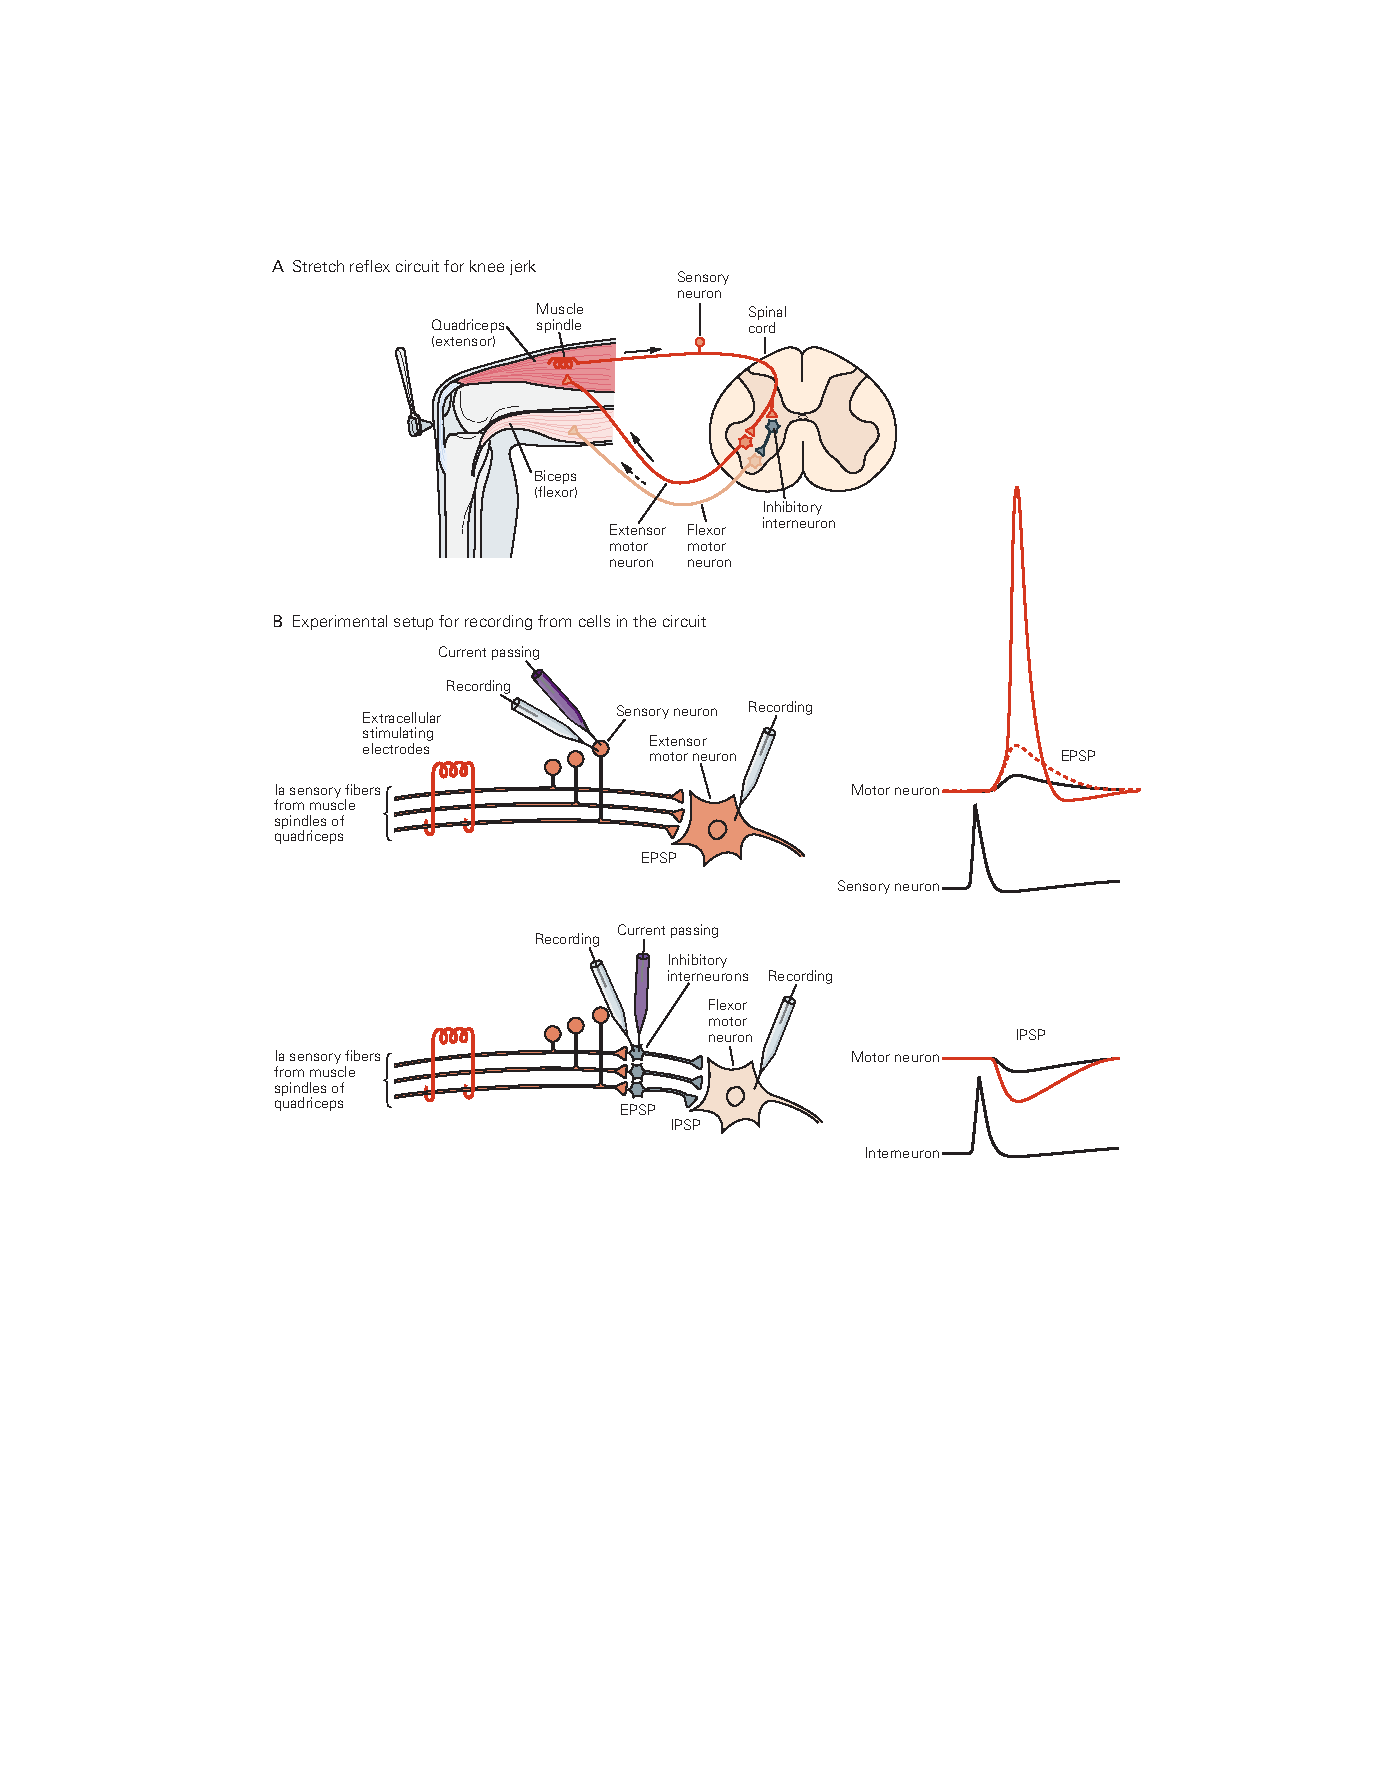
\includegraphics[width=0.85\linewidth]{chap13/fig_13_1}
	\caption{介导\textit{股四头肌}牵张反射的兴奋性和抑制性突触连接的组合是中枢神经系统回路的典型特征。
		\textbf{A.} 由伸肌(股四头肌)上的牵张感受器(肌梭)激活的感觉神经元与支配同一肌肉群的脊髓中的伸肌运动神经元产生兴奋性连接。
		它还与中间神经元建立兴奋性联系,后者又与支配拮抗肌(股二头肌)肌肉群的屈肌运动神经元建立抑制性联系。
		相反,来自二头肌的传入纤维(未显示)激发中间神经元,从而在伸肌运动神经元上形成抑制性突触。
		\textbf{B.} 这个理想化的实验装置展示了研究 A 部分所示通路中运动神经元的抑制和兴奋的方法。
		上图:在伸肌运动神经元中引发\textit{兴奋性突触后电位}的两种选择。
		可以通过将电流通过的电极插入感觉神经元细胞体来刺激单个突触前轴突。
		以这种方式刺激的感觉神经元中的动作电位会触发伸肌运动神经元中的小\textit{兴奋性突触后电位}(黑色轨迹)。
		或者,可以用细胞外电极电刺激股四头肌的整个传入神经。
		通过细胞外电极激发许多传入神经元会产生足够大的突触电位(虚线)以启动动作电位(红色迹线)。
		下图:用于引发和测量屈肌运动神经元抑制电位的设置。
		接受来自股四头肌通路输入的单个抑制性中间神经元的细胞内刺激在屈肌运动神经元(黑色迹线)中产生小的\textit{抑制性突触后电位}(超极化)。
		细胞外刺激募集大量抑制性神经元并产生更大的 IPSP(红色迹线)。 (感觉神经元和中间神经元的动作电位显得较小,因为它们的放大率低于运动神经元。)}
	\label{fig:13_1}
\end{figure}


通过微电极将足够的电流传递到支配伸肌的牵张感受器感觉神经元的细胞体中会产生动作电位。
这反过来会在运动神经元中产生一个小的\textit{兴奋性突触后电位},该电位支配由感觉神经元监测的同一块肌肉(在本例中为股四头肌)(图~\ref{fig:13_1}B,上图)。
由一个感觉细胞(单一\textit{兴奋性突触后电位})产生的\textit{兴奋性突触后电位}使伸肌运动神经元去极化小于 1 毫伏,通常仅为 0.2 毫伏至 0.4 毫伏,远低于产生动作电位的阈值。
通常,需要 10 毫伏或更多的去极化才能达到阈值。


因此,运动神经元中动作电位的产生需要大量感觉神经元近乎同步的放电。
这可以在实验中观察到,在该实验中,通过细胞外电极传递电流来刺激感觉神经元群。
随着细胞外刺激强度的增加,更多的感觉传入纤维被兴奋,\textit{兴奋性突触后电位}产生的去极化变大。
去极化最终变得足够大,使运动神经元轴突初始段(具有最低阈值的区域)的膜电位达到动作电位的阈值。


除了在伸肌运动神经元中产生的\textit{兴奋性突触后电位}外,刺激伸肌牵张受体神经元还会在支配屈肌的运动神经元中产生小的\textit{抑制性突触后电位},这与伸肌具有拮抗作用(图~\ref{fig:13_1}B,下面板)。
这种超极化作用是由抑制性中间神经元产生的,它从伸肌的感觉神经元接收兴奋性输入,进而与支配屈肌的运动神经元形成突触。
在实验室中,可以在细胞内刺激单个中间神经元,以直接在运动神经元中引发一个小的单一 \textit{抑制性突触后电位}。
整个中间神经元群的细胞外激活会引发更大的\textit{抑制性突触后电位}。
如果足够强,\textit{抑制性突触后电位}可以抵消\textit{兴奋性突触后电位}并防止膜电位达到阈值。



\section{兴奋性和抑制性突触具有独特的超微结构并针对不同的神经元区域}

正如我们在第~\ref{chap:chap11}~章中了解到的,突触电位的作用——无论是兴奋性的还是抑制性的——不是由突触前神经元释放的递质类型决定的,而是由递质激活的突触后细胞中的离子通道类型决定的。
尽管一些递质可以产生\textit{兴奋性突触后电位}和\textit{抑制性突触后电位},但通过作用于不同突触处的不同类别的离子型受体,大多数递质产生一种主要类型的突触反应;
也就是说,递质通常是抑制性的或兴奋性的。
例如,在脊椎动物的中枢神经系统中,释放谷氨酸的神经元通常作用于产生兴奋的受体;
释放\textit{$\gamma$-氨基丁酸}或甘氨酸的神经元作用于产生抑制的受体。


兴奋性和抑制性神经元的突触末端可以通过它们的超微结构来区分。
两种形态类型的突触在大脑中很常见:灰色类型 I 和 II(以 E. G. Gray 命名,他使用电子显微镜描述了它们)。
大多数 I 型突触是谷氨酸能和兴奋性的,而大多数 II 型突触是\textit{$\gamma$-氨基丁酸}能和抑制性的。
I 型突触有圆形突触小泡,突触前膜上有一个电子致密区(活性区),突触后膜上有一个更大的电子致密区,与活性区相对(称为突触后密度),这使得 I 型突触 突触外观不对称。 
II 型突触具有椭圆形或扁平的突触小泡和不太明显的突触前膜特化和突触后密度,导致更对称的外观(图~\ref{fig:13_2})。 
(虽然 I 型突触主要是兴奋性的,II 型突触是抑制性的,但这两种形态类型已被证明只是对递质生物化学的初步近似。
免疫细胞化学提供了递质类型之间更可靠的区别,如第~\ref{chap:chap16}~章所述)。


\begin{figure}[htbp]
	\centering
	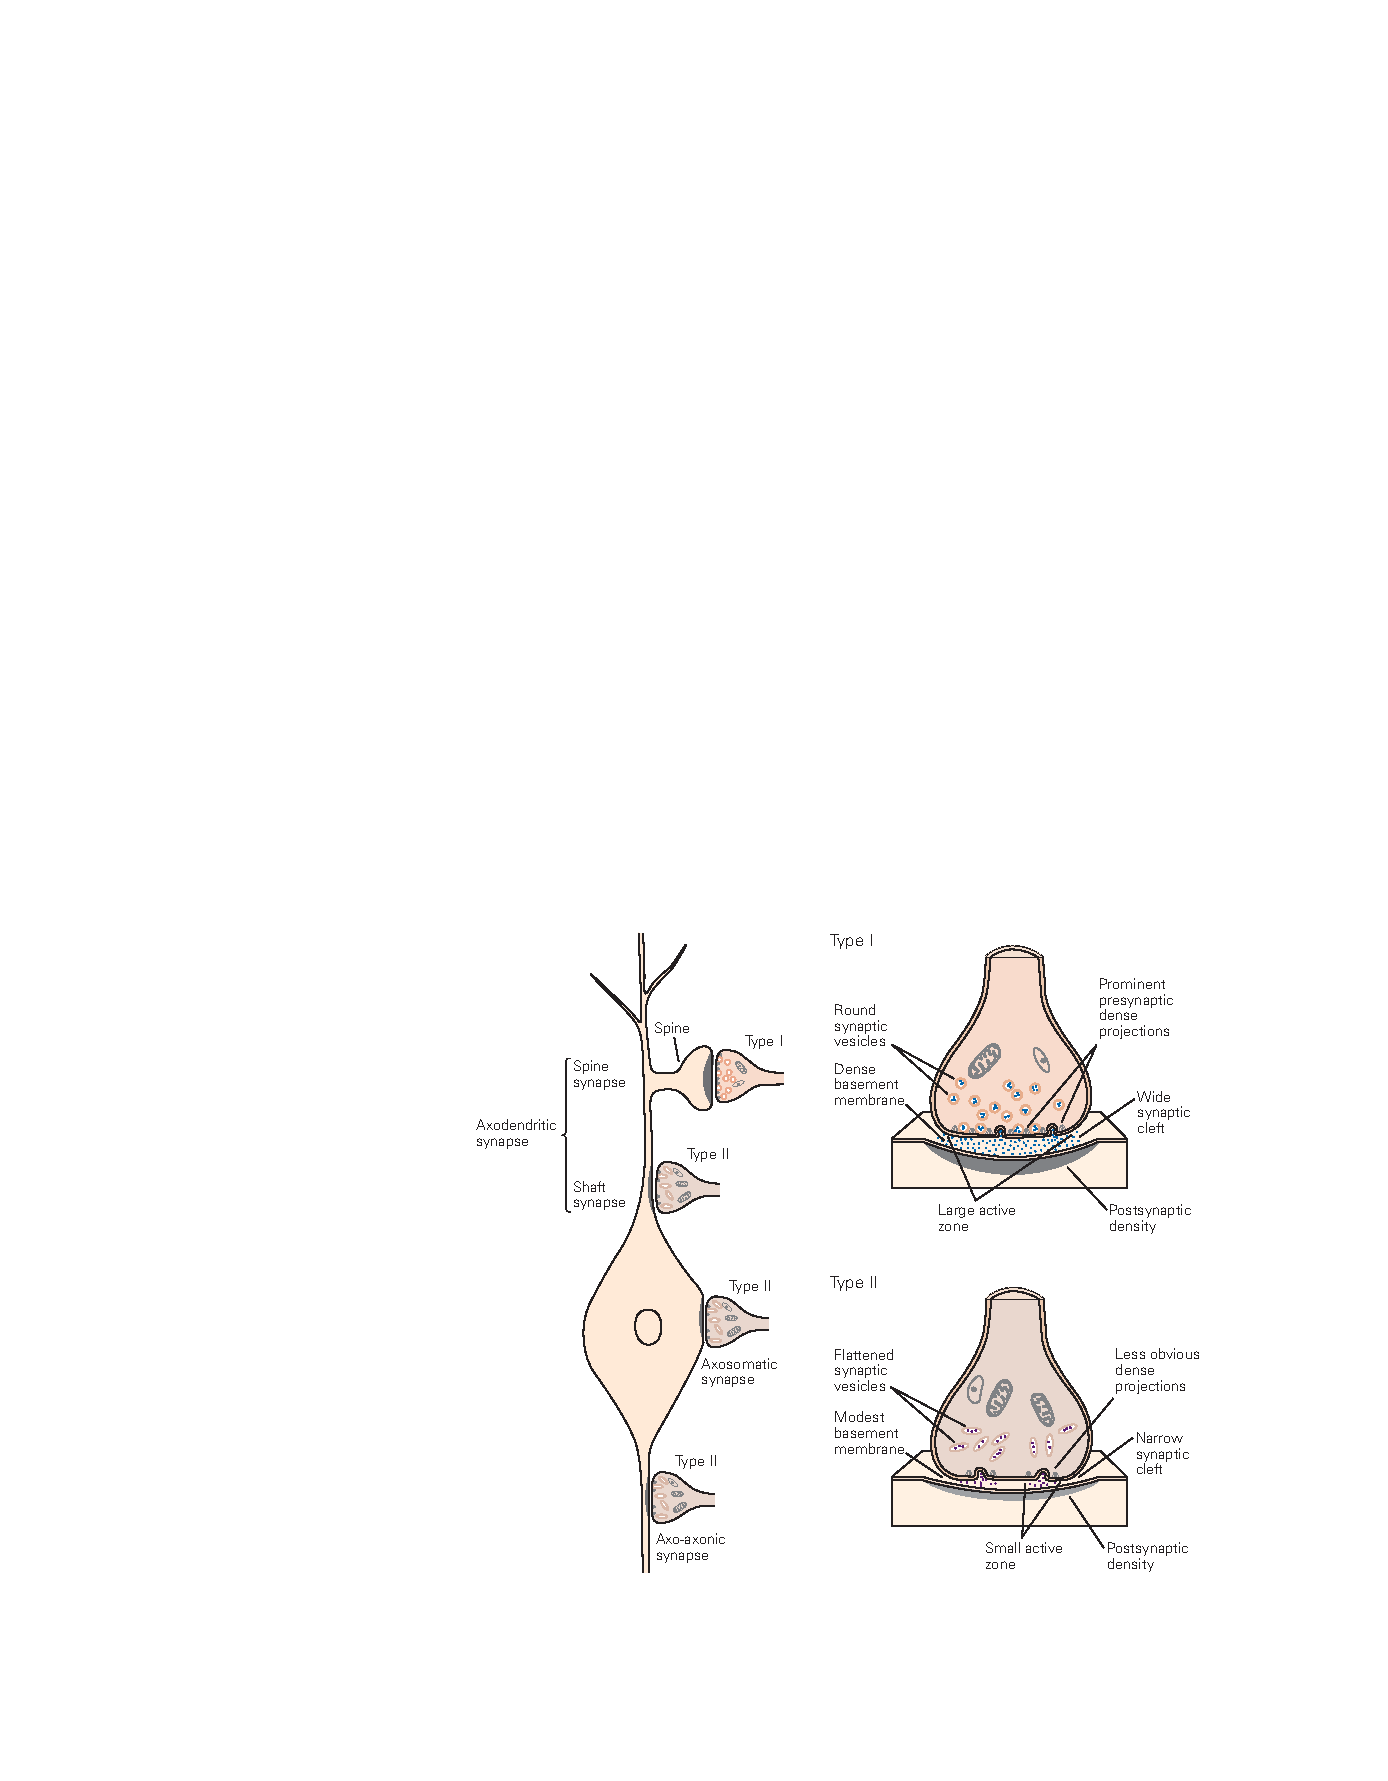
\includegraphics[width=0.8\linewidth]{chap13/fig_13_2}
	\caption{中枢神经系统中两种最常见的突触形态类型是格雷 I 型和 II 型。
		I 型通常是兴奋性的,而 II 型通常是抑制性的。
		差异包括囊泡的形状、突触前密度的突出、活动区的总面积、突触间隙的宽度以及致密基底膜的存在。
		I 型突触通常接触专门的树突投射,称为棘,并且不太常见地接触树突的轴。
		II 型突触接触细胞体 (轴体)、树突轴 (轴-树)、轴突起始段 (轴-轴) 和另一个神经元的突触前末端 (未显示)。}
	\label{fig:13_2}
\end{figure}


虽然树突通常位于突触后,而轴突末端位于突触前,但神经细胞的所有四个区域——轴突、突触前末端、细胞体和树突——都可以是化学突触的突触前或突触后部位。
如图~\ref{fig:13_2}~所示,最常见的接触类型是轴突、轴体和轴突-轴突(按照惯例,首先确定突触前元件)。
兴奋性突触通常是轴突状的,主要发生在树突棘上。
抑制性突触通常形成于树突轴、细胞体和轴突起始段。
还发现了树突状突触和体细胞突触,但它们很少见。


作为一般规则,突触与轴突初始段的接近程度被认为决定了其有效性。
在靠近细胞体的部位产生的给定突触后电流将在轴突起始段的触发区产生更大的膜电位变化,因此对动作电位输出的影响比在更远的部位产生的相同电流更大树突。
这是因为当突触电位传播到细胞体时,一些在远处进入突触后膜的电荷会从树突膜中泄漏出来(第~\ref{chap:chap9}~章)。
一些神经元通过在远端突触放置比近端突触更多的谷氨酸受体来补偿这种影响,确保树突树上不同位置的输入在初始段具有更等效的影响。
与轴突和轴体输入相反,大多数轴突突触对突触后细胞的触发区没有直接影响。
相反,它们通过控制从突触前末梢释放的递质数量来影响神经活动(第~\ref{chap:chap15}~章)。



\section{兴奋性突触传递由可渗透阳离子的离子型谷氨酸受体通道介导}

从牵张受体感觉神经元的突触前末梢释放的兴奋性递质是氨基酸 \textit{L-谷氨酸},它是大脑和脊髓中的主要兴奋性递质。
\textit{埃克尔斯}和他的同事发现,脊髓运动细胞中的\textit{兴奋性突触后电位}是离子型谷氨酸受体通道打开的结果,该通道可渗透 \ce{Na+} 和 \ce{K+}。
这种离子机制类似于第~\ref{chap:chap12}~章中描述的\textit{乙酰胆碱}在神经肌肉接头处产生的机制。
与\textit{乙酰胆碱}受体通道一样,谷氨酸受体通道以几乎相等的渗透性传导 \ce{Na+} 和 \ce{K+}。
因此,流过这些通道的电流的反转电位为 0 毫伏(见图~\ref{fig:12_7})。


谷氨酸受体可分为两大类:离子型受体和代谢型受体(图~\ref{fig:13_3})。 
存在三种主要类型的离子型谷氨酸受体:\textit{$\alpha$-氨基-3-羟基-5-甲基异恶唑-4-丙酸}、红藻氨酸和\textit{N-甲基-D-天冬氨酸},根据激活它们的药理学激动剂的类型命名。
这些受体对拮抗剂也有不同的敏感性。
\textit{N-甲基-D-天冬氨酸}受体被药物\textit{2-氨基-5-膦酰基缬草酸}选择性阻断。
\textit{$\alpha$-氨基-3-羟基-5-甲基异恶唑-4-丙酸}和红藻氨酸受体不受\textit{2-氨基-5-膦酰基缬草酸}的影响,但两者都被药物\textit{6-氰基-7-硝基喹喔啉-2,3-二酮}阻断。
由于这种共同的药理学敏感性,这两种类型有时被称为非\textit{N-甲基-D-天冬氨酸}受体。
\textit{N-甲基-D-天冬氨酸}和非\textit{N-甲基-D-天冬氨酸}受体之间的另一个重要区别是\textit{N-甲基-D-天冬氨酸}受体通道对钙离子具有高度渗透性,而大多数非\textit{N-甲基-D-天冬氨酸}受体则不然。
有几种类型的代谢型谷氨酸受体,其中大部分可以被\textit{反-(1S,3R)-1-氨基-1,3-环戊烷二羧酸}激活。


\begin{figure}[htbp]
	\centering
	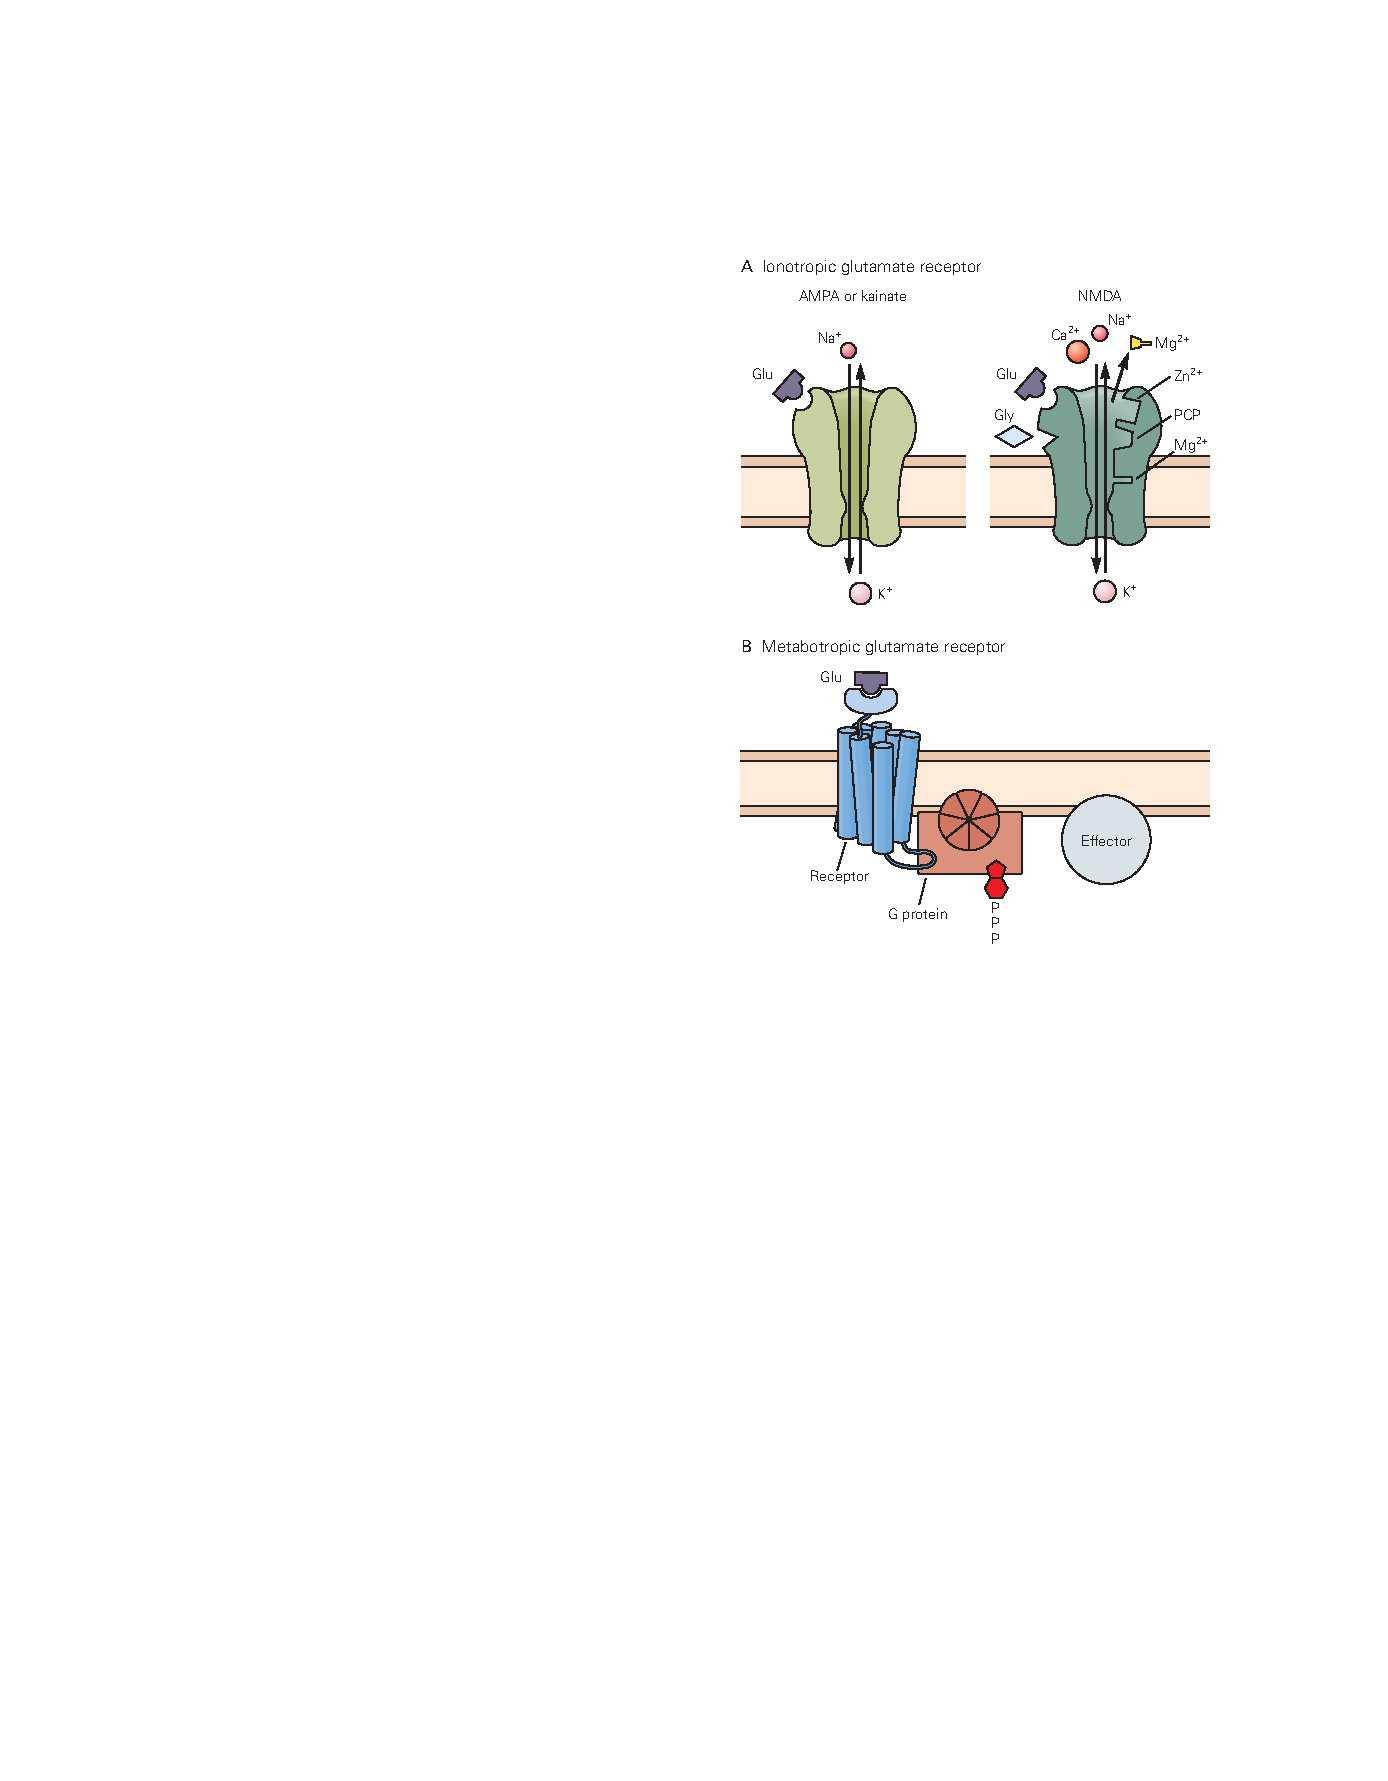
\includegraphics[width=0.55\linewidth]{chap13/fig_13_3}
	\caption{不同类别的谷氨酸受体调节脊髓和大脑神经元中的兴奋性突触动作。
		\textbf{A.} 离子型谷氨酸受体直接门控可渗透阳离子的离子通道。
		\textit{$\alpha$-氨基-3-羟基-5-甲基异恶唑-4-丙酸}和红藻氨酸盐类型分别结合谷氨酸激动剂\textit{$\alpha$-氨基-3-羟基-5-甲基异恶唑-4-丙酸}或红藻氨酸盐;
		这些受体包含一个可渗透 \ce{Na+} 和 \ce{K+} 的通道。\textit{N-甲基-D-天冬氨酸}受体结合谷氨酸激动剂\textit{N-甲基-D-天冬氨酸};
		它包含一个可渗透钙离子、\ce{K+} 和 \ce{Na+} 的通道。
		它具有谷氨酸、甘氨酸、\ce{Zn2+}、\textit{苯环利定}、\textit{佐环平/地卓西平}和 \ce{Mg^2+} 的结合位点,其中每一种都以不同方式调节通道的功能。
		\textbf{B.} \textit{谷氨酸}与代谢型谷氨酸受体的结合通过激活\textit{三磷酸鸟苷结合蛋白}间接门控离子通道,\textit{三磷酸鸟苷结合蛋白}又与效应分子相互作用,从而改变代谢和离子通道活性(第~\ref{chap:chap11} 章)。}
	\label{fig:13_3}
\end{figure}


所有\textit{离子型谷氨酸受体}的作用都是兴奋性或去极化的,因为它们的离子电流的反转电位接近于零,导致通道开放在负膜电位下产生去极化内向电流。
相反,\textit{代谢型受体}可以产生兴奋或抑制,这取决于它们调节的离子电流的逆转电位以及它们是促进通道开放还是通道关闭。



\subsection{离子型谷氨酸受体由一个大基因家族编码}

在过去的 30 年里,已经确定了编码所有主要神经递质受体亚基的多种基因。
此外,这些亚基基因中有许多是可变剪接的,从而产生了更多的多样性。
这种分子分析证明了受体结构之间的进化联系,使我们能够将它们分为三个不同的家族(图~\ref{fig:13_4})。


\begin{figure}[htbp]
	\centering
	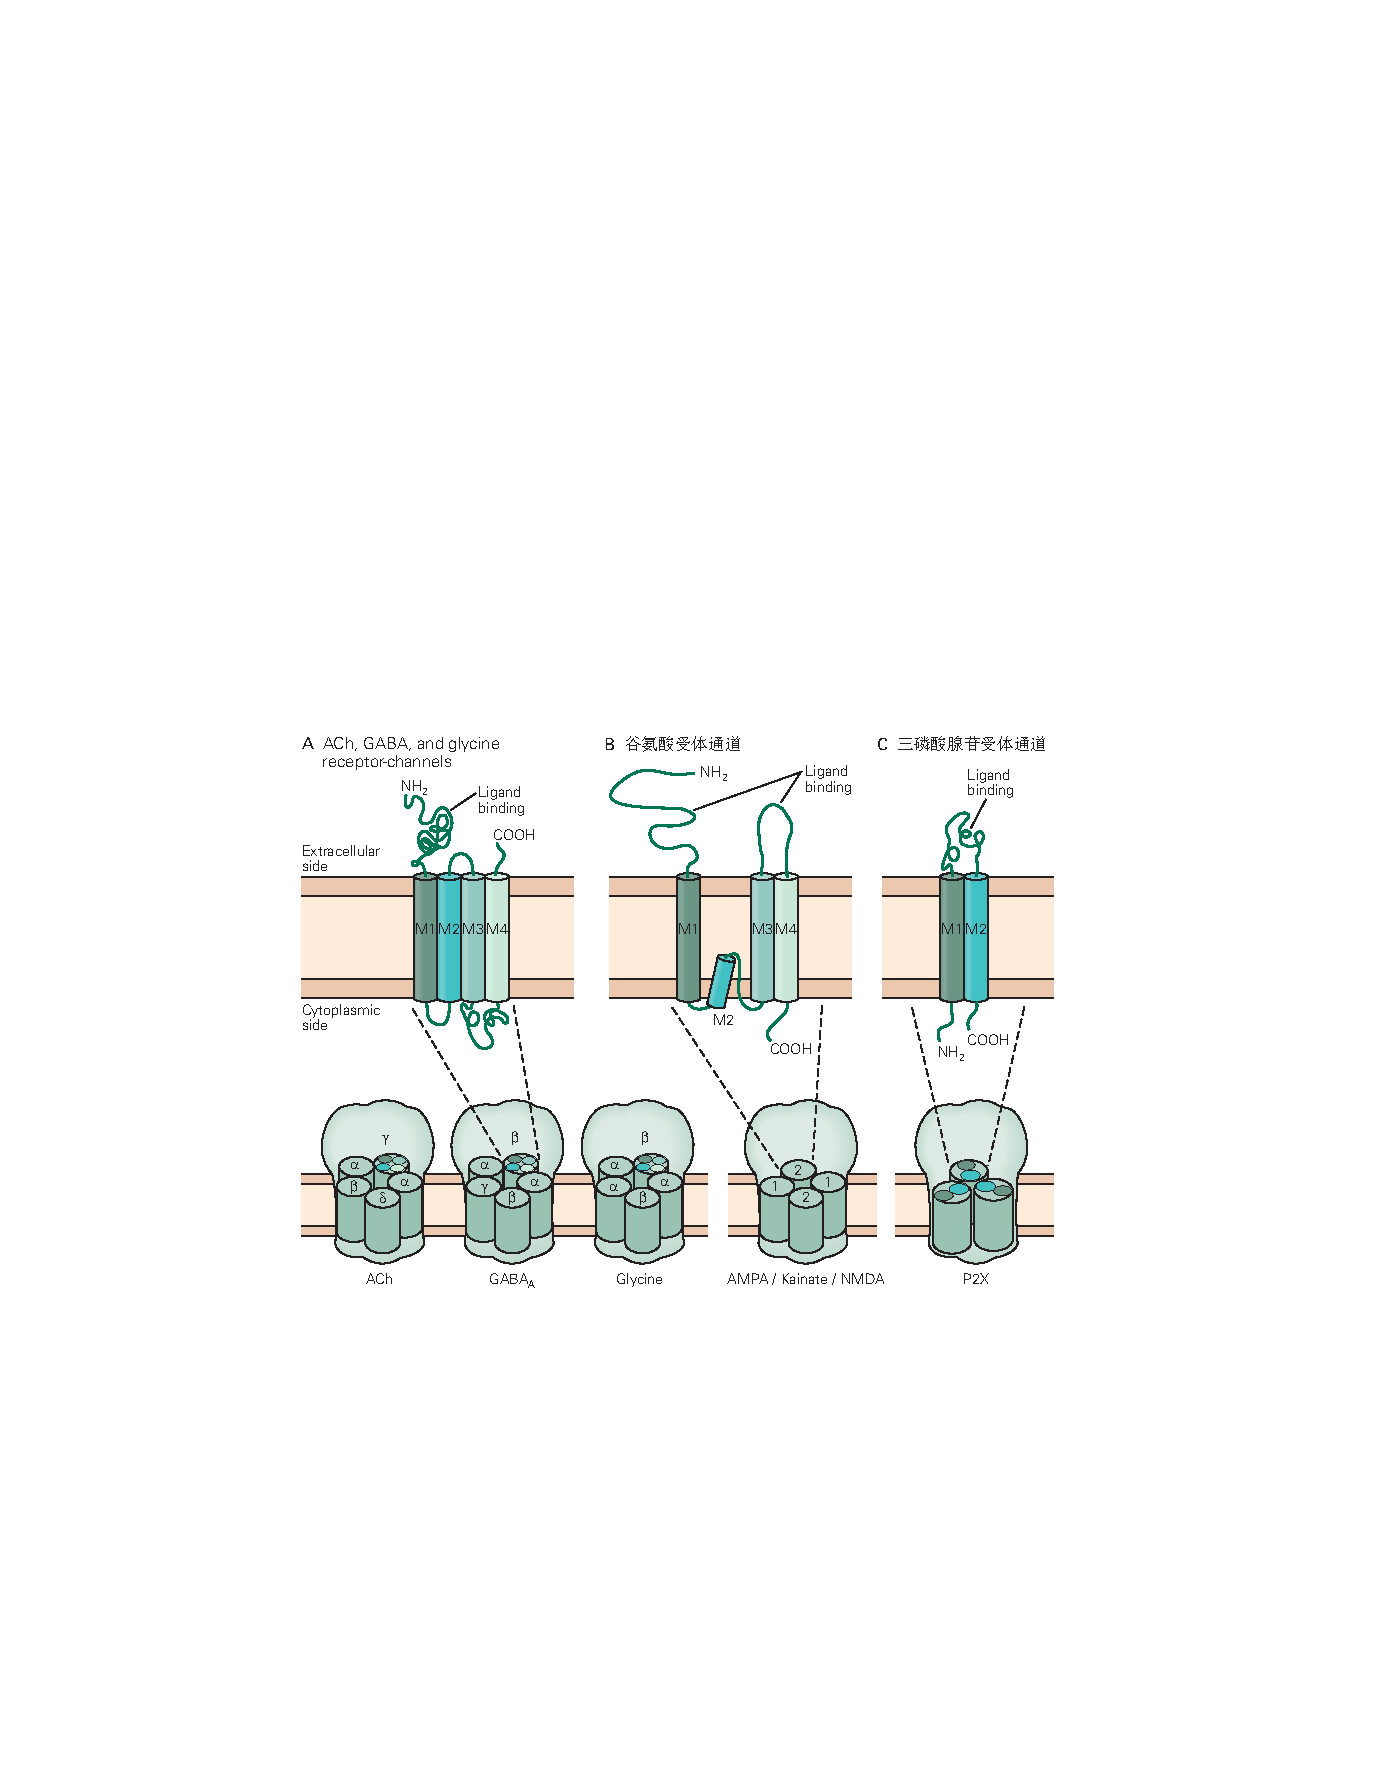
\includegraphics[width=0.75\linewidth]{chap13/fig_13_4}
	\caption{离子型受体的三个家族。
		\textbf{A.} 烟碱\textit{乙酰胆碱}、\textit{$\gamma$氨基丁酸A}和甘氨酸受体通道都是由几种类型的相关亚基组成的五聚体。
		如此处所示,配体结合域由蛋白质的细胞外氨基末端区域形成。
		每个亚基都有一个膜结构域,具有四个跨膜 $\alpha$-螺旋 (M1–M4) 和一个短的细胞外羧基末端。
		M2 螺旋排列通道孔。
		\textbf{B.} 谷氨酸受体通道是四聚体,通常由两种不同类型的密切相关的亚基(此处表示为 1 和 2)组成。
		这些亚基具有一个大的细胞外氨基末端、一个具有三个跨膜 $\alpha$ 螺旋(M1、M3 和 M4)的膜结构域、一个连接 M3 和 M4 螺旋的大细胞外环以及一个细胞内羧基末端。
		M2 部分形成一个环,浸入和浸出膜的细胞质侧,有助于通道的选择性过滤器。
		谷氨酸结合位点由细胞外氨基末端和 M3-M4 细胞外环中的残基形成。
		\textbf{C.} 三磷酸腺苷 (ATP) 受体通道(或嘌呤 P2X 受体)是三聚体。
		每个亚基都具有两个跨膜 $\alpha$ 螺旋(M1 和 M2)和一个结合 ATP 的大细胞外环。 M2 螺旋排列在孔隙中。}
	\label{fig:13_4}
\end{figure}


离子型谷氨酸受体家族包括\textit{$\alpha$-氨基-3-羟基-5-甲基异恶唑-4-丙酸}、红藻氨酸和\textit{N-甲基-D-天冬氨酸}受体。
与编码\textit{N-甲基-D-天冬氨酸}受体的基因相比,编码\textit{$\alpha$-氨基-3-羟基-5-甲基异恶唑-4-丙酸}和红藻氨酸受体的基因彼此之间的关系更为密切。
令人惊讶的是,谷氨酸受体家族与另外两个编码离子型受体的基因家族几乎没有相似之处(其中一个编码烟碱\textit{乙酰胆碱}、\textit{$\gamma$-氨基丁酸}和甘氨酸受体,另一个编码 ATP 受体,如后所述)。


\textit{$\alpha$-氨基-3-羟基-5-甲基异恶唑-4-丙酸}、红藻氨酸和\textit{N-甲基-D-天冬氨酸}受体是由两种或多种类型的相关亚基组成的四聚体,所有四个亚基都排列在一个中心孔周围。
\textit{$\alpha$-氨基-3-羟基-5-甲基异恶唑-4-丙酸}受体亚基由四个独立的基因 (GluA1–GluA4) 编码,而红藻氨酸受体亚基由五个不同的基因 (GluK1–GluK5) 编码。
\textit{$\alpha$-氨基-3-羟基-5-甲基异恶唑-4-丙酸}受体 GluA3 亚基的自身抗体被认为在某些形式的癫痫中发挥重要作用。
这些抗体实际上通过激活含有 GluA3 的受体来模拟谷氨酸,从而导致过度兴奋和癫痫发作。
另一方面,\textit{N-甲基-D-天冬氨酸}受体由一个家族编码,该家族由五个基因组成,分为两组:GluN1 基因编码一种亚基,而四个不同的 GluN2 基因 (A–D) 编码第二种亚基。
每个\textit{N-甲基-D-天冬氨酸}受体包含两个 GluN1 亚基和两个 GluN2 亚基。



\subsection{谷氨酸受体由一组结构模块构成}

所有离子型谷氨酸受体亚基都具有具有相似基序的共同结构。
Eric Gouaux 及其同事对离子型谷氨酸受体的结构提供了重要见解,最初是通过由四个 GluA2 亚基组成的\textit{$\alpha$-氨基-3-羟基-5-甲基异恶唑-4-丙酸}受体的 X 射线晶体学模型。
这些亚基有一个大的细胞外氨基末端结构域,在一级氨基酸序列中紧随其后的是一个细胞外配体结合结构域和一个跨膜结构域(图~\ref{fig:13_4}B~和~\ref{fig:13_5})。
跨膜结构域包含三个跨膜 $\alpha$-螺旋(M1、M3 和 M4)和位于 M1 和 M3 螺旋之间的环 (M2),该环可进出细胞膜的细胞质侧。
这个 M2 环类似于 \ce{K+} 通道的孔隙衬里 P 环,有助于形成通道的选择性过滤器(参见图 8-12)。


\begin{figure}[htbp]
	\centering
	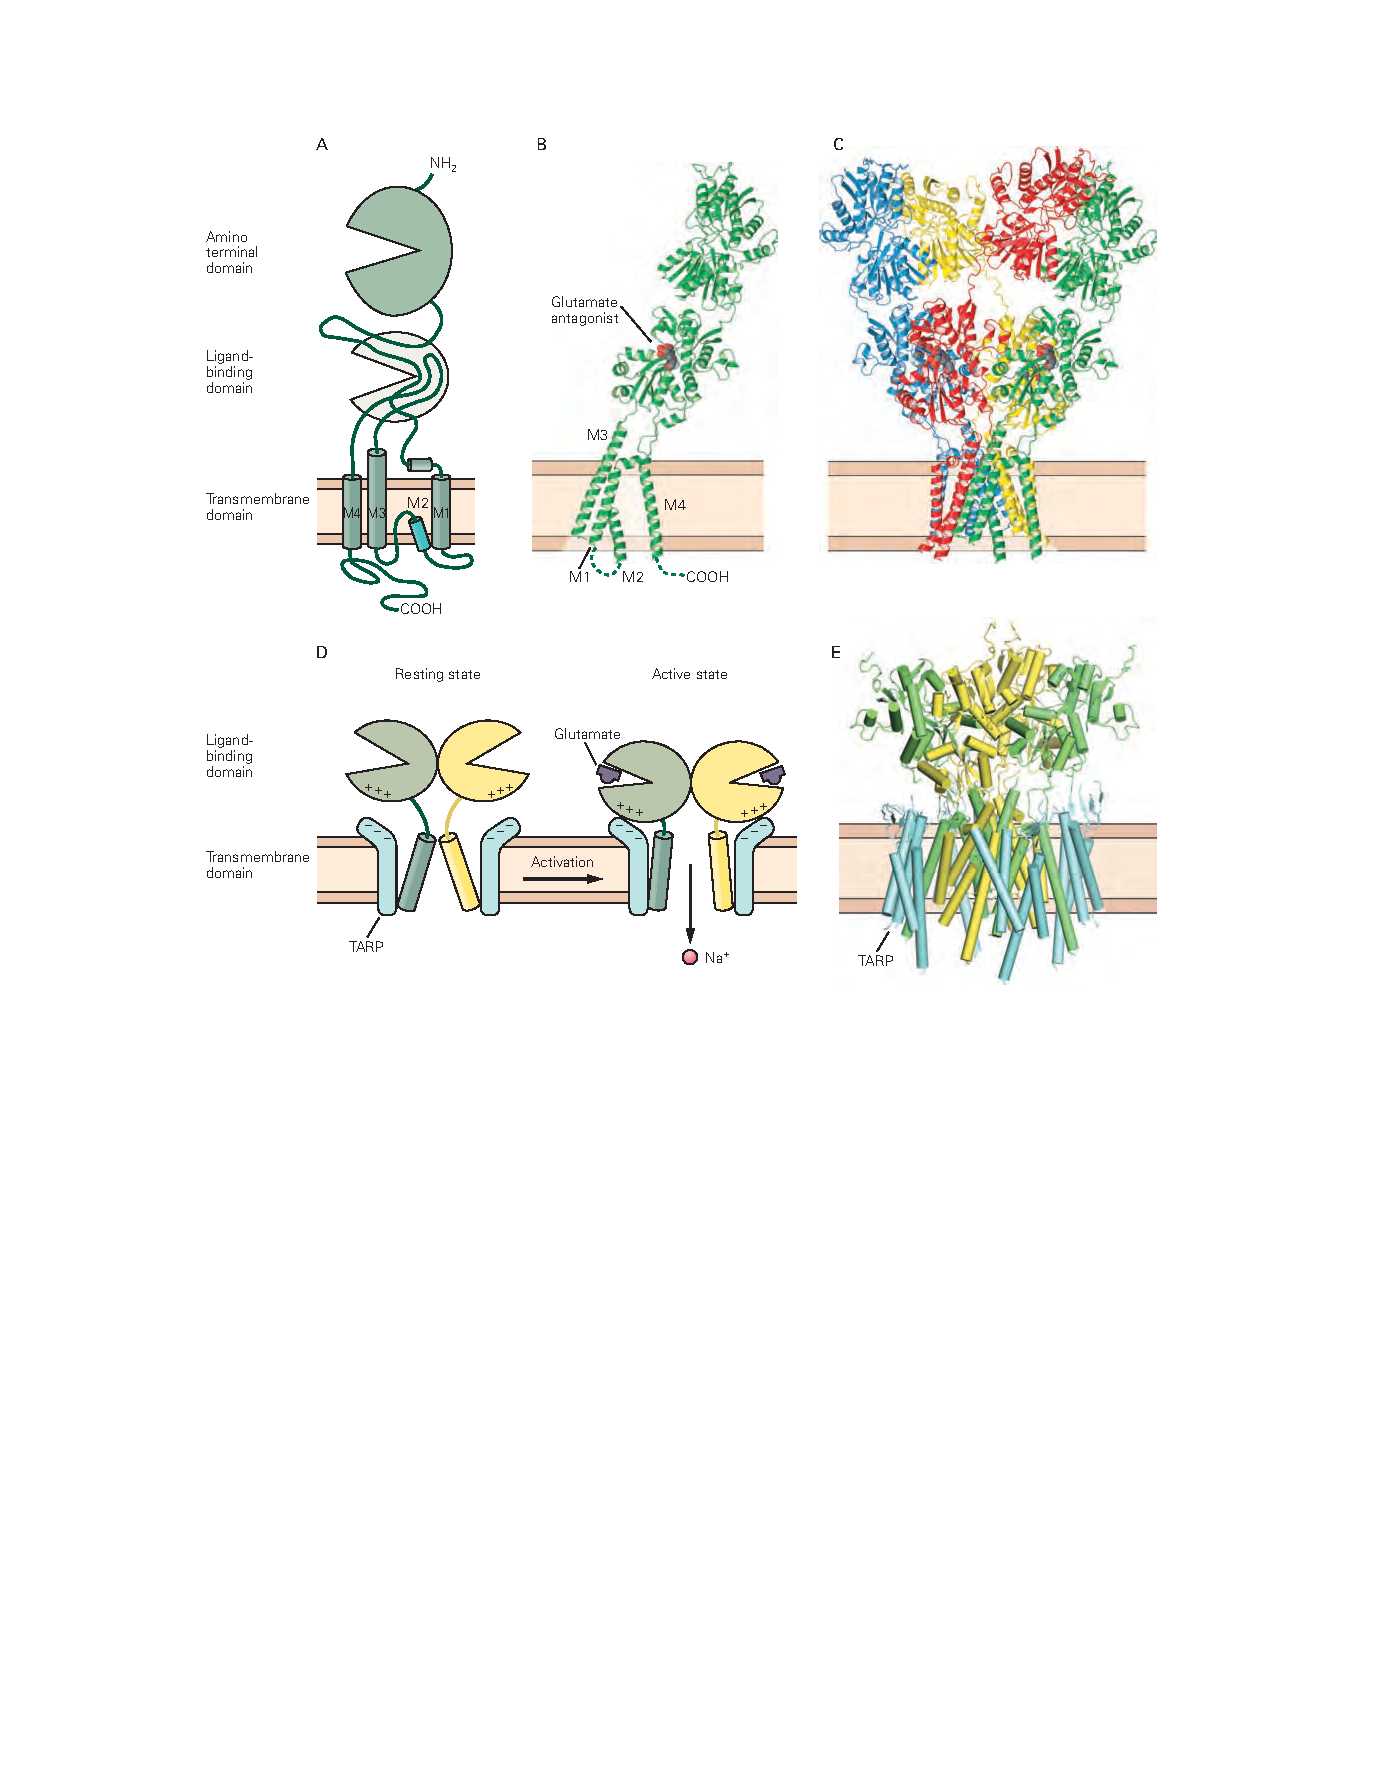
\includegraphics[width=0.8\linewidth]{chap13/fig_13_5}
	\caption{离子型谷氨酸受体的原子结构。
		\textbf{A.} 离子型谷氨酸受体的结构示意图。 
		这些受体包含一个大的细胞外氨基末端、一个包含三个跨膜 $\alpha$螺旋(M1、M3 和 M4)的跨膜结构域,以及一个浸入细胞膜胞质侧的环 (M2)。
		配体结合域由 M1 区段氨基末端侧受体的细胞外区域和连接 M3 和 M4 的细胞外环形成。
		这两个区域交织在一起形成一个蛤壳状结构,结合谷氨酸和各种药理激动剂和竞争性拮抗剂。
		在受体的末端氨基末端形成相似的结构。
		在离子型谷氨酸受体中,这个氨基末端结构域不结合谷氨酸,但被认为可以调节受体功能和突触发育\cite{armstrong1998structure}。
		\textbf{B.} 单个\textit{$\alpha$-氨基-3-羟基-5-甲基异恶唑-4-丙酸}受体 GluA2 亚基的三维 X 射线晶体结构。
		此侧视图显示了氨基末端、配体结合和跨膜结构域(与面板 A 相比)。
		指示了 M1、M3 和 M4 跨膜 $\alpha$-螺旋,以及 M2 环中的短 $\alpha$-螺旋。
		显示了与配体结合域结合的谷氨酸竞争性拮抗剂分子(红色空间填充表示)。
		连接膜 $\alpha$-螺旋的细胞质环未在结构中解析,并绘制为虚线\cite{sobolevsky2009x}。
		\textbf{C.} 此侧视图显示了由四个相同的 GluA2 亚基组装而成的受体的结构(出于说明目的,亚基的颜色不同)。
		这些亚基通过它们的胞外结构域结合成一对二聚体(双重对称)。
		在氨基末端结构域中,一个二聚体由蓝色和黄色亚基形成,另一个二聚体由红色和绿色亚基形成。
		在配体结合域中,亚基改变伙伴。
		在一个二聚体中,蓝色亚基与红色亚基结合,而在另一个二聚体中,黄色亚基与绿色亚基结合。
		在跨膜区域,亚基结合为四重对称四聚体。
		这种极不寻常的亚基排列的意义尚不完全清楚\cite{sobolevsky2009x}。
		\textbf{D.} 与成孔 GluA2 亚基相关的辅助 TARP 亚基(蓝色)的卡通侧视图。
		为简单起见,仅显示了四个 GluA2 亚基中的两个的跨膜和配体结合域。
		还显示了四个 TARP 亚基中的两个。
		谷氨酸的结合导致蛤壳样配体结合域关闭,从而导致打开孔的跨膜域的构象变化。
		TARP 和 GluA2 之间的静电相互作用使受体稳定在开放状态\cite{mayer2016structural}。 
		\textbf{E.} TARP-GluA2 复合物的三维结构。
		$\alpha$-螺旋显示为圆柱体。
		四个 TARP 亚基以蓝色显示。
		GluA2 亚基的跨膜和配体结合域以黄色和绿色显示\cite{mayer2016structural}。}
	\label{fig:13_5}
\end{figure}


两个细胞外结构域都与细菌氨基酸结合蛋白结构域同源。 配体结合域是双叶蛤壳状结构(图~\ref{fig:13_5} A),而氨基末端域与代谢型谷氨酸受体的谷氨酸结合域同源,但不结合谷氨酸。
相反,在离子型谷氨酸受体中,该结构域参与亚基组装、谷氨酸以外的配体对受体功能的调节和/或与其他突触蛋白的相互作用以调节突触发育。


配体结合域由蛋白质线性序列中的两个不同区域形成。
一个区域包括氨基末端结构域的末端直至 M1 跨膜螺旋;
第二个区域由连接 M3 和 M4 螺旋的大细胞外环形成(图~\ref{fig:13_5}A)。
在离子型受体中,蛤壳内谷氨酸分子的结合会触发蛤壳叶的闭合;
竞争性拮抗剂也与翻盖结合,但无法触发翻盖关闭。
这表明与蛤壳闭合相关的构象变化对于打开离子通道很重要。


除了形成受体通道的核心亚基外,\textit{$\alpha$-氨基-3-羟基-5-甲基异恶唑-4-丙酸}受体还包含其他(或辅助)亚基,可调节受体向膜的运输和功能。
一类重要的辅助亚基包括跨膜 \textit{$\alpha$-氨基-3-羟基-5-甲基异恶唑-4-丙酸}受体调节蛋白 (TARP)。
TARP 亚基有四个跨膜结构域,它与成孔\textit{$\alpha$-氨基-3-羟基-5-甲基异恶唑-4-丙酸}受体亚基的结合增强了表面膜运输、突触定位和\textit{$\alpha$-氨基-3-羟基-5-甲基异恶唑-4-丙酸}受体的门控。
第一个被确认的 TARP 家族成员是观星蛋白,它是通过观星突变小鼠的基因筛选分离出来的,之所以这样命名是因为这些动物倾向于将头向后仰并向上凝视。
stargazin 的缺失会导致小脑颗粒细胞的\textit{$\alpha$-氨基-3-羟基-5-甲基异恶唑-4-丙酸}受体完全缺失,从而导致小脑性共济失调和频繁癫痫发作。
TARP 家族的其他成员同样需要\textit{$\alpha$-氨基-3-羟基-5-甲基异恶唑-4-丙酸}受体运输到其他类型神经元的表面膜。


高分辨率冷冻电子显微镜揭示了与\textit{$\alpha$-氨基-3-羟基-5-甲基异恶唑-4-丙酸}受体亚基相关的 TARP 亚基结构(图~\ref{fig:13_5}D,E)。
这些研究表明,TARP 亚基与\textit{$\alpha$-氨基-3-羟基-5-甲基异恶唑-4-丙酸}受体的配体结合域蛤壳之间的相互作用可以使受体稳定在谷氨酸结合的开放状态,从而增强通道开放时间、单通道电导和对谷氨酸的亲和力。


鉴于谷氨酸受体的各种亚型之间的同源性,红藻氨酸和\textit{N-甲基-D-天冬氨酸}受体的整体结构与同源 GluA2 受体的结构相似也就不足为奇了。
然而,有一些重要的差异导致不同受体的不同生理功能。 
\textit{N-甲基-D-天冬氨酸}受体通道对钙离子的高渗透性已定位于成孔 M2 环中的单个氨基酸残基。
所有\textit{N-甲基-D-天冬氨酸}受体亚基在孔中的这个位置都含有中性残基天冬酰胺。
在大多数类型的\textit{$\alpha$-氨基-3-羟基-5-甲基异恶唑-4-丙酸}受体亚基中,该位置的残基是不带电荷的氨基酸谷氨酰胺;
然而,在 GluA2 亚基中,相应的 M2 残基是精氨酸,一种带正电荷的碱性氨基酸。
即使包含一个 GluA2 亚基也会阻止\textit{$\alpha$-氨基-3-羟基-5-甲基异恶唑-4-丙酸}受体通道传导钙离子(图~\ref{fig:13_6}B),这很可能是精氨酸强静电排斥的结果。
缺少 GluA2 亚基的细胞中\textit{$\alpha$-氨基-3-羟基-5-甲基异恶唑-4-丙酸}受体通道的打开会产生显着的钙离子流入,因为这些受体的孔缺乏带正电的精氨酸残基。


\begin{figure}[htbp]
	\centering
	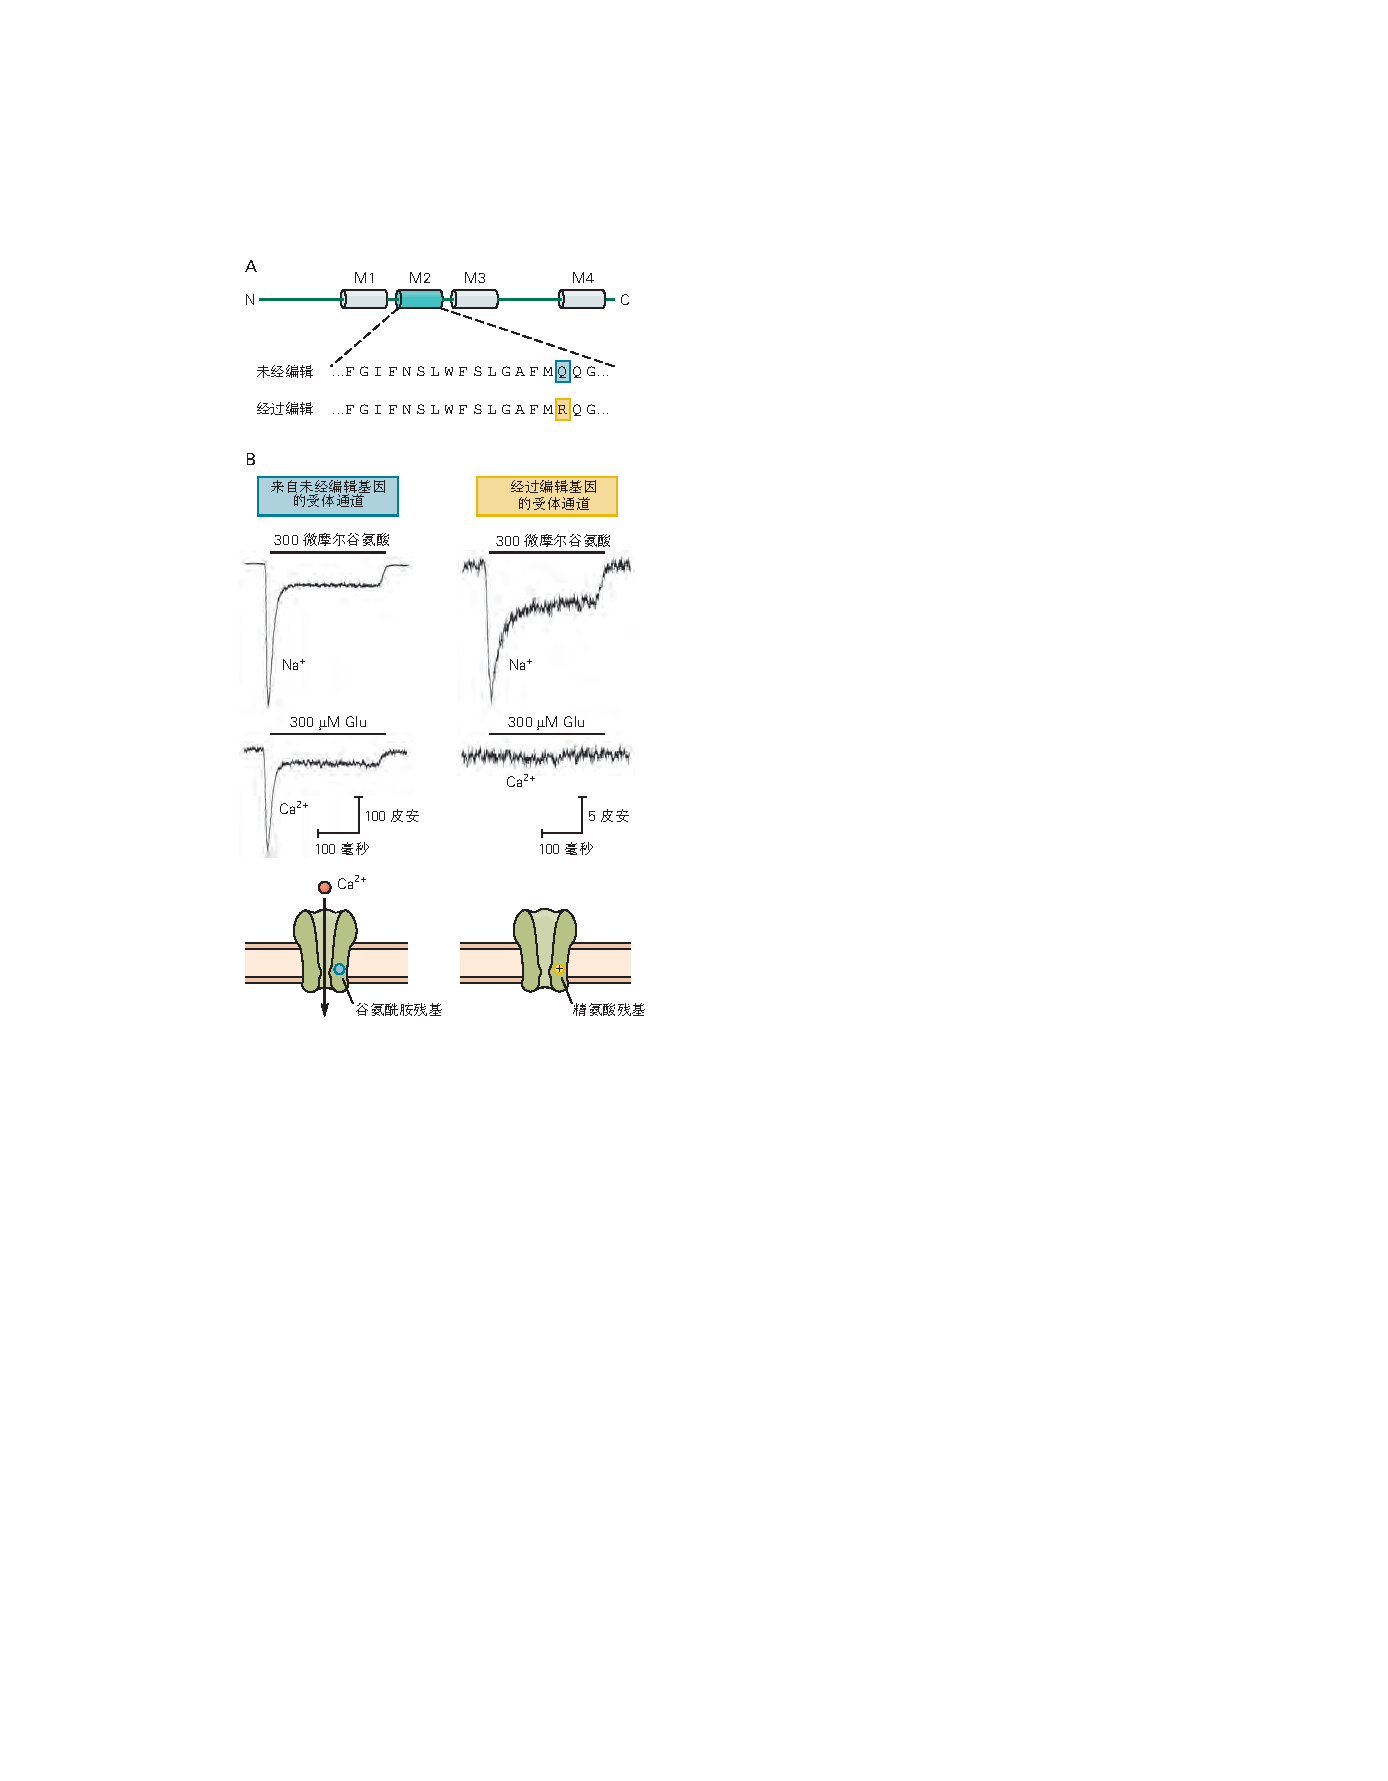
\includegraphics[width=0.45\linewidth]{chap13/fig_13_6}
	\caption{\textit{$\alpha$-氨基-3-羟基-5-甲基异恶唑-4-丙酸}受体通道钙离子渗透性的决定因素。
		\textbf{A.} \textit{核糖核酸}编辑前后GluA2基因编码的\textit{$\alpha$-氨基-3-羟基-5-甲基异恶唑-4-丙酸}受体通道M2区氨基酸序列比较。
		未经编辑的转录本编码极性残基谷氨酰胺(Q,单字母氨基酸符号),而编辑的转录本编码带正电的残基精氨酸 (R)。
		在成人中,GluA2 蛋白几乎完全以经过编辑的形式存在。
		\textbf{B.} 未经编辑的转录物表达的\textit{$\alpha$-氨基-3-羟基-5-甲基异恶唑-4-丙酸}受体通道传导 \ce{Ca^2+}(左迹线),而经编辑的转录物表达的\textit{$\alpha$-氨基-3-羟基-5-甲基异恶唑-4-丙酸}受体通道则不会(右迹线)。
		迹线显示谷氨酸盐以细胞外 \ce{Na+}(顶部)或钙离子(底部)作为主要渗透阳离子引起的电流\cite{sakmann1992nobel}。}
	\label{fig:13_6}
\end{figure}


有趣的是,GluA2 基因的\textit{脱氧核糖核酸}在 M2 环的这个位置不编码精氨酸残基,而是编码谷氨酰胺残基。
转录后,GluA2 \textit{信使核糖核酸}中的谷氨酰胺密码子通过称为\textit{核糖核酸}编辑的酶促过程被替换为精氨酸密码子(图~\ref{fig:13_6}A)。
使用转基因小鼠研究了这种\textit{核糖核酸}编辑的重要性,该小鼠的 GluA2 基因经过工程改造,因此谷氨酰胺密码子中的相关核苷酸不能再变为精氨酸。
这些小鼠在出生后几周内出现癫痫发作并死亡,这可能是因为所有\textit{$\alpha$-氨基-3-羟基-5-甲基异恶唑-4-丙酸}受体的高钙离子渗透性导致细胞内钙离子过量。



\subsection{\textit{N-甲基-D-天冬氨酸}和\textit{$\alpha$-氨基-3-羟基-5-甲基异恶唑-4-丙酸}受体由突触后密度的蛋白质网络组织}

不同的谷氨酸受体是如何在兴奋性突触中定位和排列的? 
与大多数离子型受体一样,谷氨酸受体通常聚集在膜的突触后位点,与谷氨酸能突触前末端正好相反。
成熟神经系统中的绝大多数兴奋性突触同时包含\textit{N-甲基-D-天冬氨酸}和\textit{$\alpha$-氨基-3-羟基-5-甲基异恶唑-4-丙酸}受体,而在早期发育中,仅包含\textit{N-甲基-D-天冬氨酸}受体的突触很常见。
受体在单个突触处的定位和表达模式取决于构成突触后密度并帮助组织突触后细胞膜三维结构的大量调节蛋白。


突触后密度 (PSD) 是一种非常稳定的结构,允许其生化分离、纯化和表征。
完整和分离的 PSD 的电子显微镜研究提供了其结构的惊人详细视图(图~\ref{fig:13_7}A)。 
通过使用金标抗体,可以识别突触后膜的特定蛋白质成分,包括谷氨酸受体的位置和数量。
典型的 PSD 直径约为 350 nm,包含大约 20 个\textit{N-甲基-D-天冬氨酸}受体,它们往往位于 PSD 的中心附近,以及 10 到 50 个\textit{$\alpha$-氨基-3-羟基-5-甲基异恶唑-4-丙酸}受体,它们不太集中。
代谢型谷氨酸受体位于外围,PSD 主要区域之外。
所有三种受体类型都与多种细胞质和膜蛋白相互作用,以确保它们的正确定位(图~\ref{fig:13_7} C)。


\begin{figure}[htbp]
	\centering
	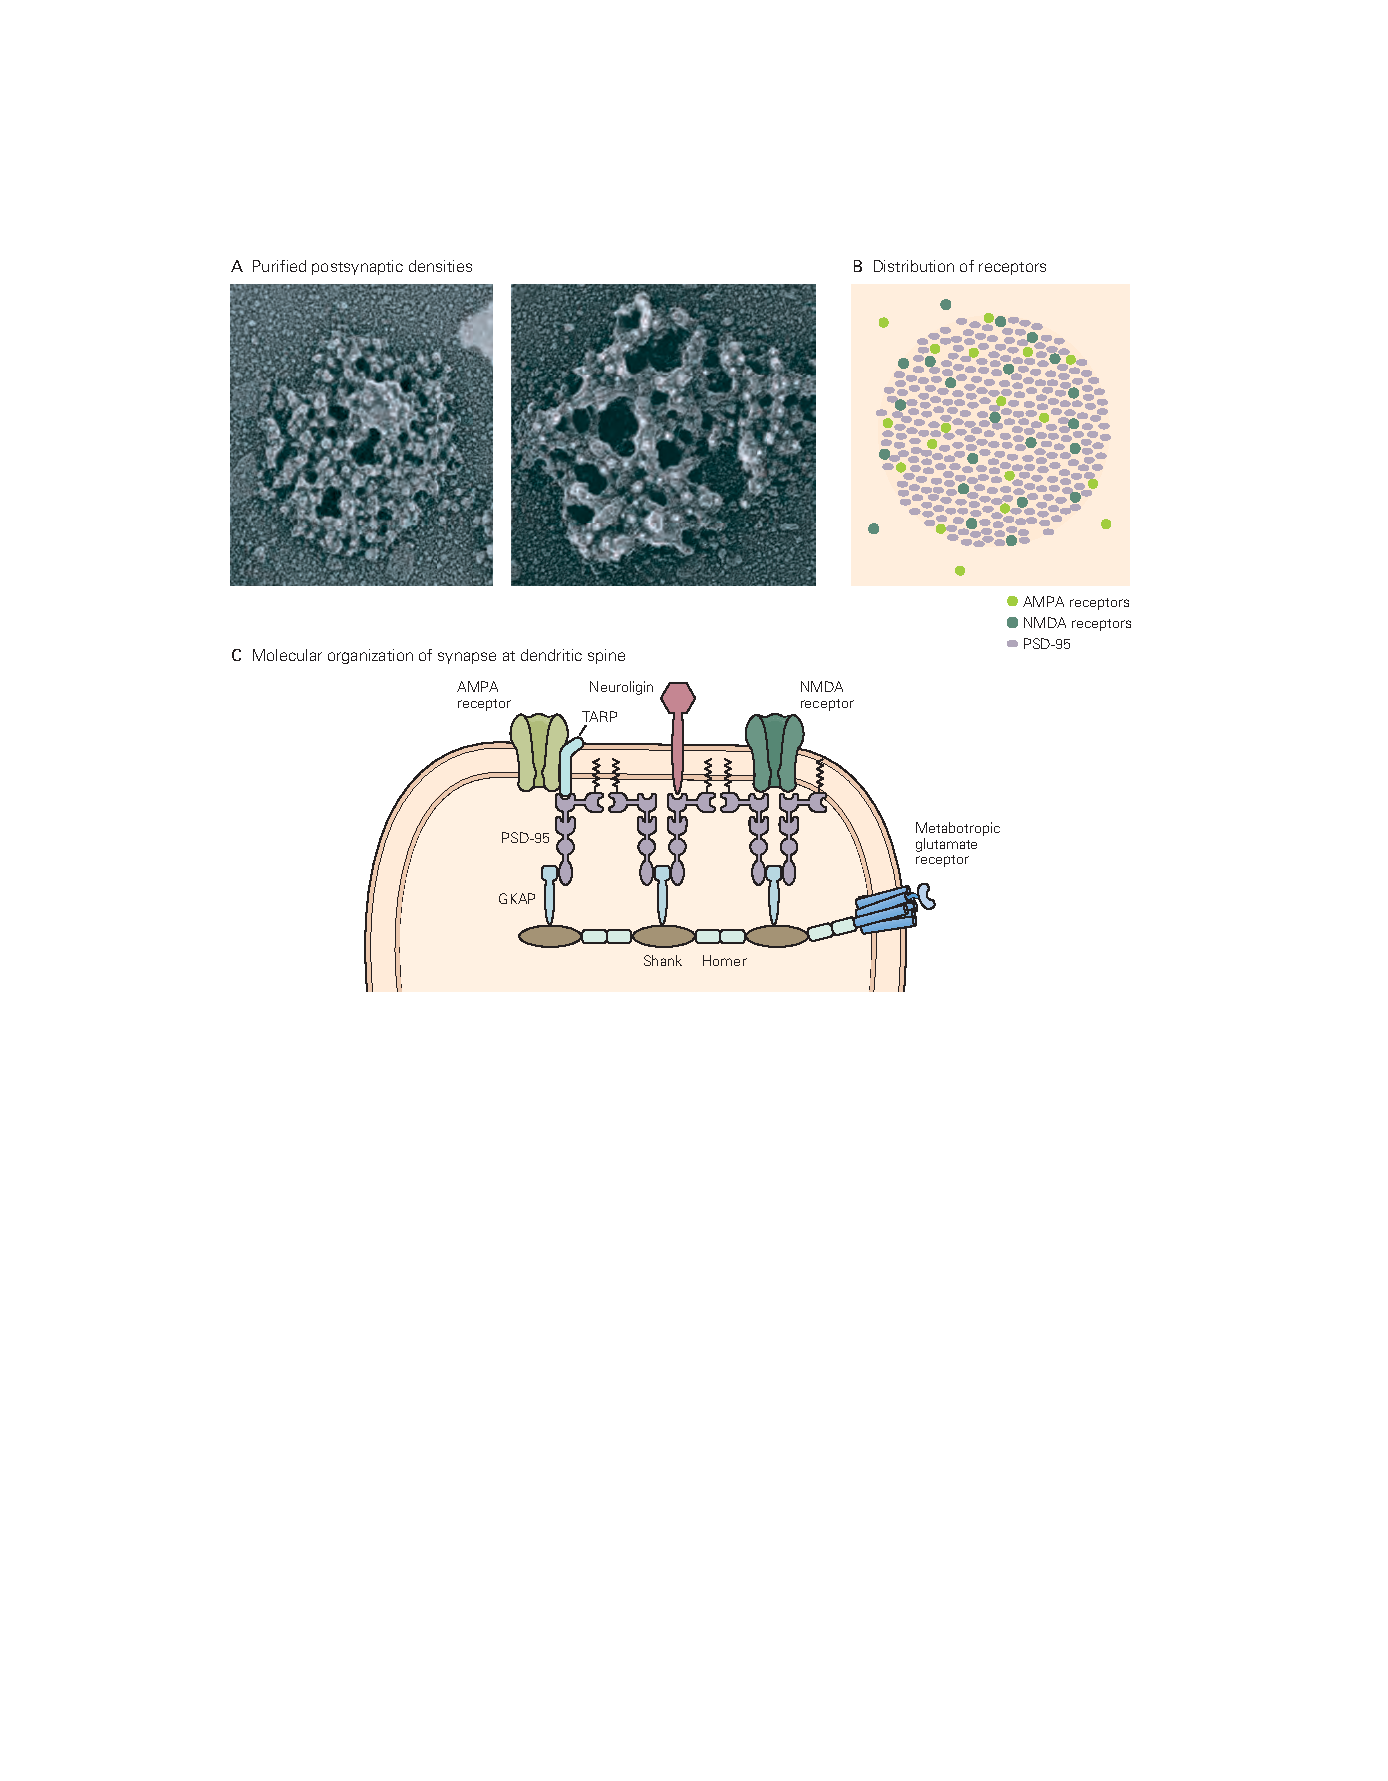
\includegraphics[width=0.7\linewidth]{chap13/fig_13_7}
	\caption{突触后细胞膜在兴奋性突触处组织成大分子复合物。
		含有 PDZ 结构域的蛋白质有助于组织\textit{$\alpha$-氨基-3-羟基-5-甲基异恶唑-4-丙酸}和\textit{N-甲基-D-天冬氨酸}谷氨酸受体在突触后密度的分布\cite{sheng2007postsynaptic}。
		\textbf{A.} 生化纯化的突触后密度的电子显微镜图像,显示蛋白质网络的组织。
		膜脂双层不再存在。
		左图:通常是细胞外部的突触后密度视图。
		该图像由各种受体和膜蛋白的细胞外结构域组成。
		右图:从通常是膜的细胞质侧的突触后密度视图。
		白点显示免疫标记的鸟苷酸激酶锚定蛋白,这是突触后密度的重要组成部分。
		\textbf{B.} NMDA 受体、\textit{$\alpha$-氨基-3-羟基-5-甲基异恶唑-4-丙酸}受体和 PSD-95(一种突出的突触后密度蛋白)在突触处的分布。
		\textbf{C.} 受体网络及其在突触后密度中的相互作用蛋白。
		PSD-95 在其氨基末端包含三个 PDZ 结构域,在其羧基末端包含两个其他蛋白质相互作用基序,一个 SH3 结构域和一个鸟苷酸激酶 (GK) 结构域。
		PSD-95 的某些 PDZ 结构域与 NMDA 受体的 GluN2 亚基的羧基末端结合。
		PSD-95 不直接与\textit{$\alpha$-氨基-3-羟基-5-甲基异恶唑-4-丙酸}受体相互作用,而是与膜蛋白 TARP 家族的羧基末端结合,后者作为辅助亚基与\textit{$\alpha$-氨基-3-羟基-5-甲基异恶唑-4-丙酸}受体相互作用。
		PSD-95 还通过与 GK 相关蛋白 (GKAP) 结合作为各种细胞质蛋白的支架,GK 相关蛋白与 Shank 相互作用,Shank 是一种结合成网状结构的大蛋白,连接突触后密度的各种成分。
		PSD-95 还与 neuroligin 的细胞质区域相互作用。
		代谢型谷氨酸受体位于突触的外围,在那里它与蛋白质 Homer 相互作用,后者又与 Shank 结合。}
	\label{fig:13_7}
\end{figure}


PSD 中对谷氨酸受体聚集很重要的最突出的蛋白质之一是 PSD-95(95 kD 分子量的 PSD 蛋白质)。
PSD-95 是一种膜相关蛋白,包含三个重复区域——所谓的 PDZ 结构域——对蛋白质-蛋白质相互作用很重要。 (PDZ 结构域以首次发现它们的三种蛋白质命名:PSD-95、果蝇中的 DLG 肿瘤抑制蛋白和一种称为 ZO-1 的蛋白质。) 一些蛋白质。
在 PSD-95 中,PDZ 结构域结合\textit{N-甲基-D-天冬氨酸}受体和 Shaker 型电压门控 \ce{K+} 通道,从而将这些通道定位并集中在突触后位点。
PSD-95 还与突触后膜蛋白 neuroligin 相互作用,后者与突触间隙中的突触前膜蛋白 neurexin 相互作用,这是一种对突触发育很重要的相互作用。 neuroligin 的突变被认为是导致某些孤独症病例的原因。


尽管 PSD-95 不直接与\textit{$\alpha$-氨基-3-羟基-5-甲基异恶唑-4-丙酸}受体结合,但它确实与 TARP 亚基相互作用。
\textit{$\alpha$-氨基-3-羟基-5-甲基异恶唑-4-丙酸}受体在突触后膜中的正确定位取决于 TARP 亚基的羧基末端与 PSD-95 之间的相互作用。
\textit{$\alpha$-氨基-3-羟基-5-甲基异恶唑-4-丙酸}受体还与称为 GRIP 的独特 PDZ 结构域蛋白结合,而代谢型谷氨酸受体与另一种称为 Homer 的 PDZ 结构域蛋白相互作用。
除了与受体相互作用外,具有 PDZ 结构域的蛋白质还与许多其他细胞蛋白质相互作用,包括与肌动蛋白细胞骨架结合的蛋白质,从而提供支架,围绕其构建突触后蛋白质复合物。
事实上,对 PSD 的生化分析已经确定了数十种参与\textit{N-甲基-D-天冬氨酸}或\textit{$\alpha$-氨基-3-羟基-5-甲基异恶唑-4-丙酸}受体复合物的蛋白质。



\subsection{N-甲基-D-天冬氨酸受体具有独特的生物物理和药理学特性}

\textit{N-甲基-D-天冬氨酸}受体有几个有趣的特性,可以将其与\textit{$\alpha$-氨基-3-羟基-5-甲基异恶唑-4-丙酸}受体区分开来。
如前所述,\textit{N-甲基-D-天冬氨酸}受体对钙离子具有特别高的渗透性。
此外,\textit{N-甲基-D-天冬氨酸}受体在配体门控通道中是独一无二的,因为它的开放取决于膜电压和递质结合。


电压依赖性是由一种与产生动作电位的电压门控通道所采用的机制完全不同的机制引起的。
在后者中,膜电位的变化通过固有电压传感器转化为通道中的构象变化。
然而,在\textit{N-甲基-D-天冬氨酸}受体中,去极化从通道中移除了外源性栓塞。
在静息膜电位 (−65 毫伏) 下,细胞外 \ce{Mg^2+} 与通道孔隙中的一个位点紧密结合,从而阻断离子电流。
但是,当膜去极化时(例如,通过打开\textit{$\alpha$-氨基-3-羟基-5-甲基异恶唑-4-丙酸}受体通道),\ce{Mg^2+} 通过静电排斥从通道中排出,从而允许 \ce{Na+}、\ce{K+} 和 \ce{Ca^2+} 流动(图~\ref{fig:13_8})。 
\textit{N-甲基-D-天冬氨酸}受体还有一个更有趣的特性,即被致幻剂\textit{苯环利定}和实验化合物\textit{佐环平/地卓西平}抑制。
两种药物都结合到通道孔隙中与 \ce{Mg^2+} 结合位点不同的位点(图~\ref{fig:13_3}A)。


\begin{figure}[htbp]
	\centering
	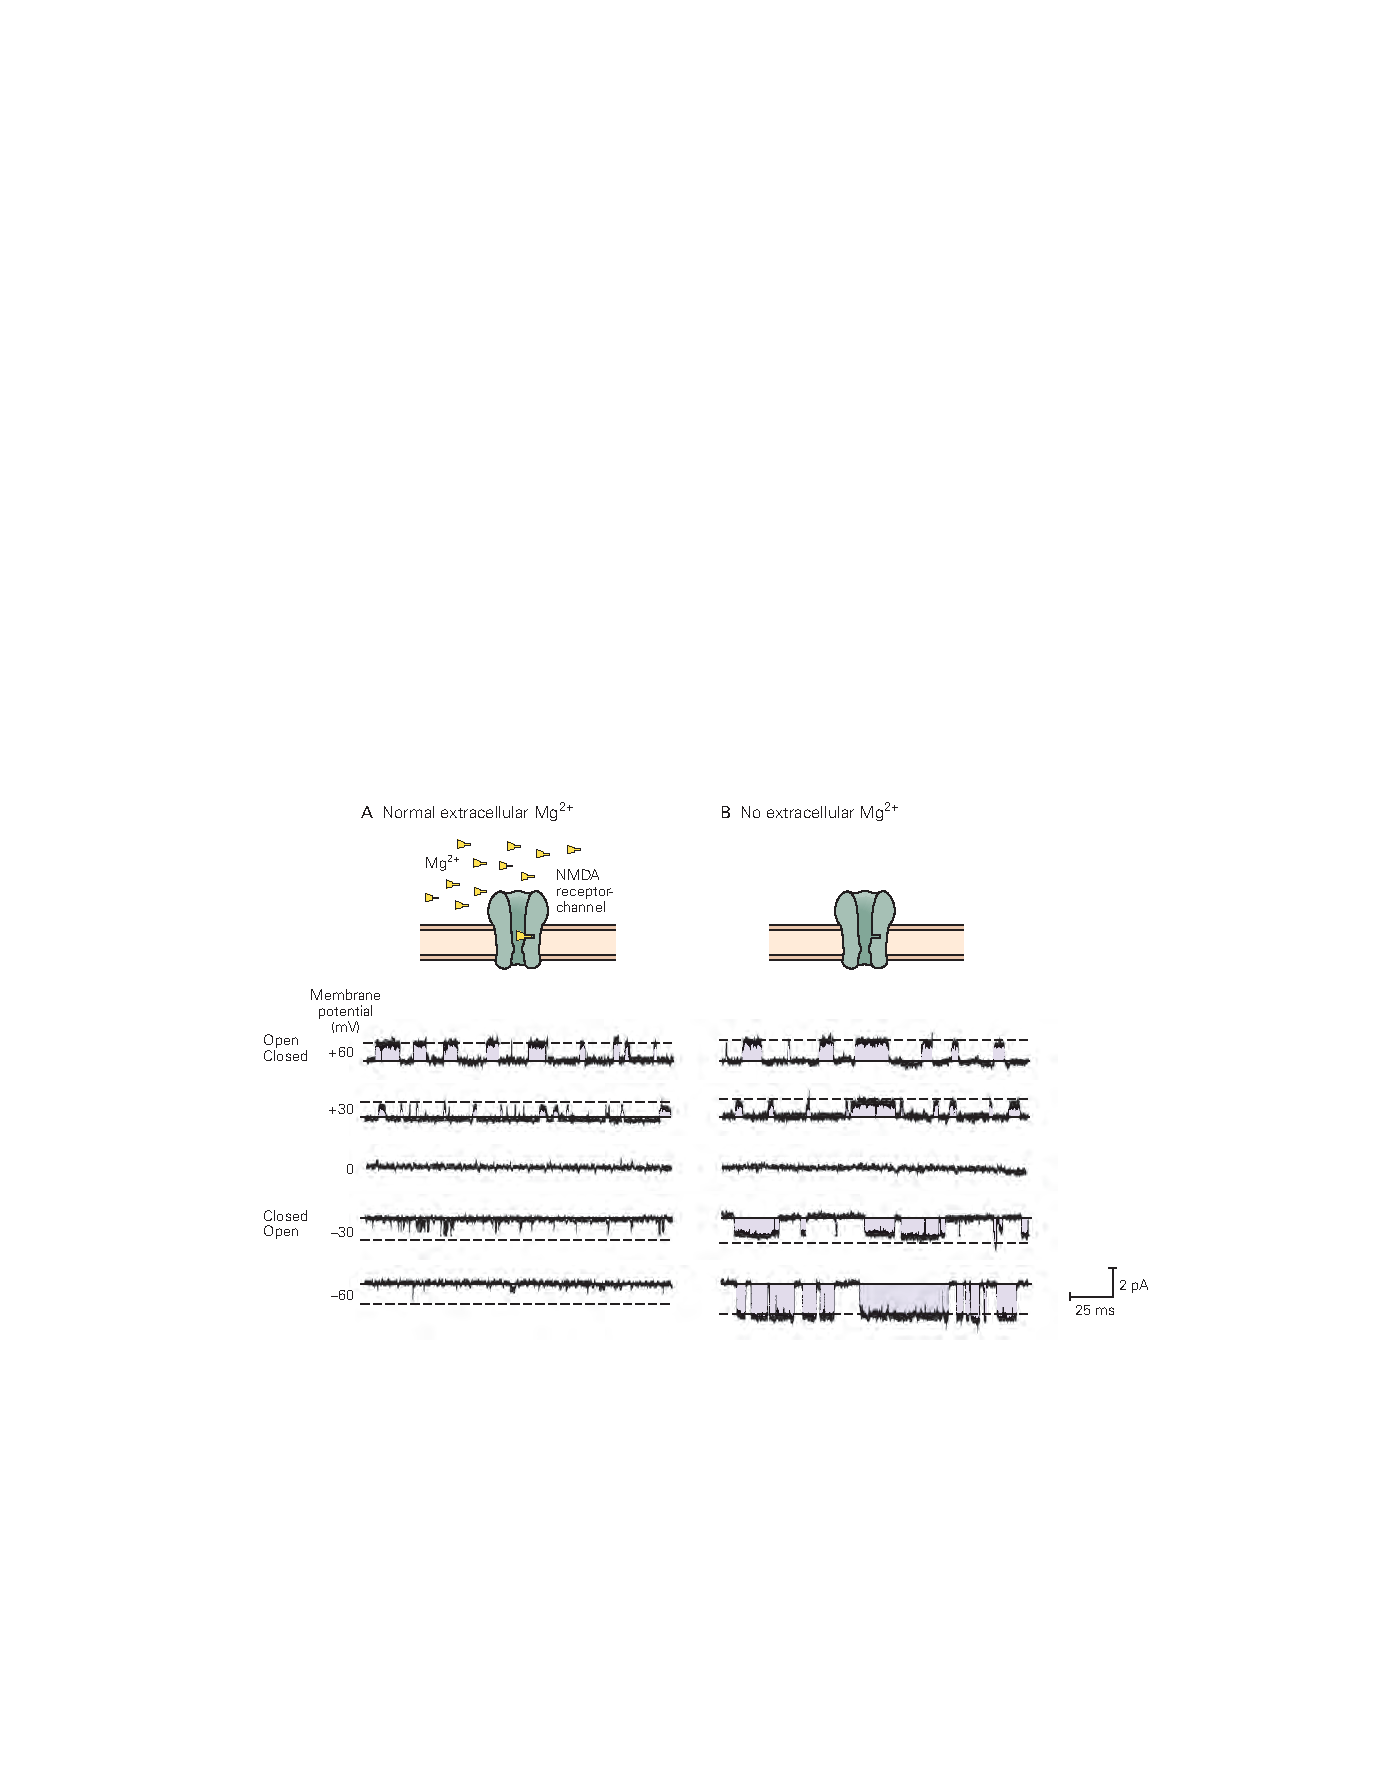
\includegraphics[width=0.8\linewidth]{chap13/fig_13_8}
	\caption{除了谷氨酸之外,单个\textit{N-甲基-D-天冬氨酸}受体通道的打开还取决于膜电位。
		这些膜片钳记录来自单个\textit{N-甲基-D-天冬氨酸}受体通道(来自培养的大鼠海马细胞)。
		向下偏转表示内向(负)电流脉冲; 向上偏转表示向外(正)电流。
		\textbf{A.} 当 \ce{Mg^2+} 以正常浓度存在于细胞外溶液 (1.2 mM) 时,该通道在静息电位 (−60 毫伏) 处大部分被阻断。
		在负膜电位下,由于 \ce{Mg^2+} 阻断,在通道打开时只能看到短暂、闪烁的内向电流。
		对 0 毫伏反转电位(至 +30 毫伏或 +60 毫伏)正电压的大量去极化解除了 \ce{Mg^2+} 阻滞,允许更持久的外向电流脉冲通过通道。
		\textbf{B.} 当 \ce{Mg^2+} 从细胞外溶液中去除时,通道的打开和关闭不依赖于电压。
		通道在 –60 毫伏的静息电位下打开,突触电流在接近 0 毫伏时反转,就像总突触电流一样(参见图~\ref{fig:13_9}B)。}
	\label{fig:13_8}
\end{figure}


\begin{figure}[htbp]
	\centering
	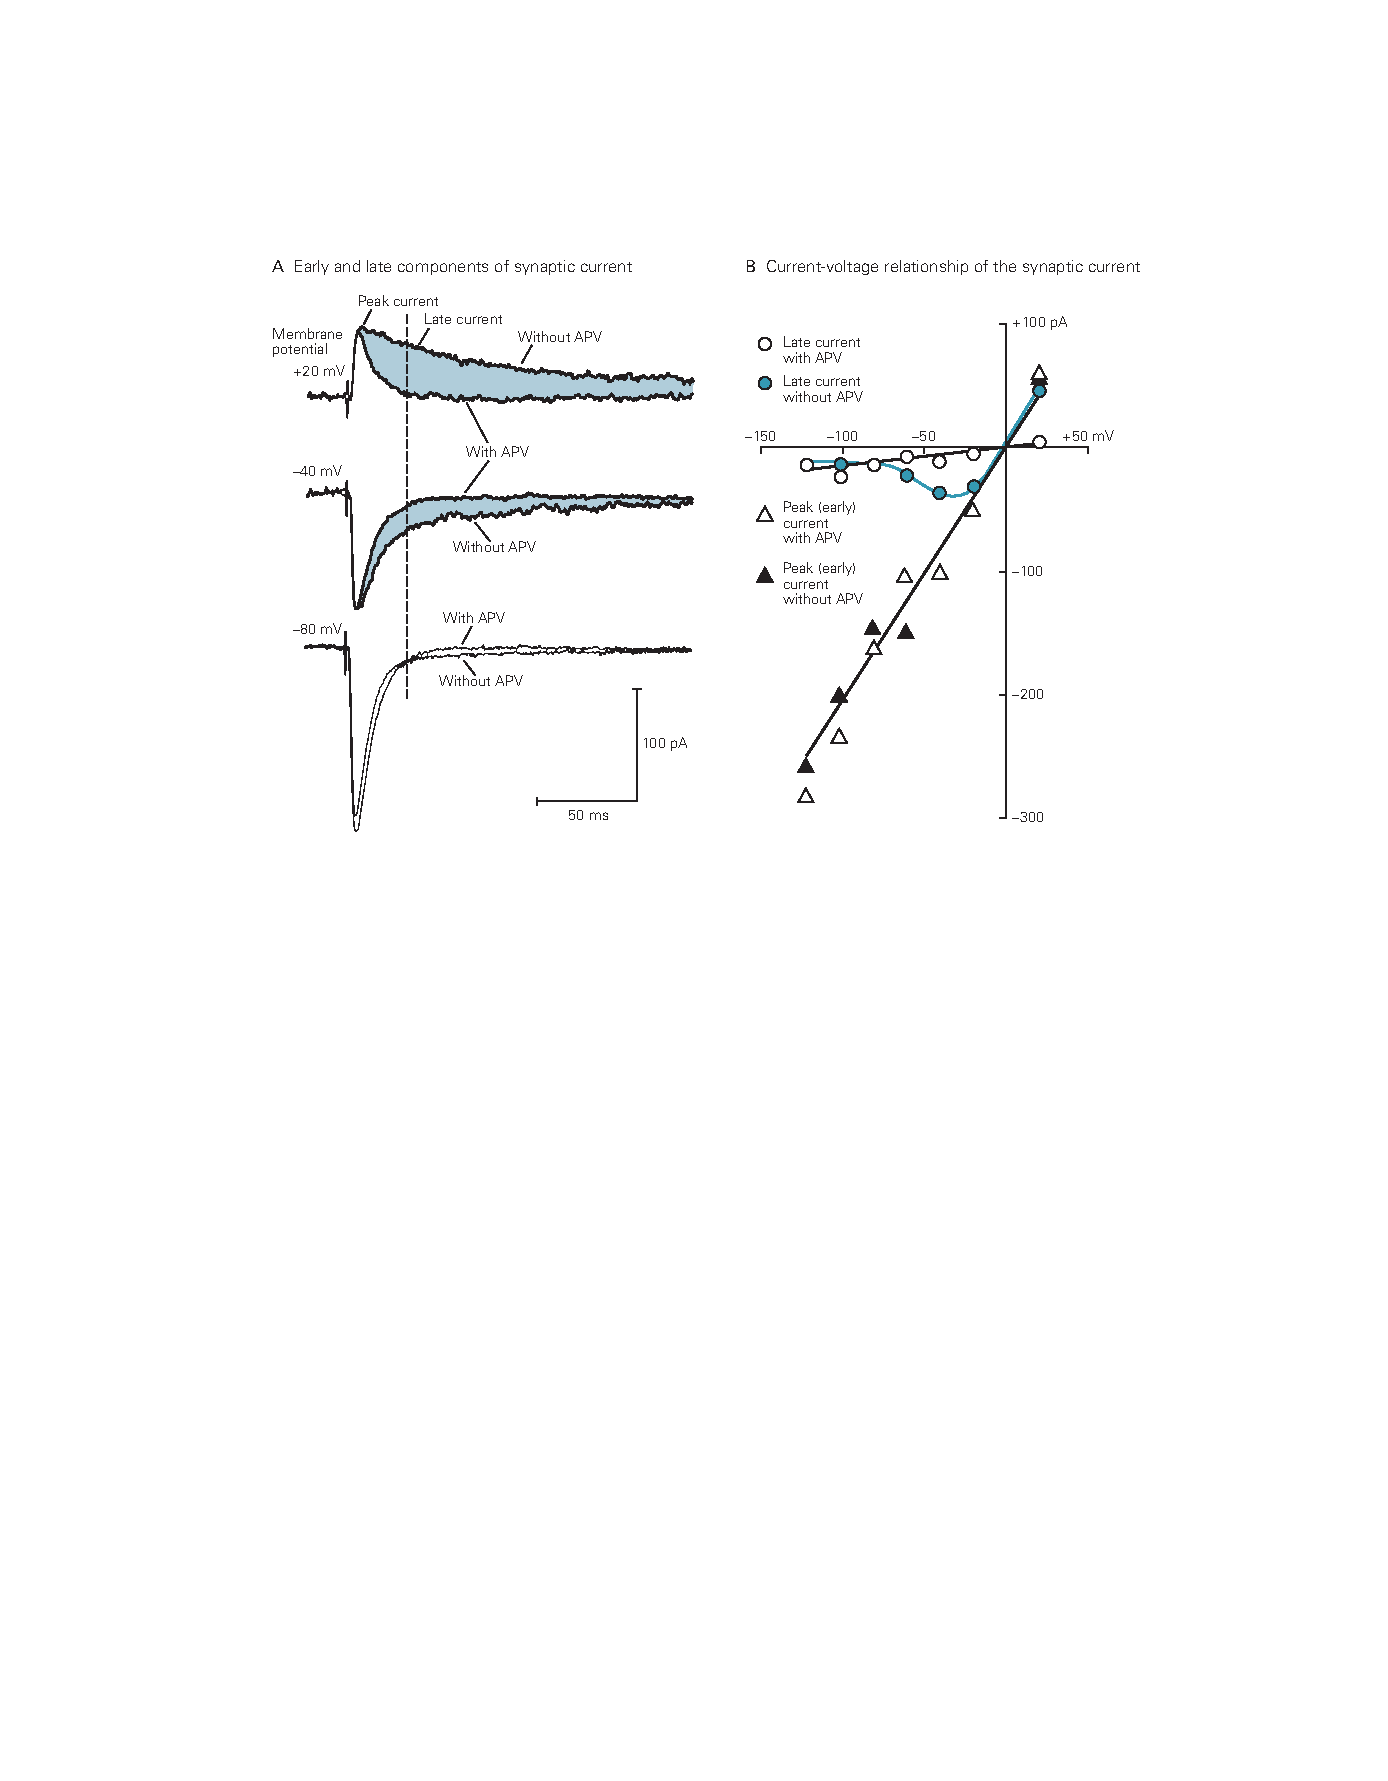
\includegraphics[width=0.75\linewidth]{chap13/fig_13_9}
	\caption{\textit{$\alpha$-氨基-3-羟基-5-甲基异恶唑-4-丙酸}和\textit{N-甲基-D-天冬氨酸}受体通道对兴奋性突触后电流的贡献。 这些电压钳电流记录来自大鼠海马体中的一个细胞。 类似的受体通道存在于运动神经元和整个大脑中\cite{hestrin1990analysis}。
	\textbf{A.} \textit{2-氨基-5-膦酰基缬草酸}药物选择性地结合并阻断 NMDA 受体。
	这里显示的是在三种不同的膜电位下应用 50 μM \textit{2-氨基-5-膦酰基缬草酸}之前和期间的兴奋性突触后电流 (EPSC)。
	痕迹(蓝色区域)之间的差异代表 NMDA 受体通道对 EPSC 的贡献。 在存在\textit{2-氨基-5-膦酰基缬草酸}的情况下保持的电流是\textit{$\alpha$-氨基-3-羟基-5-甲基异恶唑-4-丙酸}受体通道的贡献。
	在 −80 毫伏时,由于明显的 \ce{Mg^2+} 阻滞,没有电流通过 NMDA 受体通道(参见图 \ref{fig:13_8})。
	在 -40 毫伏时,通过 NMDA 受体通道的小的晚期内向电流是明显的。 
	在 +20 毫伏时,晚期分量更为突出并已反转为外向电流。
	突触电流峰值后 25 毫秒的时间(虚线)用于计算 B.B 部分中的晚期电流。
	通过 NMDA 和\textit{$\alpha$-氨基-3-羟基-5-甲基异恶唑-4-丙酸}受体通道的突触后电流在对膜电位的依赖性方面有所不同。
	通过\textit{$\alpha$-氨基-3-羟基-5-甲基异恶唑-4-丙酸}受体通道的电流有助于突触电流的早期阶段(实心三角形)。
	早期阶段是在突触电流的峰值处测量的,并在此处绘制为膜电位的函数。
	通过 NMDA 受体通道的电流有助于突触电流的后期(实心圆)。
	后期阶段是在突触电流峰值后 25 毫秒测量的,此时\textit{$\alpha$-氨基-3-羟基-5-甲基异恶唑-4-丙酸}受体成分几乎衰减到零(参见 A 部分)。
	请注意,\textit{$\alpha$-氨基-3-羟基-5-甲基异恶唑-4-丙酸}受体通道表现为简单的电阻器; 电流和电压呈线性关系。
	相比之下,通过 NMDA 受体通道的电流是非线性的,并且随着膜从 -80 到 -40 毫伏去极化而增加,这是由于 \ce{Mg^2+} 阻滞的逐渐缓解。
	两种受体通道类型的逆转电位均为 0 毫伏。
	存在 50 微米\textit{2-氨基-5-膦酰基缬草酸}时突触电流的分量由未填充的圆圈和三角形表示。
	请注意\textit{2-氨基-5-膦酰基缬草酸}如何阻断 EPSC 的晚期(NMDA 受体)成分而不是早期(\textit{$\alpha$-氨基-3-羟基-5-甲基异恶唑-4-丙酸} 受体)成分。}
	\label{fig:13_9}
\end{figure}


在大多数谷氨酸能中央突触中,突触后膜包含\textit{N-甲基-D-天冬氨酸}和\textit{$\alpha$-氨基-3-羟基-5-甲基异恶唑-4-丙酸}受体。
通过\textit{N-甲基-D-天冬氨酸}和\textit{$\alpha$-氨基-3-羟基-5-甲基异恶唑-4-丙酸}受体的电流对总兴奋性突触后电流 (EPSC) 的相对贡献可以在电压钳实验中使用药理学拮抗剂进行量化(图~\ref{fig:13_9})。
由于\textit{N-甲基-D-天冬氨酸}受体在大多数神经元的正常静息电位下主要被 \ce{Mg^2+} 抑制,因此 EPSC 主要由流经\textit{$\alpha$-氨基-3-羟基-5-甲基异恶唑-4-丙酸}受体的电荷决定。
该电流具有非常快速的上升和衰减阶段。
然而,当神经元去极化并且 \ce{Mg^2+} 被驱出\textit{N-甲基-D-天冬氨酸}受体的口时,更多的电荷流过它们。
因此,当满足两个条件时,\textit{N-甲基-D-天冬氨酸}受体通道最大程度地传导电流:存在谷氨酸,并且细胞去极化。
也就是说,\textit{N-甲基-D-天冬氨酸}受体充当分子“巧合检测器”,在突触前和突触后细胞同时激活时打开。
此外,由于其配体门控的内在动力学,通过\textit{N-甲基-D-天冬氨酸}受体通道的电流上升和衰减的时间进程比通过\textit{$\alpha$-氨基-3-羟基-5-甲基异恶唑-4-丙酸}受体通道的电流慢得多。
因此,\textit{N-甲基-D-天冬氨酸}受体有助于 EPSC 和\textit{兴奋性突触后电位}的晚期、缓慢期。


由于大多数谷氨酸能突触都含有能够自行触发动作电位的\textit{$\alpha$-氨基-3-羟基-5-甲基异恶唑-4-丙酸}受体,那么\textit{N-甲基-D-天冬氨酸}受体的功能是什么?
乍一看,这些受体的功能更加令人费解,因为它们的内在通道通常在静息电位时被 \ce{Mg^2+} 阻断。
然而,\textit{N-甲基-D-天冬氨酸}受体通道对 \ce{Ca^2+} 的高渗透性赋予它们产生细胞内 [\ce{Ca^2+}] 显着升高的特殊能力,从而激活各种钙依赖性信号级联反应,包括几种不同的蛋白激酶(第 ~\ref{chap:chap15}~和~\ref{chap:chap53}~章)。
因此,\textit{N-甲基-D-天冬氨酸}受体激活可以将电信号转化为生化信号。
其中一些生化反应通过称为长期突触可塑性的一系列过程导致突触强度的长期变化,这对于在早期发育过程中完善突触连接和调节成人大脑中的神经回路(包括长期关键回路)非常重要-长期记忆。



\subsection{N-甲基-D-天冬氨酸受体的特性是长期突触可塑性的基础}

1973 年,Tim Bliss 和 Terje Lomo 发现短暂的高强度和高频突触刺激(称为破伤风)会导致海马体中兴奋性突触传递的\textit{长时程增强},海马体是大脑的一个区域 许多形式的长期记忆需要哺乳动物的大脑(图~\ref{fig:13_10};见第~\ref{chap:chap53}~和~\ref{chap:chap54}~章)。
随后的研究表明,\textit{长时程增强}需要通过\textit{N-甲基-D-天冬氨酸}受体通道流入 \ce{Ca^2+},而 NMDA 受体通道会在强直刺激期间响应谷氨酸释放和强烈的突触后去极化的联合作用而打开。
如果在阻断\textit{N-甲基-D-天冬氨酸}受体的\textit{2-氨基-5-膦酰基缬草酸}存在的情况下递送破伤风,或者如果突触后神经元被注射螯合细胞内 \ce{Ca^2+} 的化合物,则\textit{长时程增强}被阻断。


\begin{figure}[htbp]
	\centering
	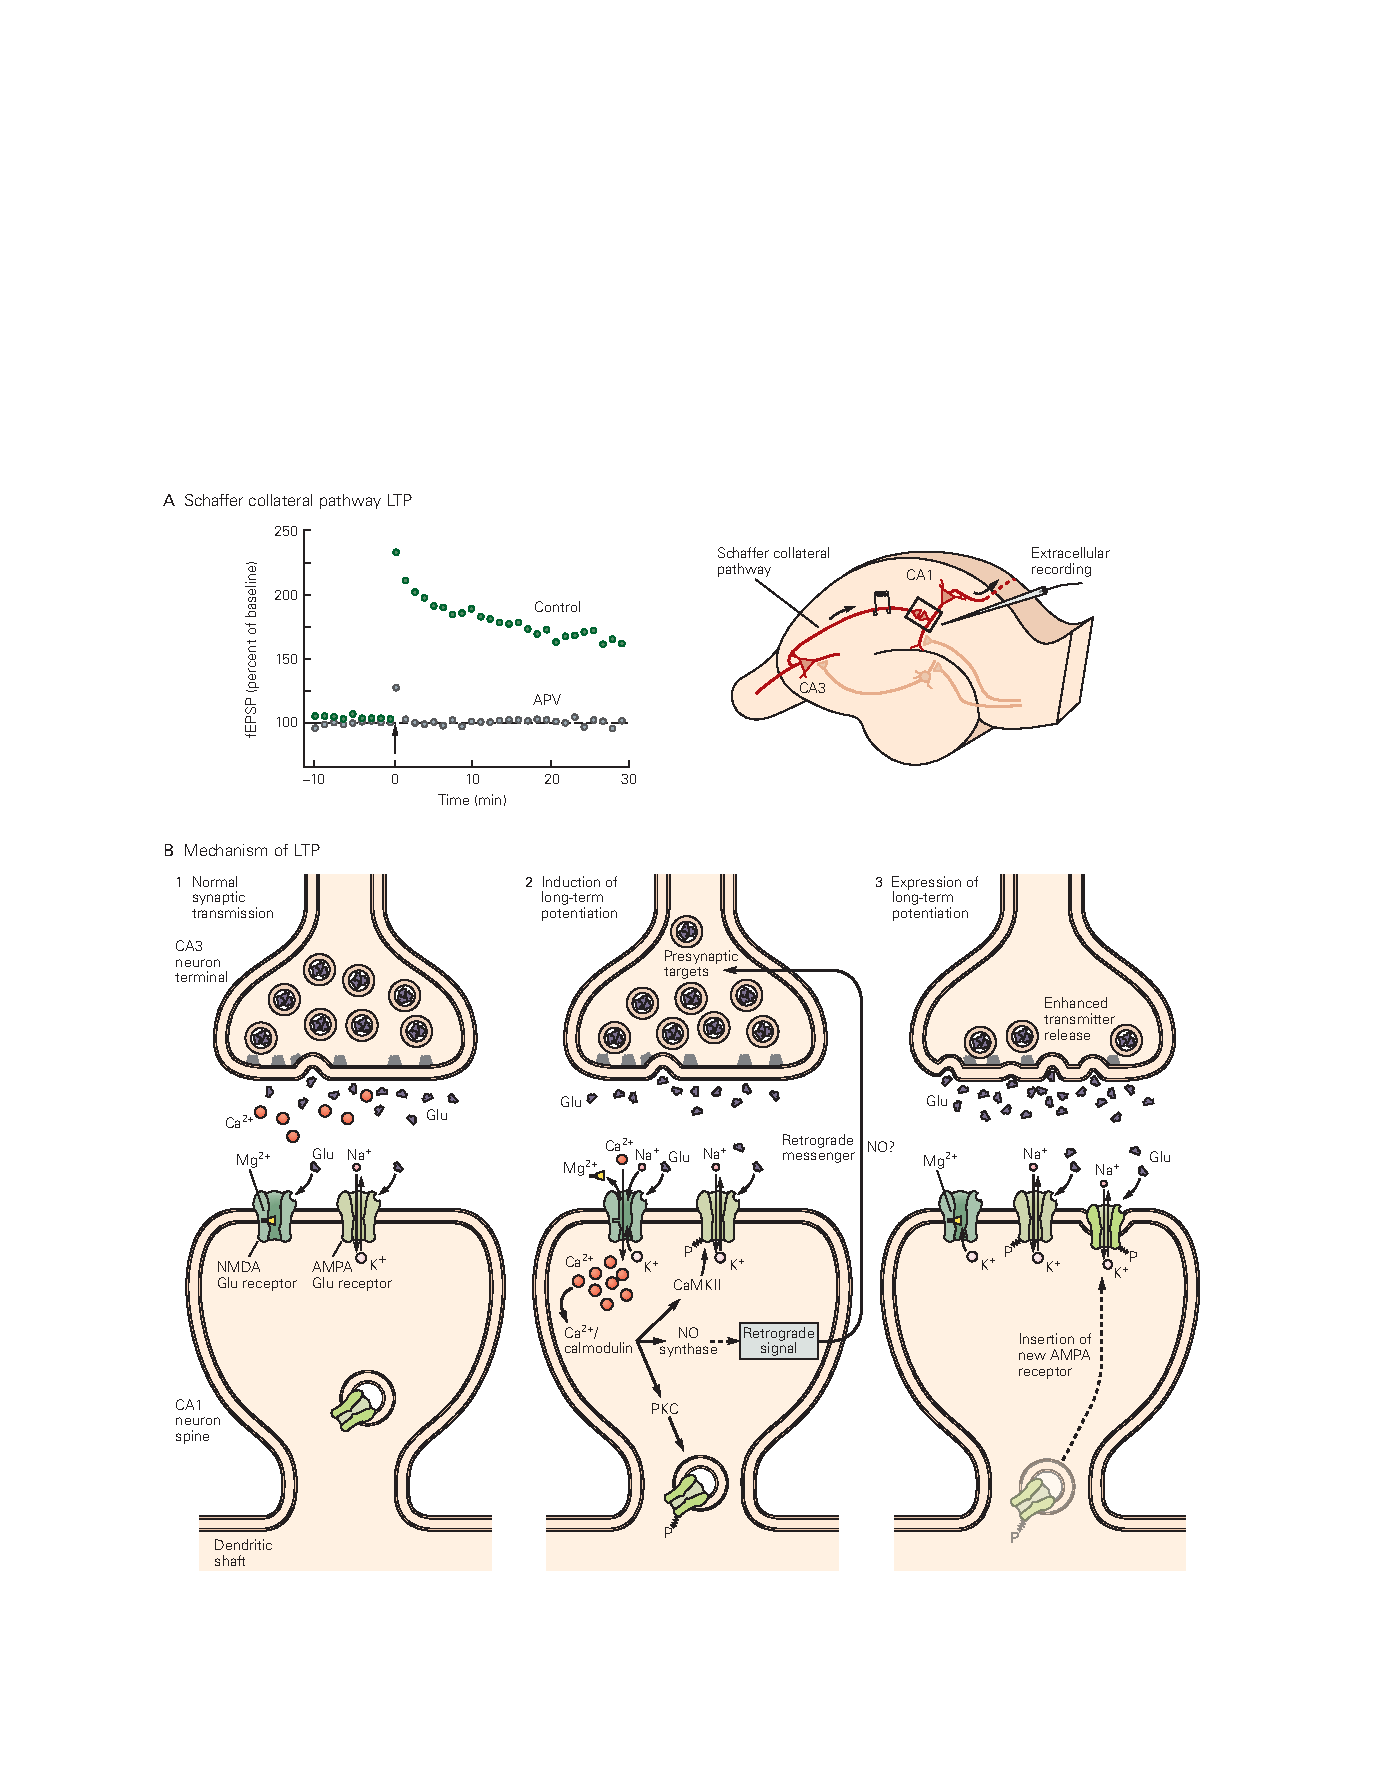
\includegraphics[width=0.85\linewidth]{chap13/fig_13_10}
	\caption{(对面)\textit{N-甲基-D-天冬氨酸}受体依赖性长期增强\textit{谢弗侧支}突触的突触传递。
		\textbf{A.} \textit{谢弗侧支}通路的破伤风刺激 1 秒(箭头)在 CA3 锥体神经元的突触前末梢和 CA1 锥体神经元的突触后树突棘之间的突触处诱导\textit{长时程增强}。
		该图显示突触反应(细胞外场\textit{兴奋性突触后电位}或\textit{场兴奋性突触后电位})的大小占\textit{长时程增强}诱导前初始反应的百分比。
		在这些突触处,\textit{长时程增强}需要激活 CA1 神经元中的\textit{N-甲基-D-天冬氨酸}受体通道; 
		当在\textit{N-甲基-D-天冬氨酸}受体拮抗剂\textit{2-氨基-5-膦酰基缬草酸}存在下递送破伤风时,\textit{长时程增强}被完全阻断\cite{morgan2001electrical}。
		\textbf{B.} \textit{谢弗侧支}突触长时程增强机制模型。
		1. 在正常的低频突触传递过程中,从 CA3 \textit{谢弗侧支}轴突末端释放的谷氨酸 (Glu) 与突触后 CA1 神经元中的 NMDA 和\textit{$\alpha$-氨基-3-羟基-5-甲基异恶唑-4-丙酸}受体结合(特别是在树突棘的突触后膜,兴奋性部位) 输入)。
		钠离子和钾离子流经\textit{$\alpha$-氨基-3-羟基-5-甲基异恶唑-4-丙酸}受体但不流经 NMDA 受体通道,因为它们的孔在负膜电位下被 \ce{Mg^2+} 阻塞。
		2. 在高频破伤风期间,突触后膜的大量去极化(由大量谷氨酸释放导致\textit{$\alpha$-氨基-3-羟基-5-甲基异恶唑-4-丙酸}受体强烈激活引起)解除了 NMDA 受体通道的 \ce{Mg^2+} 阻断,使 \ce{Ca^2+}、\ce{Na+} 和 \ce{K+} 流经这些渠道。
		树突棘中 \ce{Ca^2+} 的增加会激活钙依赖性蛋白激酶——钙/钙调蛋白依赖性激酶 (CaMKII) 和蛋白激酶 C (PKC)——从而诱导\textit{长时程增强}。
		3. 在诱导\textit{长时程增强}期间激活的第二信使级联对突触传递有两个主要影响。
		通过激活蛋白激酶(包括 PKC)进行的磷酸化增强了通过\textit{$\alpha$-氨基-3-羟基-5-甲基异恶唑-4-丙酸}受体通道的电流,部分原因是将新受体插入突触后 CA1 神经元。
		此外,突触后细胞释放(以仍未被理解的方式)扩散到突触前末端的逆行信使,以增强随后的递质释放。
		一种这样的逆行信使可能是一氧化氮 (NO),由 NO 合酶产生(如图 B-2 所示)。}
	\label{fig:13_10}
\end{figure}


突触后细胞中 \ce{Ca^2+} 的升高被认为通过激活突触后生化级联反应来增强突触传递,从而触发额外的\textit{$\alpha$-氨基-3-羟基-5-甲基异恶唑-4-丙酸}受体插入突触后膜。
在某些情况下,突触后 \ce{Ca^2+} 会触发逆行信使的产生,这是一种化学信号,可增强突触前末梢的递质释放(第~\ref{chap:chap14}~章)。
正如我们稍后将讨论的那样,\ce{Ca^2+} 积累和生化激活在很大程度上局限于被破伤风刺激激活的单个脊柱。
因此,\textit{长时程增强}是输入特定的;
只有那些在强直刺激期间被激活的突触才会被增强。


诱导\textit{长时程增强}所需的长时间高频突触前放电不太可能在生理条件下实现。
然而,如果单个突触前刺激以低频与触发的一个或多个突触后动作电位配对,则可以诱导一种更具生理相关性的可塑性形式,称为尖峰时间依赖性可塑性 (STDP),提供足够的去极化以减轻 \ce{Mg^2+} 阻断\textit{N-甲基-D-天冬氨酸}受体孔。
突触前活动必须先于突触后放电,遵循心理学家\textit{唐纳德·赫布}于 1949 年提出的关于在联想记忆存储过程中单个神经元如何组合成功能组件的规则。 许多证据表明,\textit{长时程增强}、STDP 或相关过程为记忆存储(第 ~\ref{chap:chap53}~和~\ref{chap:chap54}~ 章)和发育过程中的突触连接微调(第~\ref{chap:chap49}~章)提供了重要的细胞机制。



\subsection{N-甲基-D-天冬氨酸受体导致神经精神疾病}

不幸的是,通过\textit{N-甲基-D-天冬氨酸}受体募集 \ce{Ca^2+} 也有不利之处。
过高浓度的谷氨酸被认为会导致突触后神经元中的 \ce{Ca^2+} 超载,这种情况可能对神经元有毒。
在组织培养中,即使是短暂接触高浓度谷氨酸也会杀死许多神经元,这种作用称为谷氨酸兴奋性毒性。
高浓度的细胞内 \ce{Ca^2+} 被认为会激活钙依赖性蛋白酶和磷脂酶,并导致产生对细胞有毒的自由基。


谷氨酸毒性可能导致中风后的细胞损伤、癫痫持续状态患者经历的快速反复癫痫发作时发生的细胞死亡,以及亨廷顿病等退行性疾病。
选择性阻断\textit{N-甲基-D-天冬氨酸}受体的药物可以防止谷氨酸的毒性作用,并且已经过临床测试。
迄今为止,伴随\textit{N-甲基-D-天冬氨酸}受体阻断的幻觉限制了此类化合物的用途。
通过阻断\textit{N-甲基-D-天冬氨酸}受体功能来控制兴奋性毒性的尝试的另一个并发症是\textit{N-甲基-D-天冬氨酸}受体激活的生理水平实际上可以保护神经元免受损伤和细胞死亡。


并非所有由\textit{N-甲基-D-天冬氨酸}受体介导的生理学和病理生理学效应都可能由 \ce{Ca^2+} 流入引起。
越来越多的证据表明,谷氨酸与\textit{N-甲基-D-天冬氨酸}受体的结合可能会导致受体发生构象变化,从而独立于离子通量激活下游细胞内信号通路。 
\textit{N-甲基-D-天冬氨酸}受体的这种促代谢功能可能导致长期抑制,这是一种突触可塑性形式,其中低频突触活动导致谷氨酸能突触传递的长期减少,这与\textit{长时程增强}相反。 
\textit{N-甲基-D-天冬氨酸}受体的促代谢作用也可能有助于 $\beta$-淀粉样蛋白(与阿尔茨海默病有关的肽片段)抑制突触功能的作用。


许多证据表明精神分裂症中的\textit{N-甲基-D-天冬氨酸}受体功能障碍。
使用苯环利定或全身麻醉剂氯胺酮(\textit{苯环利定}的衍生物)等药物对\textit{N-甲基-D-天冬氨酸}受体进行药理学阻断会产生类似于精神分裂症相关幻觉的症状;
相反,某些抗精神病药物会增强通过\textit{N-甲基-D-天冬氨酸}受体通道的电流。
在抗\textit{N-甲基-D-天冬氨酸}受体脑炎中可以看到与精神分裂症的一个特别显着的联系,这是一种自身免疫性疾病,其中针对 NMDA 受体的抗体的产生降低了膜中受体的水平。
患有这种疾病的人经常会出现严重的癫痫发作,这很可能是由于\textit{$\gamma$-氨基丁酸}能中间神经元中\textit{N-甲基-D-天冬氨酸}受体兴奋减少导致抑制性张力丧失,以及精神病,包括幻觉和其他类似精神分裂症的症状。
降低抗体水平的治疗通常会导致这些症状完全缓解。
最近的全基因组连锁分析进一步支持了\textit{N-甲基-D-天冬氨酸}受体功能下降可能导致精神分裂症症状的观点,表明 NR2A 基因与精神分裂症之间存在关联。
\textit{N-甲基-D-天冬氨酸}受体与神经精神疾病之间的另一个联系是由以下发现提供的:
低剂量的氯胺酮发挥快速而强大的抗抑郁作用。



\section{快速抑制性突触作用由离子型\textit{$\gamma$-氨基丁酸}和甘氨酸受体-可渗透氯离子的通道介导}

虽然谷氨酸能兴奋性突触占大脑中绝大多数突触,但抑制性突触在神经系统中起着至关重要的作用,既可以防止过度兴奋,也可以调节神经元网络的放电模式。
脊髓运动神经元和大多数中枢神经元中的\textit{抑制性突触后电位}是由氨基酸神经递质\textit{$\gamma$-氨基丁酸}和甘氨酸产生的。


\textit{$\gamma$-氨基丁酸}作用于离子型和代谢型受体。
\textit{$\gamma$氨基丁酸A}受体是一种离子型受体,可直接打开 \ce{Cl-} 通道。
GABAB 受体是一种代谢型受体,可激活第二信使级联,通常会间接激活 \ce{K+} 通道(第~\ref{chap:chap15}~章)。 
甘氨酸是大脑中一种不太常见的抑制性递质,它还能激活直接打开 \ce{Cl-} 通道的离子型受体。
甘氨酸是抑制拮抗运动神经元的中间神经元在脊髓中释放的主要递质。



\subsection{离子型谷氨酸、\textit{$\gamma$-氨基丁酸}和甘氨酸受体是由两个不同的基因家族编码的跨膜蛋白}

形成\textit{$\gamma$氨基丁酸A}和甘氨酸受体的各个亚基由两组不同但密切相关的基因编码。
更令人惊讶的是,这些受体亚基在结构上与烟碱\textit{乙酰胆碱}受体亚基相关,尽管后者选择阳离子并因此具有兴奋性。 
因此,正如我们在上面看到的(图~\ref{fig:13_4}),三种类型的受体亚基是一个大基因家族的成员。


与烟碱\textit{乙酰胆碱}受体通道一样,\textit{$\gamma$氨基丁酸A}和甘氨酸受体通道也是五聚体。
\textit{$\gamma$氨基丁酸A}受体通常由两个 $\alpha$-、两个 $\beta$- 和一个 $\gamma$- 或 $\delta$- 亚基组成,并通过在两个 $\alpha$- 和 $\beta$- 亚基之间形成的裂隙中结合两个\textit{$\gamma$-氨基丁酸}分子而被激活。
甘氨酸受体由三个 $\alpha$- 和两个 $\beta$- 亚基组成,需要结合最多三个配体分子才能打开。
每个 \textit{$\gamma$氨基丁酸A} 和甘氨酸受体亚基的跨膜拓扑结构类似于烟碱\textit{乙酰胆碱}受体亚基,由一个大的细胞外配体结合结构域和四个疏水性跨膜 $\alpha$-螺旋(标记为 M1、M2、M3 和 M4)组成, M2 螺旋形成通道孔的衬里(图~\ref{fig:13_4}A)。
然而,M2 结构域侧翼的氨基酸与烟碱\textit{乙酰胆碱}受体的氨基酸明显不同。
如第~\ref{chap:chap12}~章所述,\textit{乙酰胆碱}受体的孔包含带负电荷的酸性残基环,有助于通道选择阳离子而不是阴离子。
相反,\textit{$\gamma$-氨基丁酸}和甘氨酸受体通道在同源位置包含中性或带正电荷的碱性残基,这有助于这些通道对阴离子的选择性。


大多数主要类别的受体亚基由多个相关基因编码。
因此,有六种类型的 \textit{$\gamma$氨基丁酸A} $\alpha$-亚基 ($\alpha$1-$\alpha$6)、三种 $\beta$-亚基 ($\beta$1-$\beta$3)、三种 $\gamma$-亚基 ($\gamma$1-$\gamma$3) 和一种 $\delta$-亚基。
这些不同亚型的基因通常在不同类型的神经元中差异表达,赋予它们的抑制性突触不同的特性。
这些亚基在完全组装的五聚体受体中的可能组合排列提供了受体的巨大潜在多样性。


\textit{$\gamma$氨基丁酸A} 和甘氨酸受体在疾病和药物作用中起着重要作用。
\textit{$\gamma$氨基丁酸A} 受体是多种药物的靶标,这些药物在临床上很重要,但在社会上却被滥用,包括全身麻醉药、苯二氮卓类药物、巴比妥类药物和酒精。
全身麻醉剂,无论是气体还是可注射的化合物,都会导致意识丧失,因此在手术过程中被广泛使用。
苯二氮卓类药物是抗焦虑剂和肌肉松弛剂,包括地西泮 (Valium)、劳拉西泮 (Ativan) 和氯硝西泮 (Klonopin)。
唑吡坦 (Ambien) 是一种促进睡眠的苯二氮卓类化合物。
巴比妥类药物包括一组不同的催眠药,包括苯巴比妥和司可巴比妥。


不同类别的化合物——\textit{$\gamma$-氨基丁酸}、全身麻醉药、苯二氮卓类药物、巴比妥类药物和酒精——结合受体上的不同位点,但作用相似以增加\textit{$\gamma$-氨基丁酸}受体通道的开放。
例如,\textit{$\gamma$-氨基丁酸}与 $\alpha$- 和 $\beta$- 亚基之间的裂缝结合,而苯二氮卓类药物与 $\alpha$- 和 $\gamma$- 亚基之间的裂缝结合。
此外,这些类别药物中任何一种的结合都会影响其他药物的结合。
例如,当\textit{$\gamma$-氨基丁酸}也被结合时,苯二氮卓类药物(或巴比妥类药物)与受体通道的结合更牢固,这种紧密结合有助于将通道稳定在开放状态。
以这种方式,各种化合物都增强了抑制性突触传递。


这些不同的化合物都作用于 \textit{$\gamma$氨基丁酸A} 受体以促进通道开放,如何产生如此多样的行为和心理效应,例如,减少焦虑与促进睡眠?
事实证明,许多这些化合物选择性地结合特定的亚基类型,这些亚基类型可以在大脑不同区域的不同类型的神经元中表达。
例如,唑吡坦选择性地结合含有 $\alpha$1-亚基的 \textit{$\gamma$氨基丁酸A} 受体。
相反,苯二氮卓类药物的抗焦虑作用需要与 $\alpha$2- 和 $\gamma$- 亚基结合。


除了作为重要的药理靶标外,\textit{$\gamma$氨基丁酸A}和甘氨酸受体还是疾病和毒物的靶标。
甘氨酸受体 $\alpha$ 亚基的错义突变是一种遗传性神经系统疾病的基础,称为家族性惊吓病(或惊跳过度),其特征是肌肉张力异常高和对噪音反应过度。
这些突变减少了甘氨酸受体的开放,从而降低了脊髓中抑制性传递的正常水平。
有毒的马钱子碱是一种植物生物碱化合物,它通过阻断甘氨酸受体和降低抑制作用而引起惊厥。
导致\textit{$\gamma$氨基丁酸A}受体 $\alpha$ 和 $\gamma$ 亚基截断的无义突变与先天性癫痫有关。



\subsection{通过\textit{$\gamma$氨基丁酸A}和甘氨酸受体通道的氯离子电流通常会抑制突触后细胞}

\textit{$\gamma$-氨基丁酸}受体的功能与其生物物理特性密切相关。
\textit{埃克尔斯}和他的同事通过在刺激突触前抑制性中间神经元的同时系统地改变运动神经元中静息膜电位的水平,确定了\textit{抑制性突触后电位}在脊髓运动神经元中的离子机制(图~\ref{fig:13_11})。


\begin{figure}[htbp]
	\centering
	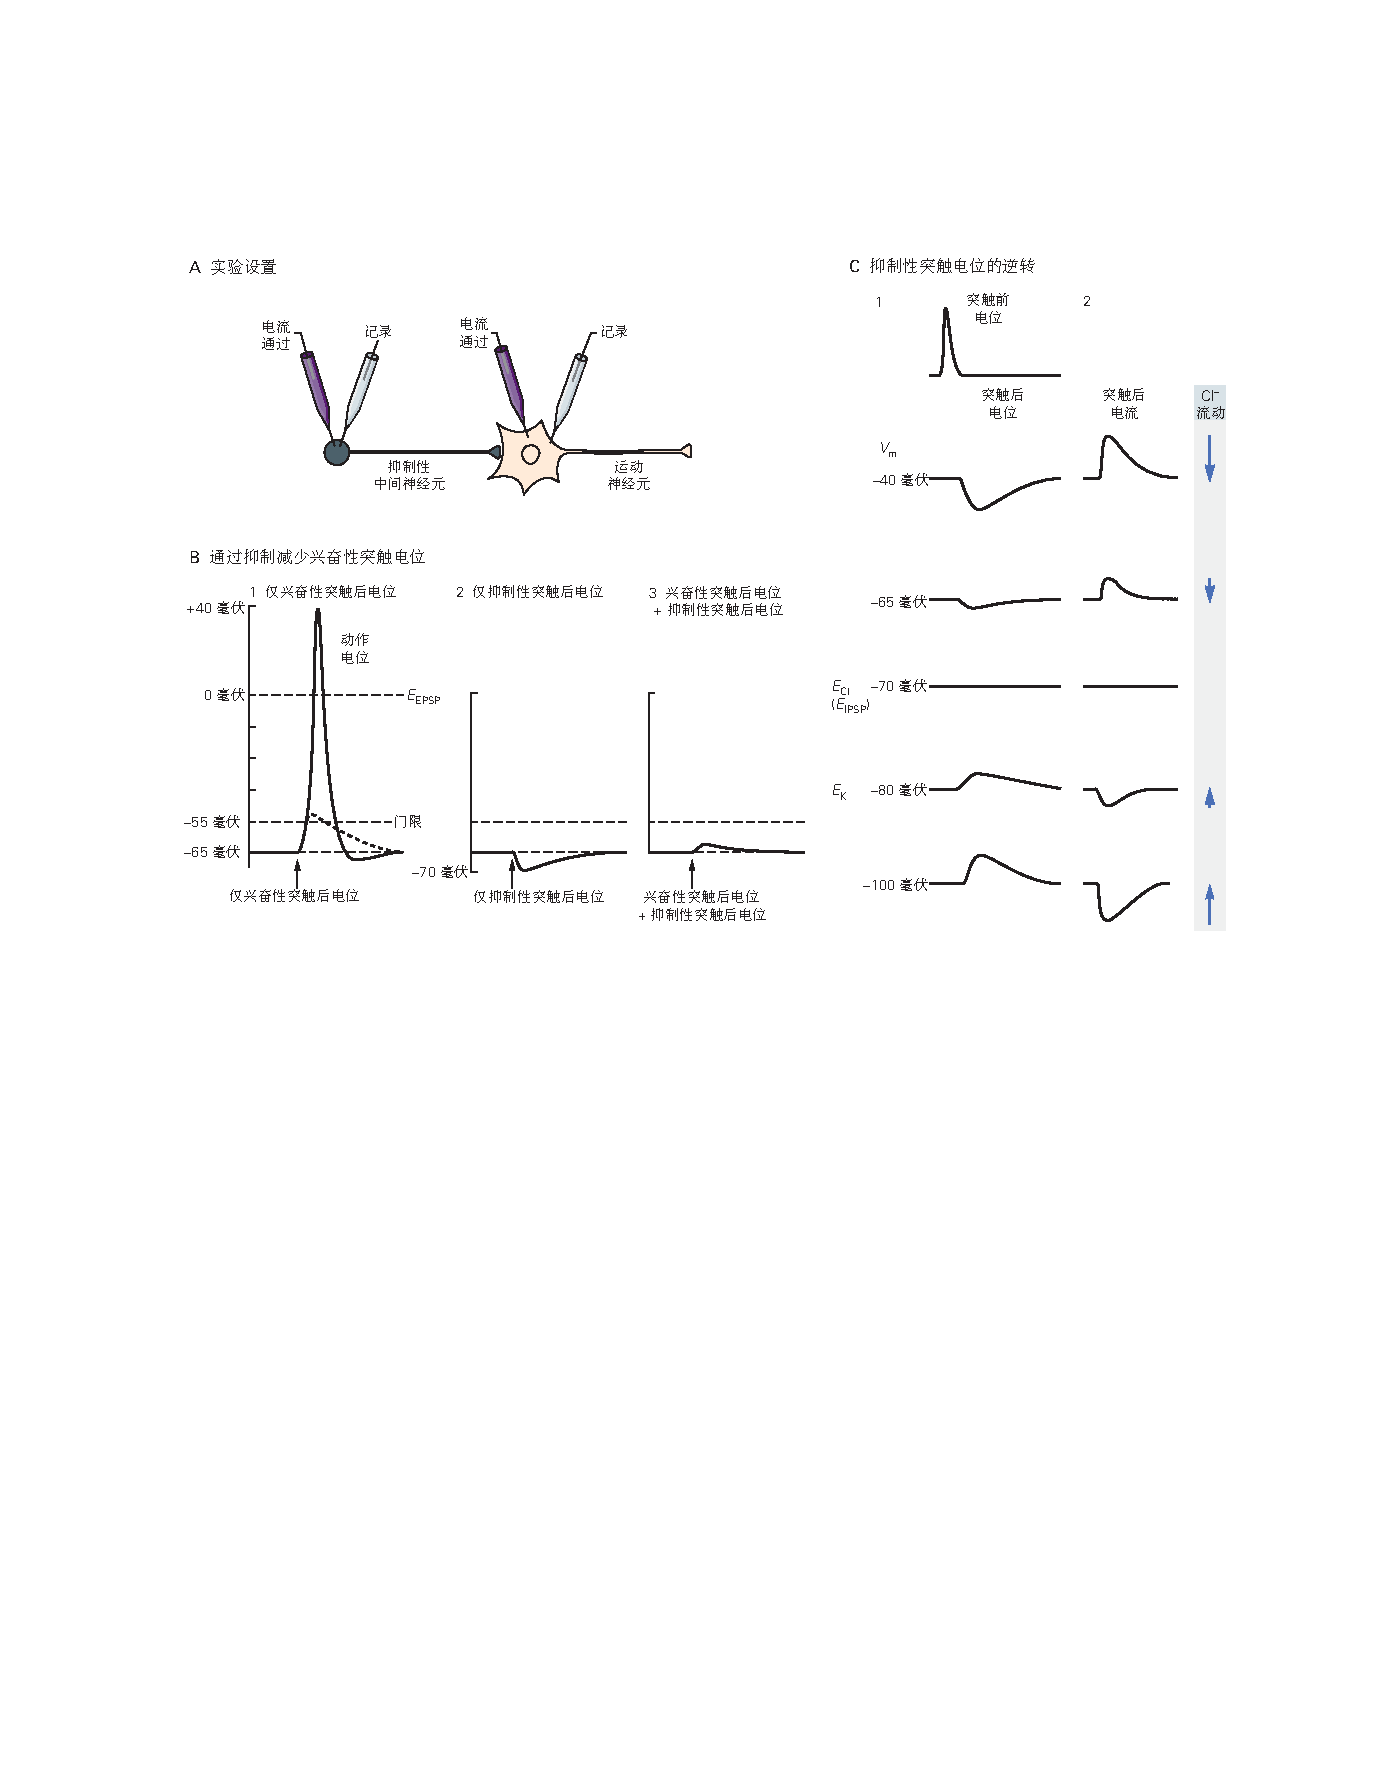
\includegraphics[width=0.95\linewidth]{chap13/fig_13_11}
	\caption{化学突触的抑制作用是由氯离子选择性离子通道的打开引起的。
		\textbf{A.} 在这个假设的实验中,两个电极放置在突触前中间神经元中,两个电极放置在突触后运动神经元中。
		突触前细胞中的电流通过电极用于产生动作电位;
		在突触后细胞中,它用于在突触前输入之前系统地改变膜电位。
		\textbf{B.} 抑制作用抵消兴奋作用。
		1. 单独出现的大\textit{兴奋性突触后电位}使膜去极化为 EEPSP,并超过产生动作电位的阈值。
		2. IPSP 单独将膜电位从阈值移向 ECl,即 Cl− 的平衡电位 (-70 毫伏)。
		3. 当抑制性和兴奋性突触电位同时出现时,\textit{兴奋性突触后电位}的有效性会降低,无法达到动作电位的阈值。
		\textbf{C.} IPSP 和抑制性突触电流在 ECl 处反转。
		1. 突触前尖峰在静息膜电位 (−65 毫伏) 处产生超极化 IPSP。
		由于 \ce{Cl-} 上的内向驱动力增加,当膜电位设置为 -40 毫伏时,IPSP 较大。
		当膜电位设置为 −70 毫伏时,IPSP 无效。
		IPSP 的这种逆转潜力发生在 ECl。 随着膜的进一步超极化,\textit{抑制性突触后电位}反转为去极化突触后电位(-80 和 -100 毫伏),因为膜电位对 ECl 为负。
		2. 电压钳下测得的抑制性突触后电流的反转电位。
		内向(负)电流在膜电位与反转电位相反(对应于 \ce{Cl-} 的流出)处流动,而向外(正)电流在膜电位与反转电位正相关(对应于 \ce{Cl-} 的流入)处流动。
		(向上箭头 = 流出;向下箭头 = 流入。)}
	\label{fig:13_11}
\end{figure}


当运动神经元膜保持在正常静息电位 (-65 毫伏) 时,当突触前中间神经元受到刺激时会产生一个小的超极化电位。
当运动神经元膜保持在-70 毫伏时,刺激中间神经元时不会记录到电位变化。
但在低于-70 毫伏的电位下,运动神经元在抑制性中间神经元受到刺激后会产生去极化反应。
这种 -70 毫伏的反转电位对应于脊髓运动神经元中的 \ce{Cl-} 平衡电位(\ce{Cl-} 的细胞外浓度远大于细胞内浓度)。
因此,在 -70 毫伏时,\ce{Cl-} 沿着其化学浓度梯度扩散到细胞中的趋势被反对 \ce{Cl-} 流入的电力(负膜电位)所平衡。
根据能斯特方程的预测,用非渗透性阴离子替代细胞外 \ce{Cl-} 会减小\textit{抑制性突触后电位}的大小,并将反转电位转变为更正的值。
因此,\textit{抑制性突触后电位}是由 \ce{Cl-} 电导的增加引起的。


已经使用膜片钳技术测量了通过单个\textit{$\gamma$-氨基丁酸}和甘氨酸受体通道的电流,单一电流。
两种递质都激活以全氮-无方式打开的 \ce{Cl-} 通道,类似于\textit{乙酰胆碱}和谷氨酸门控通道的打开。
\textit{$\gamma$-氨基丁酸}和甘氨酸对神经元放电的抑制作用取决于两个相关机制。
首先,在典型的神经元中,-65 毫伏的静息电位比 ECl (-70 毫伏) 略微更正。
在此静息电位下,驱动 Cl− 进入细胞的化学力略大于反对 Cl− 流入的电力——也就是说,Cl− (Vm − ECl) 上的电化学驱动力为正。
因此,根据 ICl = gCl (Vm − ECl) 的关系,Cl− 通道的打开会导致正电流。 因为电荷载体是带负电的 \ce{Cl-} 离子,正电流对应于 \ce{Cl-} 流入神经元,沿其电化学梯度下降。
这导致膜内部负电荷的净增加——膜变得超极化。


然而,一些中枢神经元的静息电位大约等于 ECl。 在此类细胞中,\ce{Cl-} 电导的增加不会改变膜电位 - 细胞不会变得超极化 - 因为 \ce{Cl-} 上的电化学驱动力几乎为零。
然而,此类细胞中 \ce{Cl-} 通道的打开仍然会抑制细胞响应几乎同时发生的\textit{兴奋性突触后电位}而激发动作电位。
这是因为兴奋性输入产生的去极化取决于所有类型开放通道的细胞的加权平均值 - 即兴奋性和抑制性突触电导的细胞以及静息电导 - 加权因子等于总 特定类型通道的电导(参见第~\ref{chap:chap12}~章,后记)。
因为 \ce{Cl-} 通道的细胞位于静息电位附近,打开这些通道有助于通过增加 \ce{Cl-} 细胞的加权因子在\textit{兴奋性突触后电位}期间将膜保持在其静息电位附近。


Cl− 通道的开放对\textit{兴奋性突触后电位}大小的影响也可以用欧姆定律来描述。
因此,\textit{兴奋性突触后电位}期间的去极化幅度 ΔVEPSP 由下式给出:


\begin{equation}\label{depolarization_amplitude}
	\delta V_{EPSP} = I_{EPSP} / g_1,
\end{equation}


其中 IEPSP 是兴奋性突触电流,gl 是膜中所有其他开放通道的电导,包括静息通道和传输门控 \ce{Cl-} 通道。 因为 \ce{Cl-} 通道的开放增加了静息电导,即使神经元更加渗漏,\textit{兴奋性突触后电位}期间的去极化减少。
突触抑制的这种后果称为短路或分流效应。


通过抵消突触兴奋,突触抑制可以对由于内在起搏器通道的存在而自发活跃的神经元中的动作电位放电施加强有力的控制。
这种称为抑制的雕刻作用的功能塑造了此类细胞的放电模式(图~\ref{fig:13_12})。 
事实上,抑制的这种塑造作用可能发生在所有神经元中,导致神经元脉冲的时间模式和神经回路同步的控制。


\begin{figure}[htbp]
	\centering
	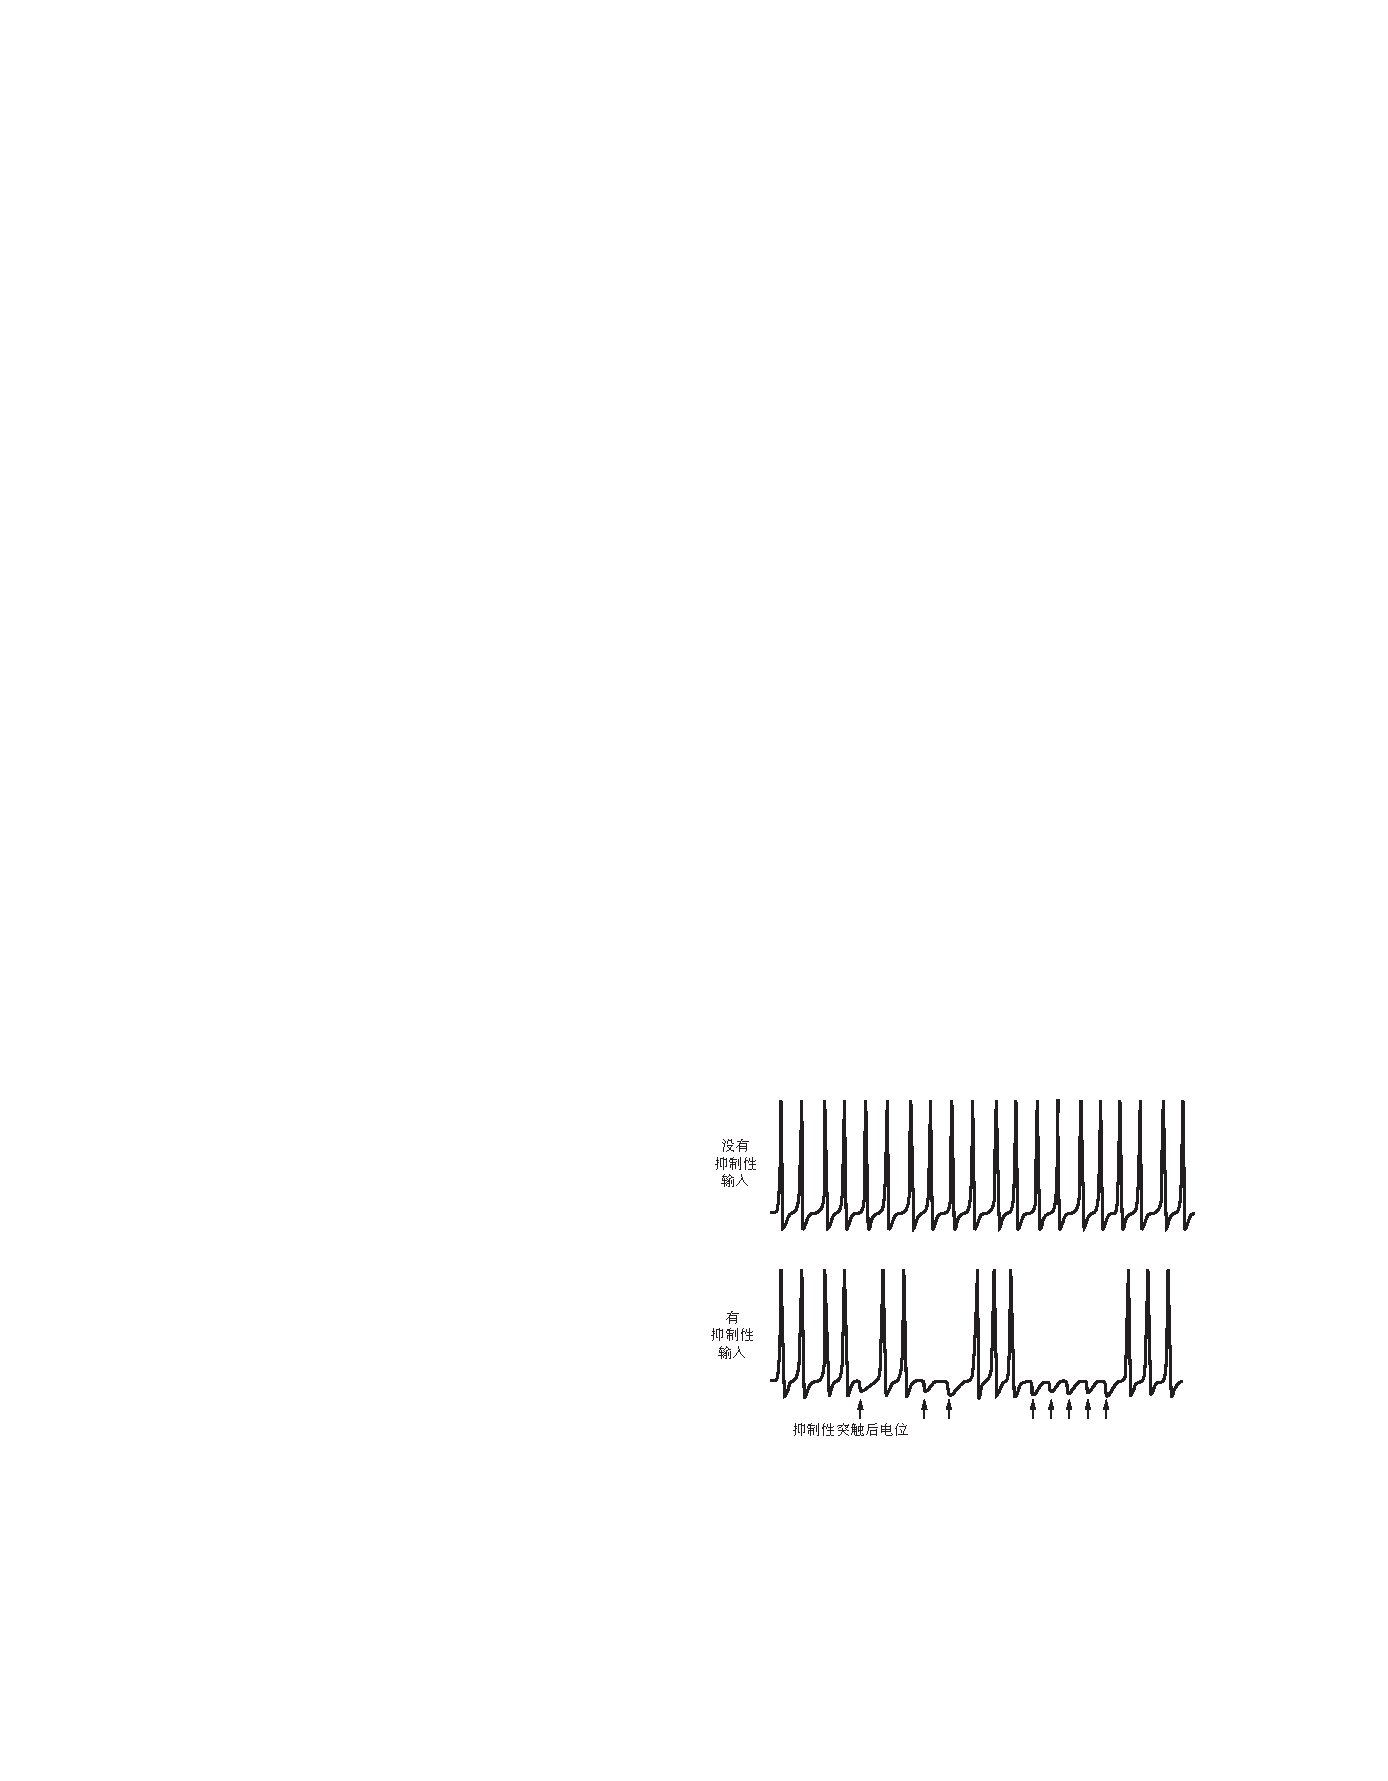
\includegraphics[width=0.5\linewidth]{chap13/fig_13_12}
	\caption{抑制可以塑造自发活跃神经元的放电模式。 在没有抑制性输入的情况下,神经元会以固定的时间间隔连续发射。 通过抑制性输入(箭头),一些动作电位被抑制,导致独特的冲动模式。}
	\label{fig:13_12}
\end{figure}


突触电导的不同生物物理特性可以理解为突触后神经元执行的不同数学运算。
因此,使细胞超极化的抑制性输入对兴奋性输入进行减法,而电导增加的分流效应进行除法。
添加兴奋性输入(或移除非分流抑制性输入)会导致求和。
最后,兴奋性输入与去除抑制性分流的组合产生乘法。
然而,这些算术效应通常是混合的,并且随着神经元膜电位不断变化而随时间变化,导致通过\textit{$\gamma$氨基丁酸A}受体通道对 Cl− 的驱动力发生变化。


在一些细胞中,例如那些具有代谢型 GABAB 受体的细胞,抑制是由 \ce{K+} 通道的开放引起的。
因为神经元的 \ce{K+} 平衡电位 (EK = −80 毫伏) 总是对静息电位负,所以打开 \ce{K+} 通道比打开 \ce{Cl-} 通道(假设具有相似大小的突触电导)更能抑制细胞,产生更多“ 减法”抑制。
与 \textit{$\gamma$氨基丁酸A} 响应相比,GABAB 响应开启得更慢并且持续时间更长。


矛盾的是,在某些情况下,脑细胞中 \textit{$\gamma$氨基丁酸A} 受体的激活会引起兴奋。
这是因为在强烈刺激后 \ce{Cl-} 的流入可能非常大,以至于细胞内 \ce{Cl-} 浓度显着增加。
它甚至可能翻倍。
结果,\ce{Cl-} 平衡电位可能变得比静息电位更正。
在这些条件下,\ce{Cl-} 通道的开放导致 \ce{Cl-} 流出和神经元去极化。
这种去极化 \ce{Cl-} 反应通常发生在新生动物的许多神经元中,其中细胞内 \ce{Cl-} 浓度即使在静止时也往往很高。
这是因为负责维持低细胞内 \ce{Cl-} 的 \ce{K+}-\ce{Cl-} 协同转运蛋白在早期发育期间以低水平表达(第 ~\ref{chap:chap9}~章)。
去极化 \ce{Cl-} 反应也可能发生在更成熟神经元的远端树突中,也可能发生在它们的轴突初始段。
成人中的这种兴奋性 \textit{$\gamma$氨基丁酸A} 受体作用可能有助于癫痫放电,其中观察到大量、同步和去极化的 GABA 反应。



\section{中枢神经系统中的一些突触动作依赖于其他类型的离子型受体}

大脑中少数快速兴奋性突触动作是由作用于\textit{5-羟基色氨酸}3 类离子型受体通道的神经递质\textit{5-羟基色氨酸}介导的。
这些五聚体受体由具有四个跨膜区段的亚基组成,在结构上类似于烟碱\textit{乙酰胆碱}受体。
与\textit{乙酰胆碱}受体通道一样,\textit{5-羟基色氨酸}3 受体通道可渗透单价阳离子,并具有接近 0 毫伏的逆转电位。


三磷酸腺苷 (ATP) 的离子型受体在其他选定的突触中发挥兴奋作用,并构成第三个传递离子通道家族。
这些所谓的嘌呤能受体(以腺苷中的嘌呤环命名)出现在由自主神经节的交感神经元以及某些中枢和外周神经元支配的平滑肌细胞上。
在这些突触处,ATP 激活一个离子通道,该通道可渗透单价阳离子和 \ce{Ca^2+},反转电位接近 0 毫伏。
已经鉴定了编码该离子型 ATP 受体(称为 P2X 受体)家族的几个基因。
这些 ATP 受体的氨基酸序列和亚基结构不同于其他两个配体门控通道家族。
P2X 受体的 X 射线晶体结构显示它具有极其简单的组织,其中三个亚基(每个仅包含两个跨膜片段)围绕着一个中央孔(图~\ref{fig:13_4}C)。



\section{神经元将兴奋性和抑制性突触动作整合为单一输出}

中枢神经系统中的每个神经元不断受到来自许多其他神经元的一系列突触输入的轰击。
例如,一个运动神经元可能是多达 10,000 个不同突触前末梢的目标。
有些是兴奋性的,有些是抑制性的;
有些强,有些弱。
一些输入在其顶端树突的尖端接触运动细胞,其他的在近端树突上,一些在树突轴上,其他的在体细胞上。
不同的输入可以相互加强或抵消。
给定的神经元如何将这些信号整合成一致的输出?


正如我们之前看到的,单个突触前神经元产生的突触电位通常不足以将突触后细胞去极化到动作电位的阈值。
大多数拉伸敏感传入神经元在运动神经元中产生的\textit{兴奋性突触后电位}振幅仅为 0.2 至 0.4 毫伏。
如果单个运动神经元中产生的\textit{兴奋性突触后电位}线性求和,则至少 25 个传入神经元必须一起发射并释放发射器以使触发区去极化达到阈值所需的 10 毫伏。
但在突触后细胞接收兴奋性输入的同时,它也可能接收抑制性输入,通过减法或分流效应阻止动作电位的发射。


因此,任何单个兴奋性或抑制性突触的输入的净效应将取决于几个因素:
突触的位置、大小和形状;
其他协同或拮抗突触的接近度和相对强度;
和细胞的静息电位。 
此外,所有这一切都非常依赖于兴奋性和抑制性输入的时间。
输入在突触后神经元中通过称为神经元整合的过程进行协调。
这个细胞过程反映了整个神经系统所面临的任务。
在任何给定时刻,细胞都有两种选择:激发或不激发动作电位。
\textit{查尔斯·谢林顿}将大脑在相互竞争的选项之间进行选择的能力描述为神经系统的综合作用。
他认为这种决策是大脑最基本的运作(见第 ~\ref{chap:chap56}~章)。



\subsection{突触输入整合在轴突初始段}

在大多数神经元中,启动动作电位输出的决定是在一个部位做出的:轴突起始段。
此处,细胞膜的动作电位生成阈值低于细胞体或树突,因为它具有更高密度的电压依赖性 \ce{Na+} 通道(图 ~\ref{fig:13_13})。
随着膜去极化的每次增加,更多的 \ce{Na+} 通道打开,在轴突初始段提供比细胞其他地方更高的内向电流密度(每单位膜面积)。


\begin{figure}[htbp]
	\centering
	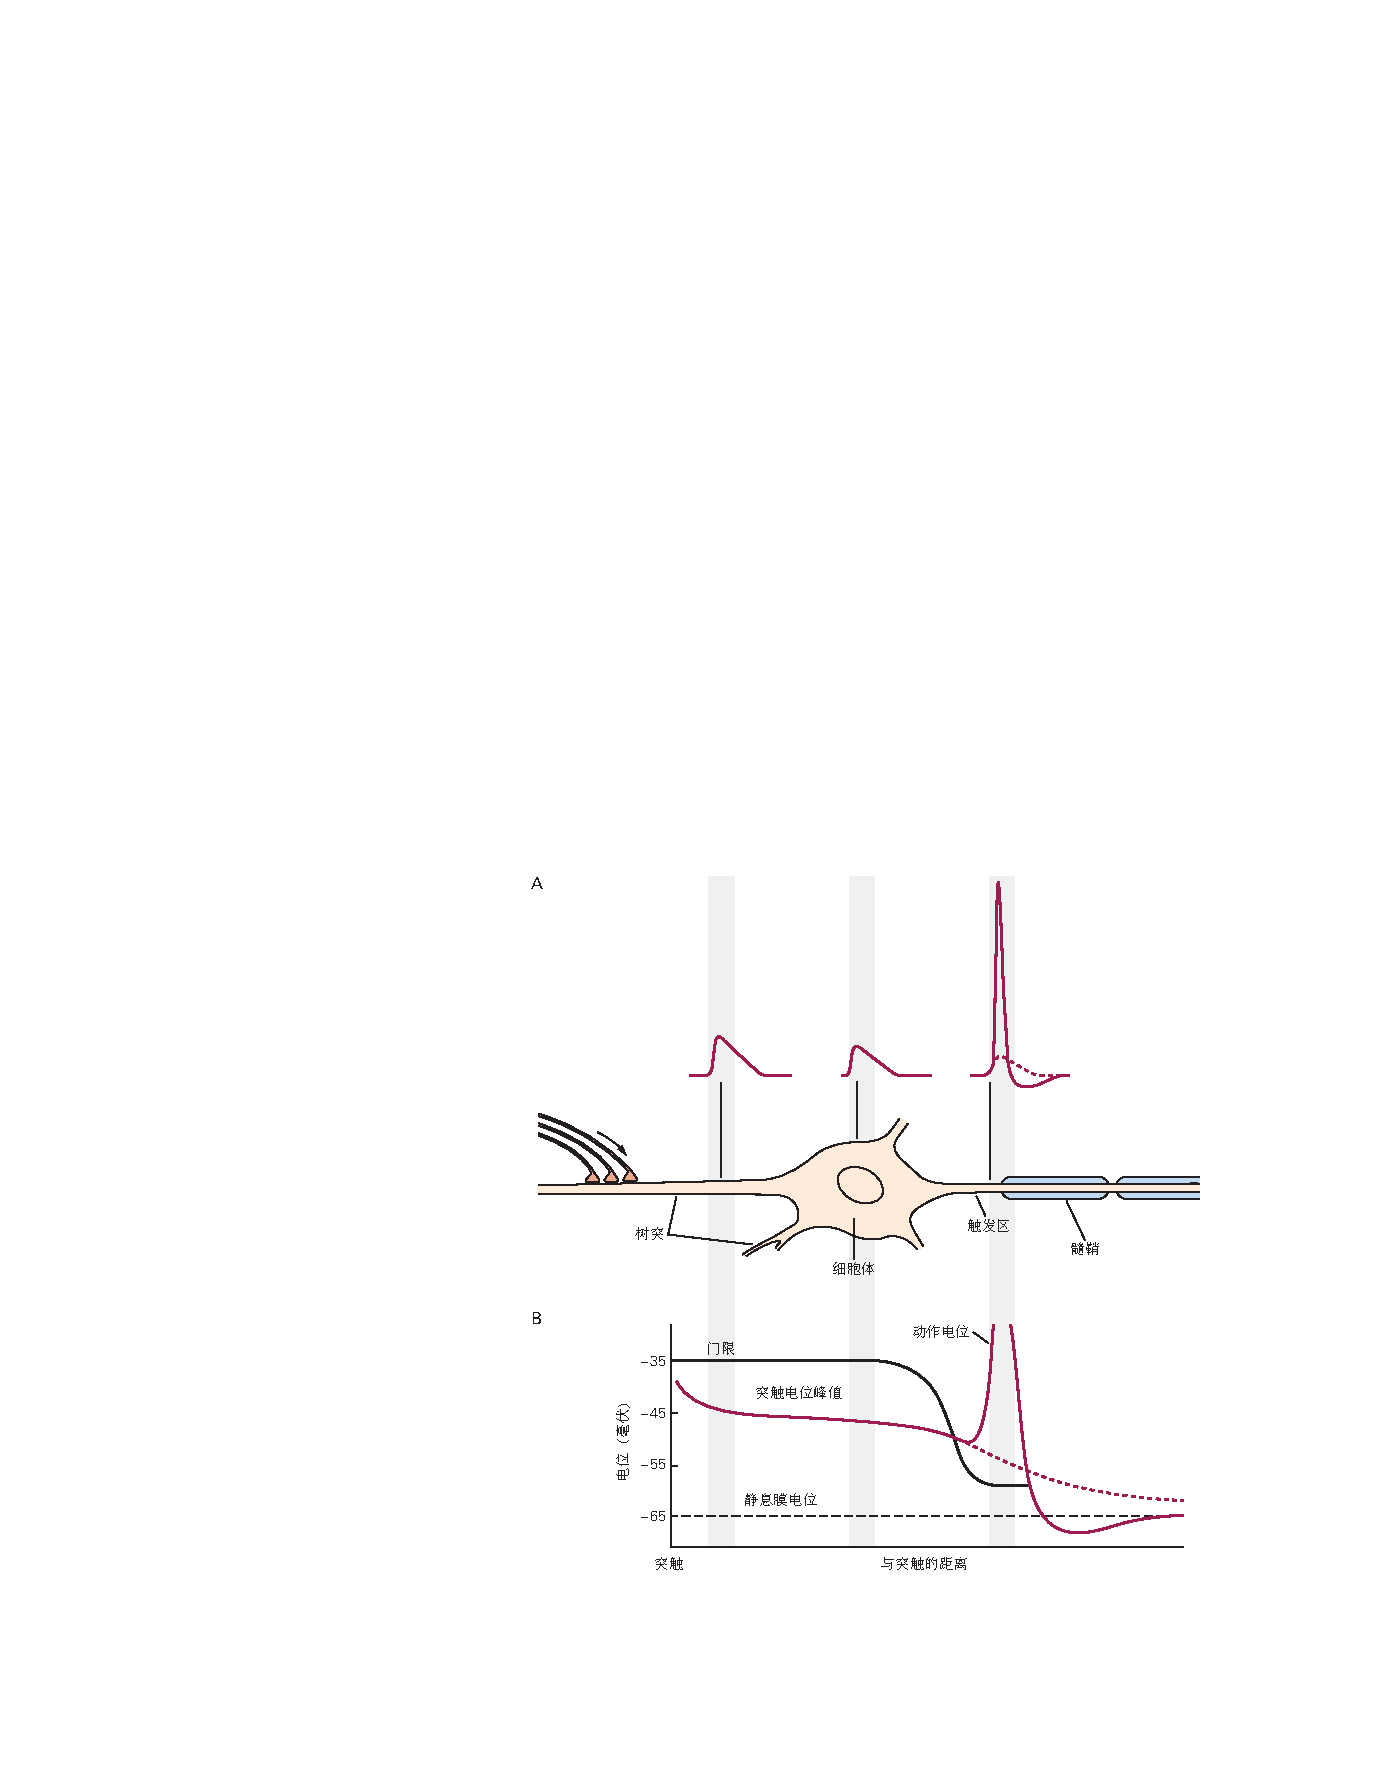
\includegraphics[width=0.7\linewidth]{chap13/fig_13_13}
	\caption{树突中产生的突触电位可以在轴突起始段产生动作电位\cite{eckert1988propagation}。
		\textbf{A.} 起源于树突的兴奋性突触电位随着距离的增加而降低,因为它被动地传播到躯体。
		然而,动作电位可以在触发区(轴突起始段)启动,因为该区域的 \ce{Na+} 通道密度高,因此动作电位的阈值较低。
		\textbf{B.} 神经元不同部位动作电位启动阈值的比较(对应于图 A)。
		当突触电位的幅度超过阈值时,就会产生动作电位。
		如果在轴突初始段没有产生动作电位,则虚线显示突触电位的衰减。}
	\label{fig:13_13}
\end{figure}


在初始段,达到动作电位阈值 (-55 毫伏) 所需的去极化增量仅比静息水平 -65 毫伏高 10 毫伏。
相反,细胞体的膜必须在达到其阈值 (-35 毫伏) 之前去极化 30 毫伏。
因此,突触激发首先在初始段释放膜区域,也称为触发区。
然后在该位点产生的动作电位使细胞体膜去极化至阈值,同时沿轴突传播。


因为神经元整合涉及传播到触发区的突触电位的总和,所以它受到神经元的两个被动膜特性的严重影响(第  ~\ref{chap:chap9}~章)。
首先,膜时间常数有助于确定突触电位响应 EPSC 的时间进程,从而控制时间总和,即突触后细胞中连续突触电位相加的过程。
具有大膜时间常数的神经元比具有较短时间常数的神经元具有更大的时间总和能力(图~\ref{fig:13_14} A)。
结果,时间常数越长,两个连续输入相加使细胞膜达到动作电位阈值的可能性就越大。


\begin{figure}[htbp]
	\centering
	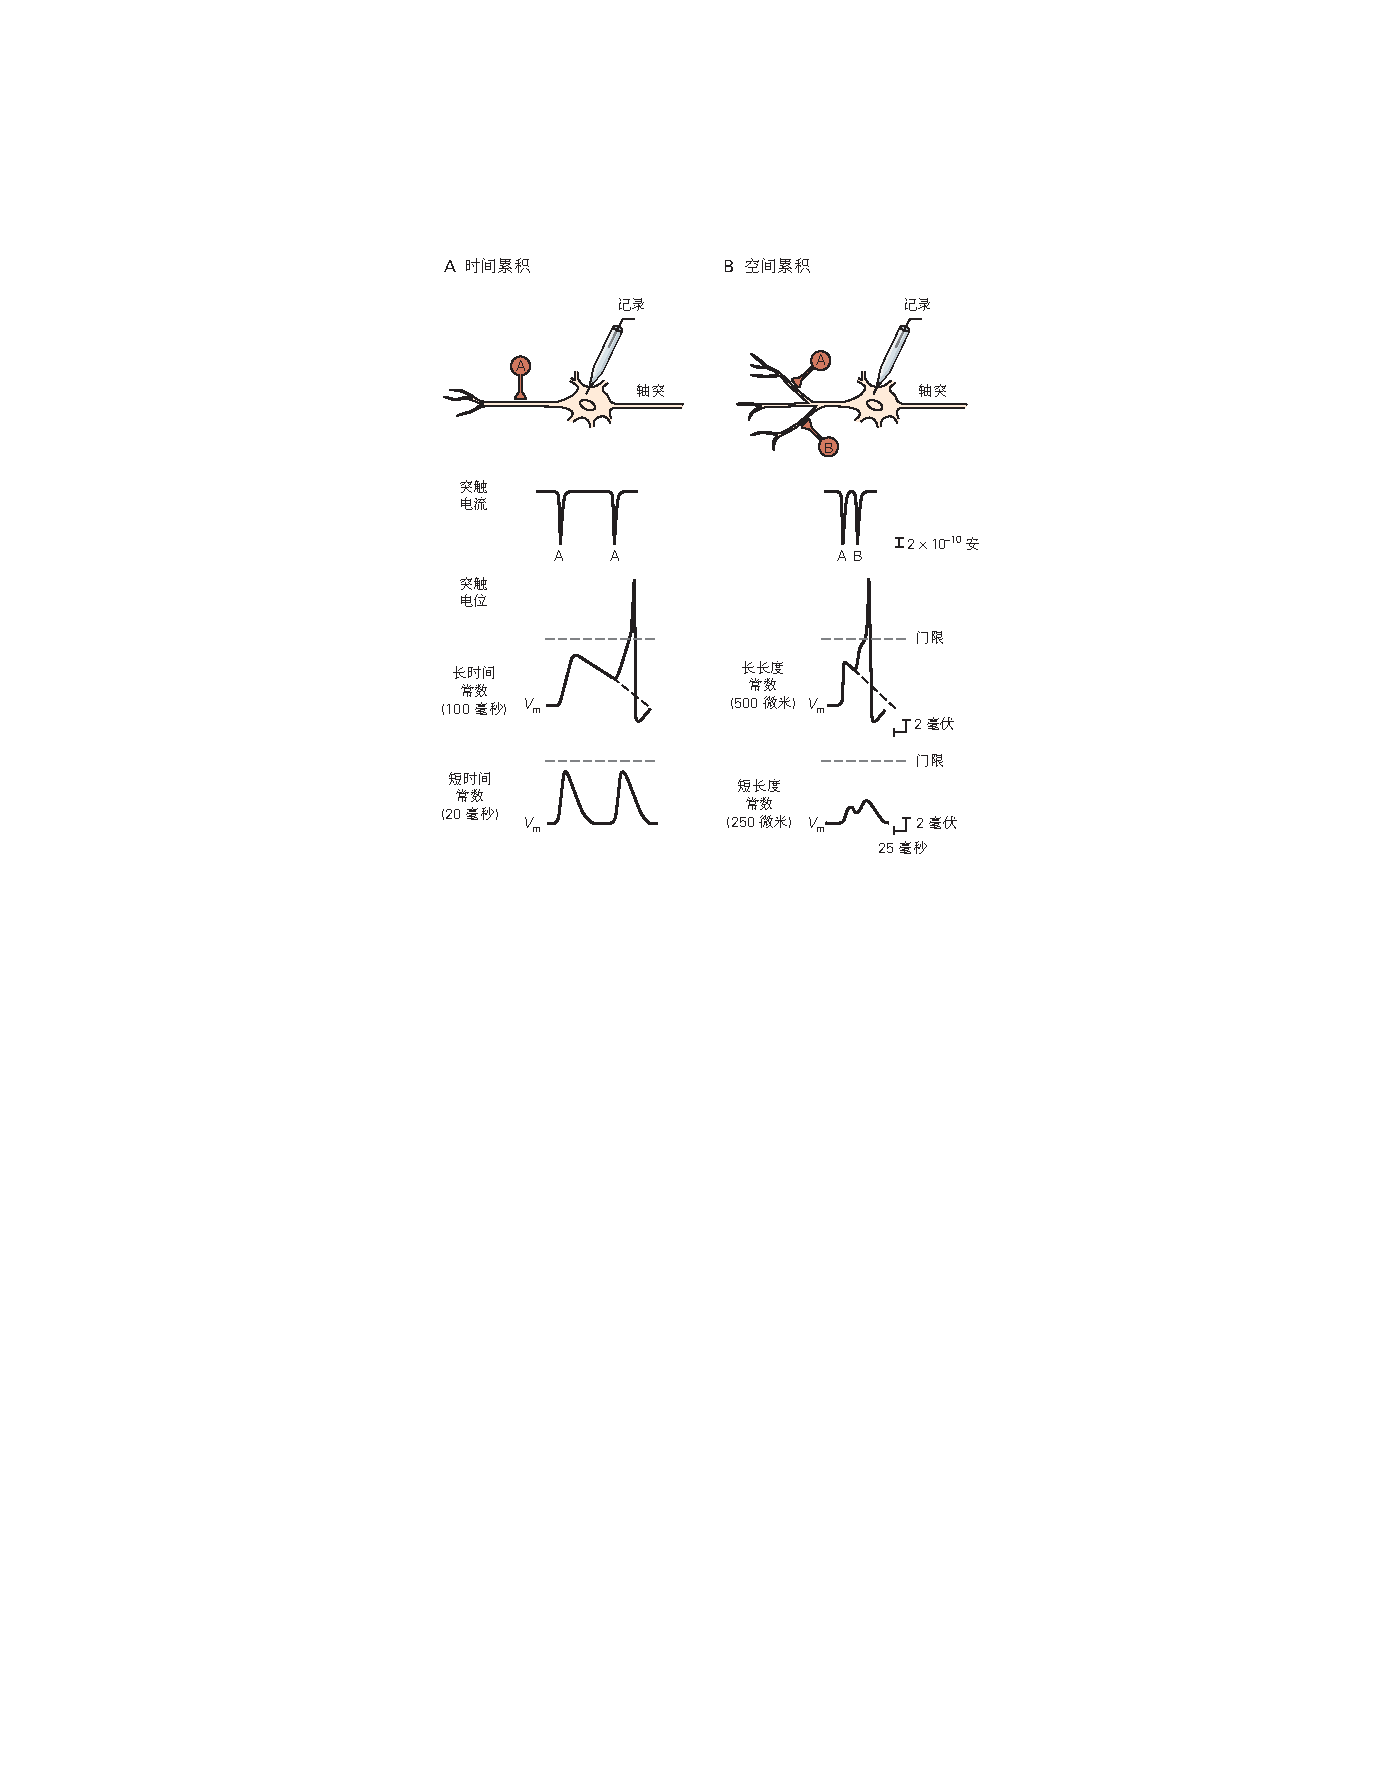
\includegraphics[width=0.6\linewidth]{chap13/fig_13_14}
	\caption{中枢神经元能够通过突触电位的时间和空间总和来整合各种突触输入。
		\textbf{A.} 时间总和。
		突触后细胞的时间常数(参见图~\ref{fig:9_10})影响由单个突触前神经元(细胞 A)产生的连续 \textit{兴奋性突触后电位} 引起的去极化幅度。
		在这里,两个 \textit{兴奋性突触后电位} 的突触前神经元产生的突触电流几乎相同。
		在具有较长时间常数的电池中,第一个 \textit{兴奋性突触后电位} 不会在第二个 \textit{兴奋性突触后电位} 被触发时完全衰减。
		在那种情况下,两种电位的去极化效应是相加的,使膜电位高于阈值并触发动作电位。
		在具有短时间常数的细胞中,第一个 \textit{兴奋性突触后电位} 在第二个 \textit{兴奋性突触后电位} 被触发之前衰减到静息电位,在这种情况下,单独的第二个\textit{兴奋性突触后电位}不会引起足够的去极化来触发动作电位。
		\textbf{B.} 空间求和。
		突触后细胞的长度常数(参见图~\ref{fig:9_11}B)影响两个突触前神经元(细胞 A 和 B)产生的两个兴奋性突触后电位的振幅。
		出于说明目的,两个突触与突触后细胞触发区的距离相同 (500 微米),并且每个突触接触产生的电流相同。
		如果突触输入位点与突触后细胞触发区的距离只有一个长度常数(即突触后细胞的长常数为500微米),则两个突触前神经元各自产生的突触电位 当它们到达触发区时,将减小到原始振幅的 37\%。
		两个电位的总和导致足够的去极化超过阈值,触发动作电位。
		如果突触和触发区之间的距离等于两个长度常数(即突触后细胞的短长度常数为 250 微米),则每个突触电位将小于其初始振幅的 15\%,并且求和不会 足以触发动作电位。}
	\label{fig:13_14}
\end{figure}


其次,细胞的长度常数决定了\textit{兴奋性突触后电位}减少的程度,因为它从突触沿着树突的长度被动扩散到细胞体和轴突初始段(触发区)。
在具有较长长度常数的单元格中,信号以最小的衰减传播到触发区域;
在具有短长度常数的细胞中,信号随距离迅速衰减。
由于一个突触产生的去极化几乎永远不足以在触发区触发动作电位,因此必须将作用于突触后神经元不同部位的许多突触前神经元的输入加在一起。
这个过程称为空间求和。
与长度常数较短的神经元相比,长度常数较大的神经元更有可能被来自不同部位的输入带到阈值(图~\ref{fig:13_14}B)。



\subsection{\textit{$\gamma$-氨基丁酸}能神经元的亚类靶向其突触后靶神经元的不同区域以产生具有不同功能的抑制作用}

与相对较少类型的谷氨酸能锥体神经元相比,哺乳动物中枢神经系统具有种类繁多的\textit{$\gamma$-氨基丁酸}能抑制性中间神经元,它们在发育起源、分子组成、形态和连通性方面各不相同(图~\ref{fig:13_15})。
仅在海马体的一个分区中,就已鉴定出多达 20 种不同的\textit{$\gamma$-氨基丁酸}能神经元亚型。
不同类型的\textit{$\gamma$-氨基丁酸能}中间神经元与其邻近的兴奋性和抑制性神经元形成广泛的突触连接。
因此,即使所有神经元中只有 20\% 是抑制性的,但在大多数大脑区域中,抑制和兴奋的总体水平往往接近平衡。
这导致调整神经回路以仅响应最显着的兴奋信息。
虽然中间神经元的多样性很难理解,但很明显,不同类型的中间神经元选择性地针对其突触后神经元的不同区域。


\begin{figure}[htbp]
	\centering
	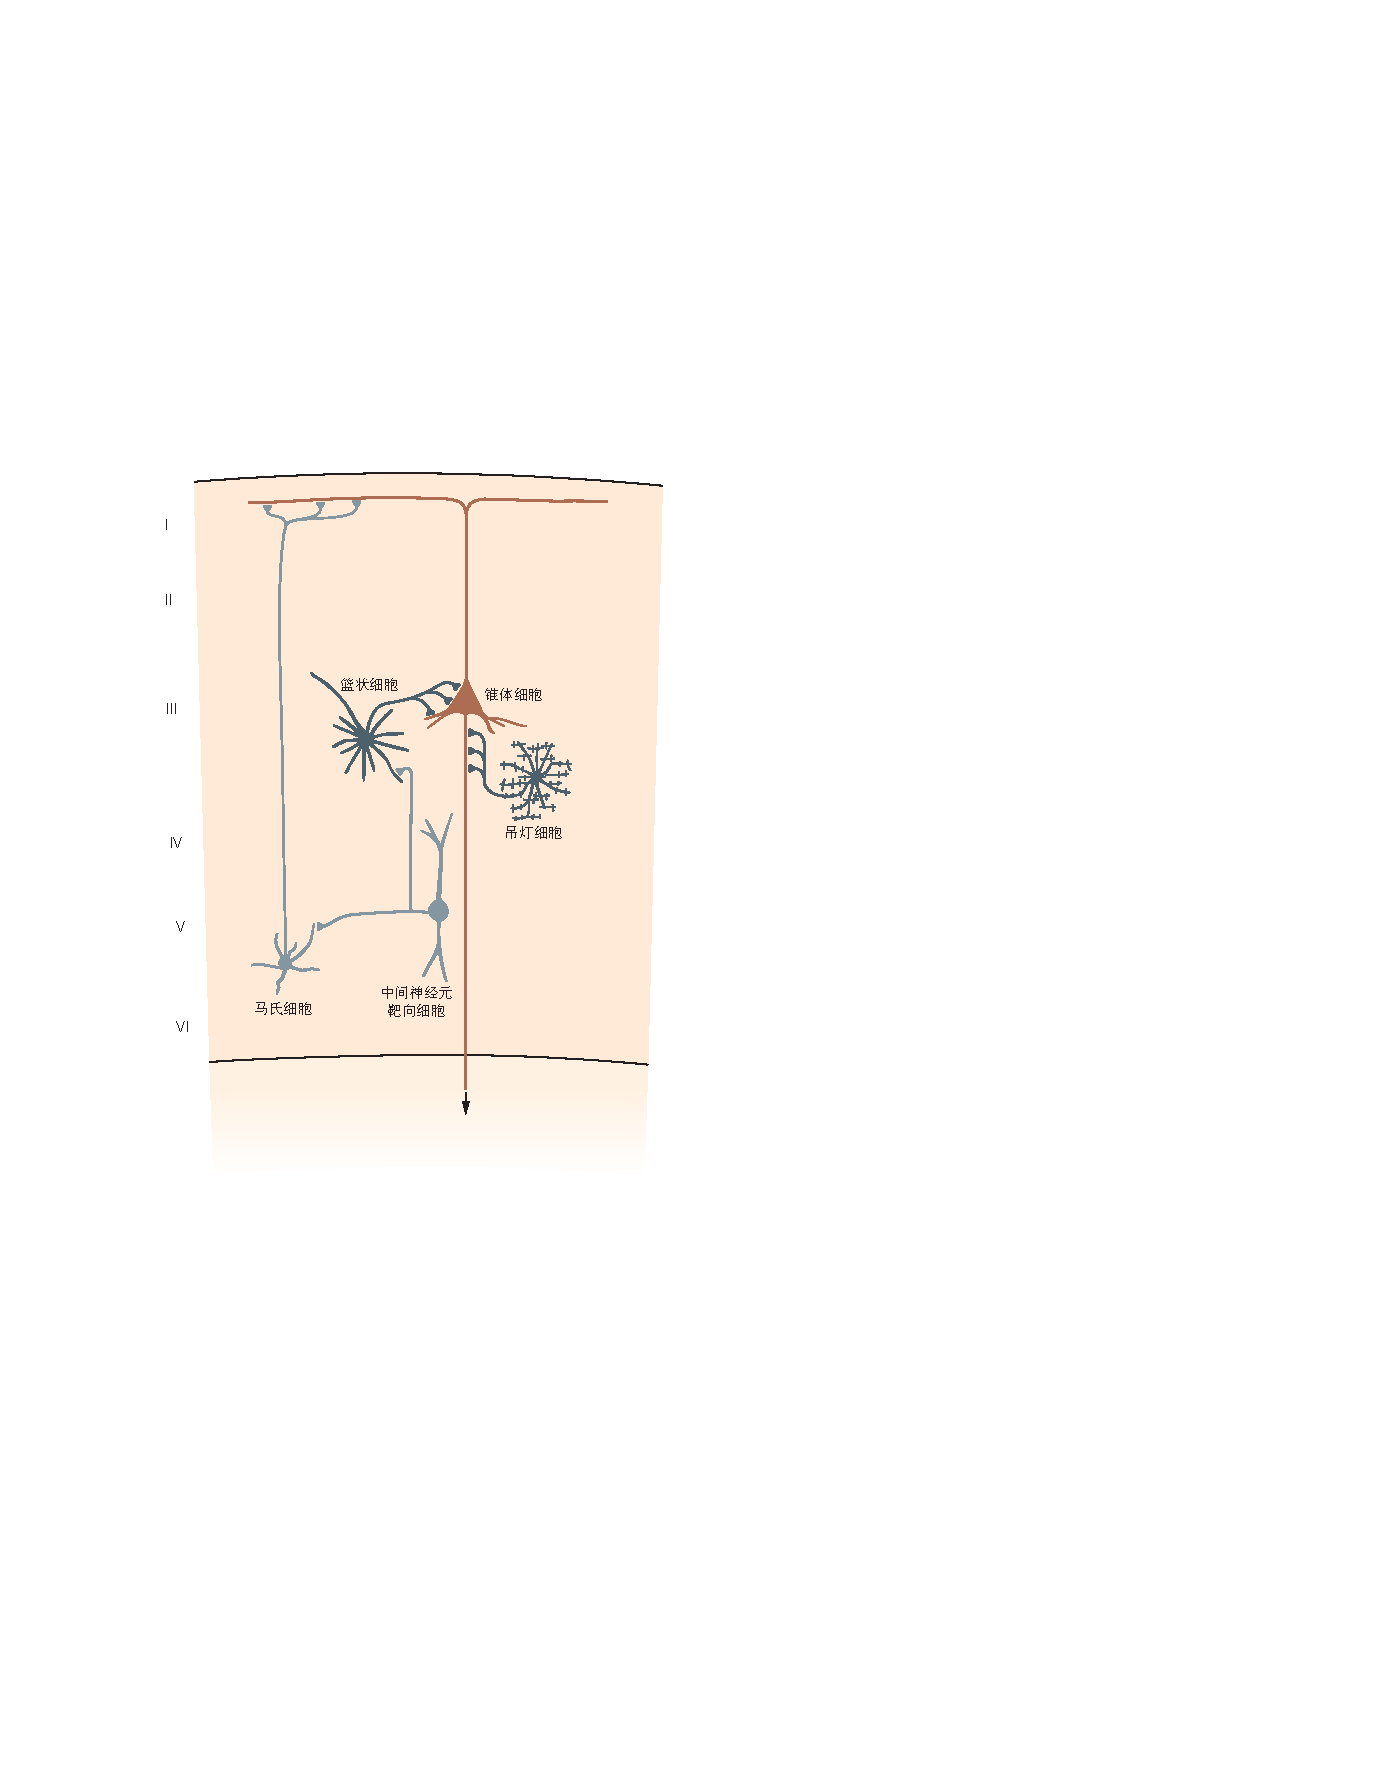
\includegraphics[width=0.5\linewidth]{chap13/fig_13_15}
	\caption{不同的\textit{$\gamma$-氨基丁酸}能抑制神经元针对突触后细胞的不同区域。
		可以通过它们的形态、不同分子标记的表达以及它们首选的突触后神经元靶向位点来区分各种各样的中间神经元。
		篮状细胞发送它们的轴突在细胞体和突触后神经元的近端树突上形成突触。
		篮状细胞的树突显示为从体细胞辐射的短线。
		轴突细胞,也称为枝形吊灯细胞,发送它们的轴突以沿着其目标的轴突初始段形成突触簇。
		篮子细胞和枝形吊灯细胞都表达钙结合蛋白小清蛋白。
		树突靶向细胞,也称为 Martinotti 细胞,发送它们的轴突在锥体细胞的远端树突上形成突触。
		这些细胞还释放神经肽生长抑素。
		其他类别的\textit{$\gamma$-氨基丁酸}能神经元选择性地与其他抑制性中间神经元形成突触。
		除了\textit{$\gamma$-氨基丁酸}之外,这些中间神经元靶向抑制性神经元通常还会释放神经肽 Y。}
	\label{fig:13_15}
\end{figure}


这种选择性靶向很重要,因为与兴奋性突触相关的抑制性输入的位置对于确定抑制的有效性至关重要(图 ~\ref{fig:13_16})。
当在细胞体或轴突触发区附近启动抑制时,响应兴奋性输入的动作电位输出抑制更有效。
当树突向轴突移动时,由树突的兴奋电流产生的去极化必须沿着细胞体膜传递。
细胞体或轴突起始段的抑制作用会打开 \ce{Cl-} 通道,从而增加 \ce{Cl-} 电导并减少(通过分流)由扩散的兴奋电流产生的大部分去极化。
此外,当抑制输入针对细胞体而不是树突时,细胞体响应\textit{抑制性突触后电位}的超极化大小最大,这是由于树突的电缆特性导致树突 IPSP 衰减。


\begin{figure}[htbp]
	\centering
	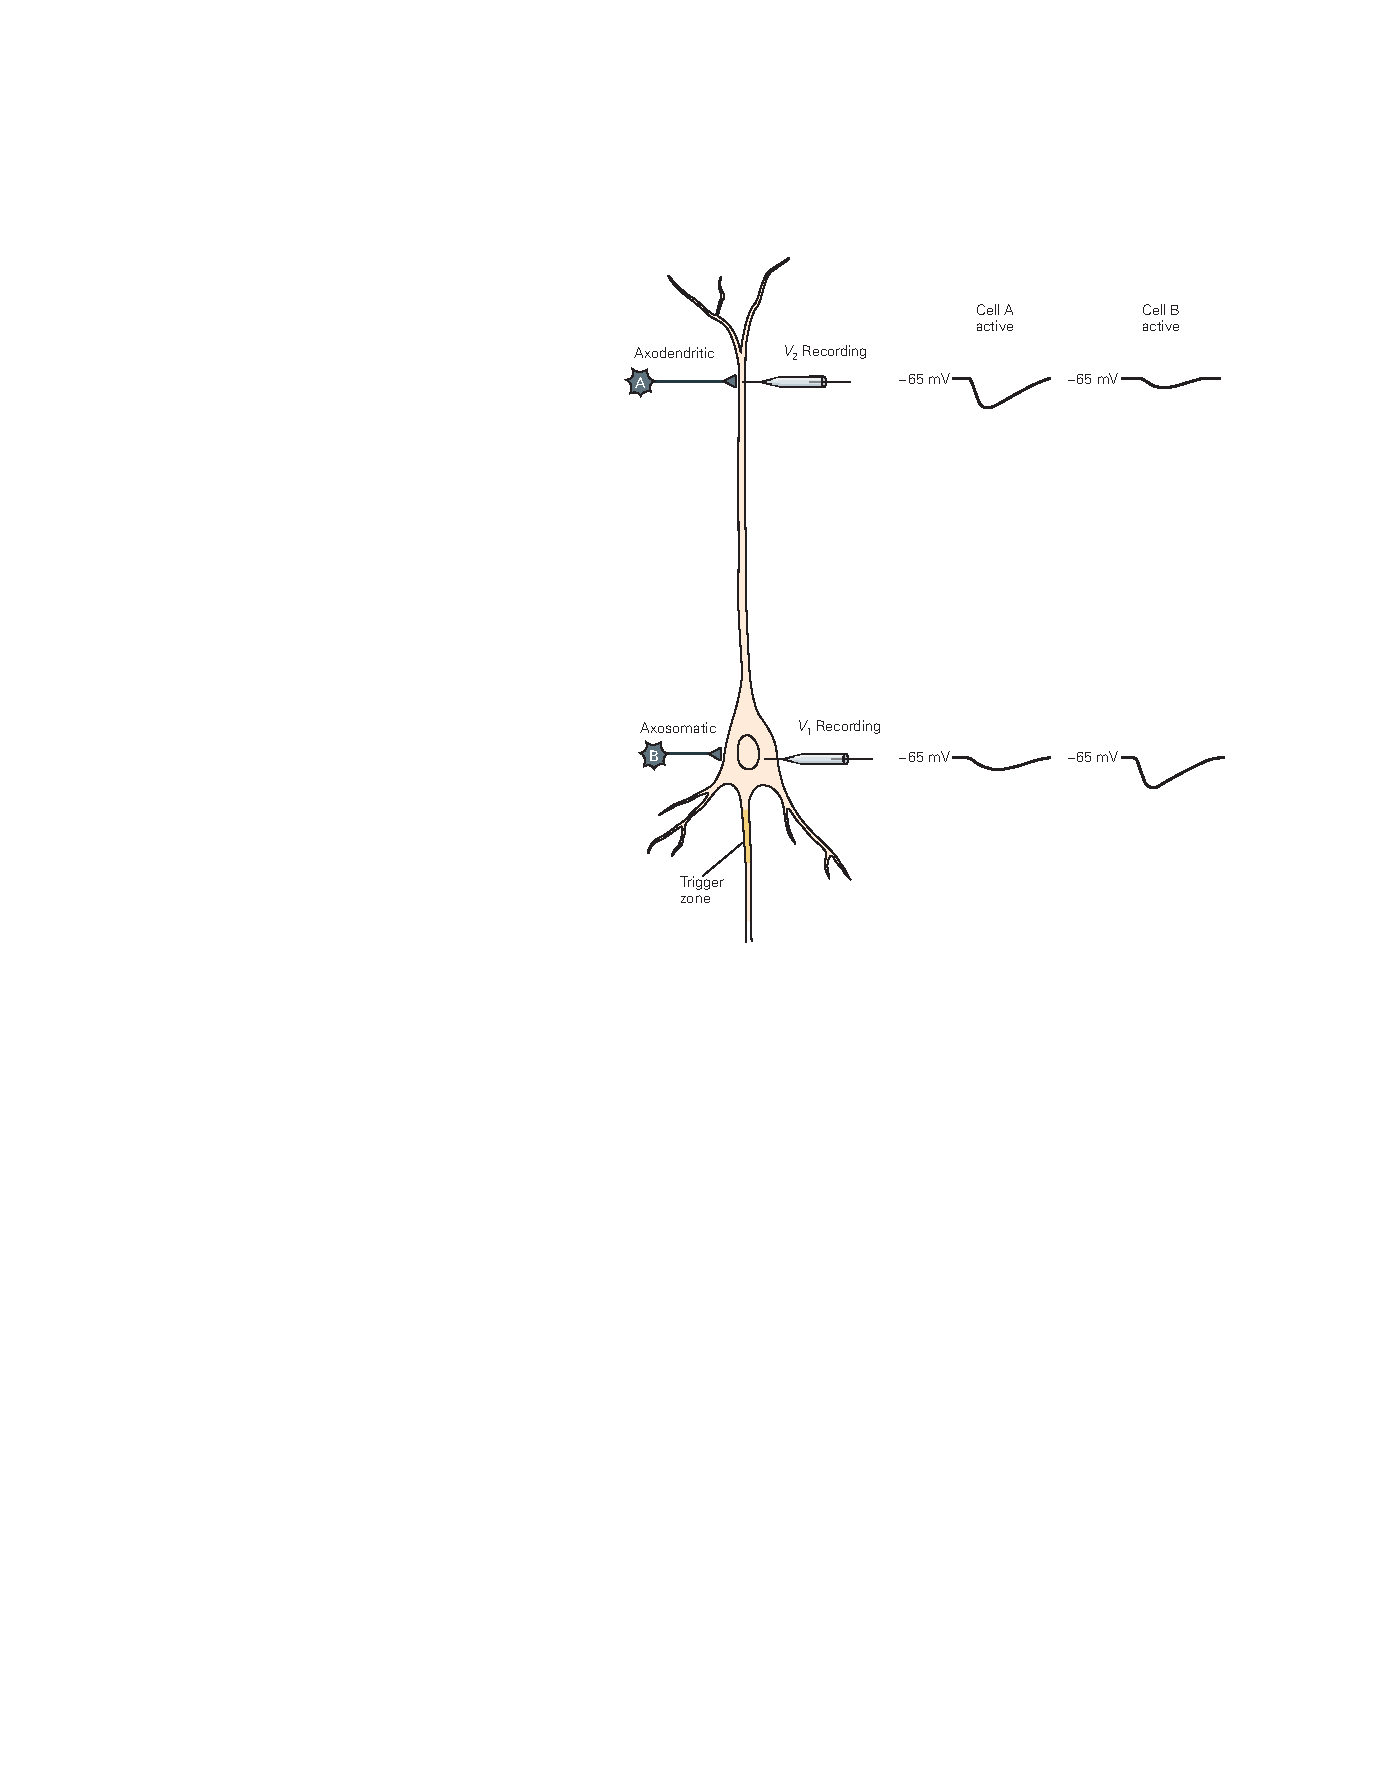
\includegraphics[width=0.6\linewidth]{chap13/fig_13_16}
	\caption{突触后神经元中抑制电流的作用取决于电流从突触到细胞触发区的距离。 在这个假设的实验中,通过从突触后细胞的细胞体 (V1) 和树突 (V2) 记录来比较抑制性轴体突触和轴突突触的输入。 刺激细胞 B(轴体突触)在细胞体中产生一个大的 IPSP。 IPSP 在树突上传播时衰减,在树突记录的位置仅产生小的超极化。 刺激细胞 A 激活轴突突触,在树突中产生一个大的局部 IPSP,但在细胞体中只产生一个小的 IPSP,因为突触电位在沿着树突传播时会衰减。 因此,轴体 IPSP 在抑制突触后细胞动作电位放电方面比轴突\textit{抑制性突触后电位}更有效,而轴突\textit{抑制性突触后电位}在防止局部树突去极化方面更有效。}
	\label{fig:13_16}
\end{figure}


两类抑制性神经元,篮子细胞和枝形吊灯细胞,分别通过特异性靶向体细胞和轴突起始段来对神经元输出施加强大的控制(图~\ref{fig:13_15})。
篮状细胞通常表达钙结合蛋白小白蛋白,是大脑中最常见的抑制性神经元类型。
也表达小白蛋白的枝形吊灯细胞具有轴突乔木,其具有分支模式和突触末端集群,类似于枝形吊灯的众多蜡烛。
在某些情况下,枝形吊灯细胞可能会反常地增强神经元放电,因为某些轴突中的 \ce{Cl-} 反转电位可能与动作电位放电的阈值正相关。


第三类中间神经元,即 Martinotti 细胞,专门针对远端树突和棘。
除了\textit{$\gamma$-氨基丁酸}之外,这些常见的中间神经元还释放神经肽生长抑素。
树突远端部分的抑制作用可减少附近兴奋性输入产生的局部去极化,对其他树突分支上产生的\textit{兴奋性突触后电位}影响较小。
生长抑素阳性的中间神经元响应兴奋性输入而缓慢激活,并生成随着重复激活(突触促进)而增加大小的\textit{抑制性突触后电位}。 
相比之下,表达小白蛋白的中间神经元会快速放电并生成\textit{抑制性突触后电位},\textit{抑制性突触后电位}的大小会随着重复激活(突触抑制)而减小。
这些特性允许生长抑素和小清蛋白中间神经元分别控制神经信号后期和早期阶段通过神经回路的传播。


第四种主要类型的抑制性中间神经元表达神经肽血管活性肠肽 (VIP)。
这些中间神经元选择性地靶向其他中间神经元,从而降低神经回路中的抑制水平,从而增强整体兴奋,这一过程称为去抑制。



\subsection{树突是可以放大突触输入的电激发结构}

信号在树突中的传播最初被认为是纯粹被动的。
然而,1950 年代神经元细胞体和 1970 年代开始的树突的细胞内记录表明,树突可以产生动作电位。
事实上,我们现在知道,除了配体门控通道和静息通道外,大多数神经元的树突还包含电压门控 \ce{Na+}、\ce{K+} 和 \ce{Ca^2+} 通道。
事实上,树突电导的丰富多样性表明,中枢神经元依赖于复杂的电生理特性库来整合突触输入。


树突中电压门控 \ce{Na+} 和 \ce{Ca^2+} 通道的功能之一是放大\textit{兴奋性突触后电位}。
在一些神经元中,树突膜中有足够密度的电压门控通道作为局部触发区。
这可以产生非线性电响应,增强到达树突远端部分的兴奋性输入产生的去极化。
当一个细胞有多个树突状触发区时,每个触发区都会汇总附近突触输入产生的局部兴奋和抑制;
如果净输入高于阈值,则可能会产生树突状动作电位,通常由电压门控 \ce{Na+} 或 \ce{Ca^2+} 通道产生(图 ~\ref{fig:13_17}A)。
然而,树突中电压门控 \ce{Na+} 或 \ce{Ca^2+} 通道的数量通常不足以支持动作电位到细胞体的全或无再生传播。
相反,树突中产生的动作电位通常是局部事件,这些事件以电紧张的方式传播到细胞体和轴突起始段,产生与细胞中其他输入信号整合的亚阈值体细胞去极化。


\begin{figure}[htbp]
	\centering
	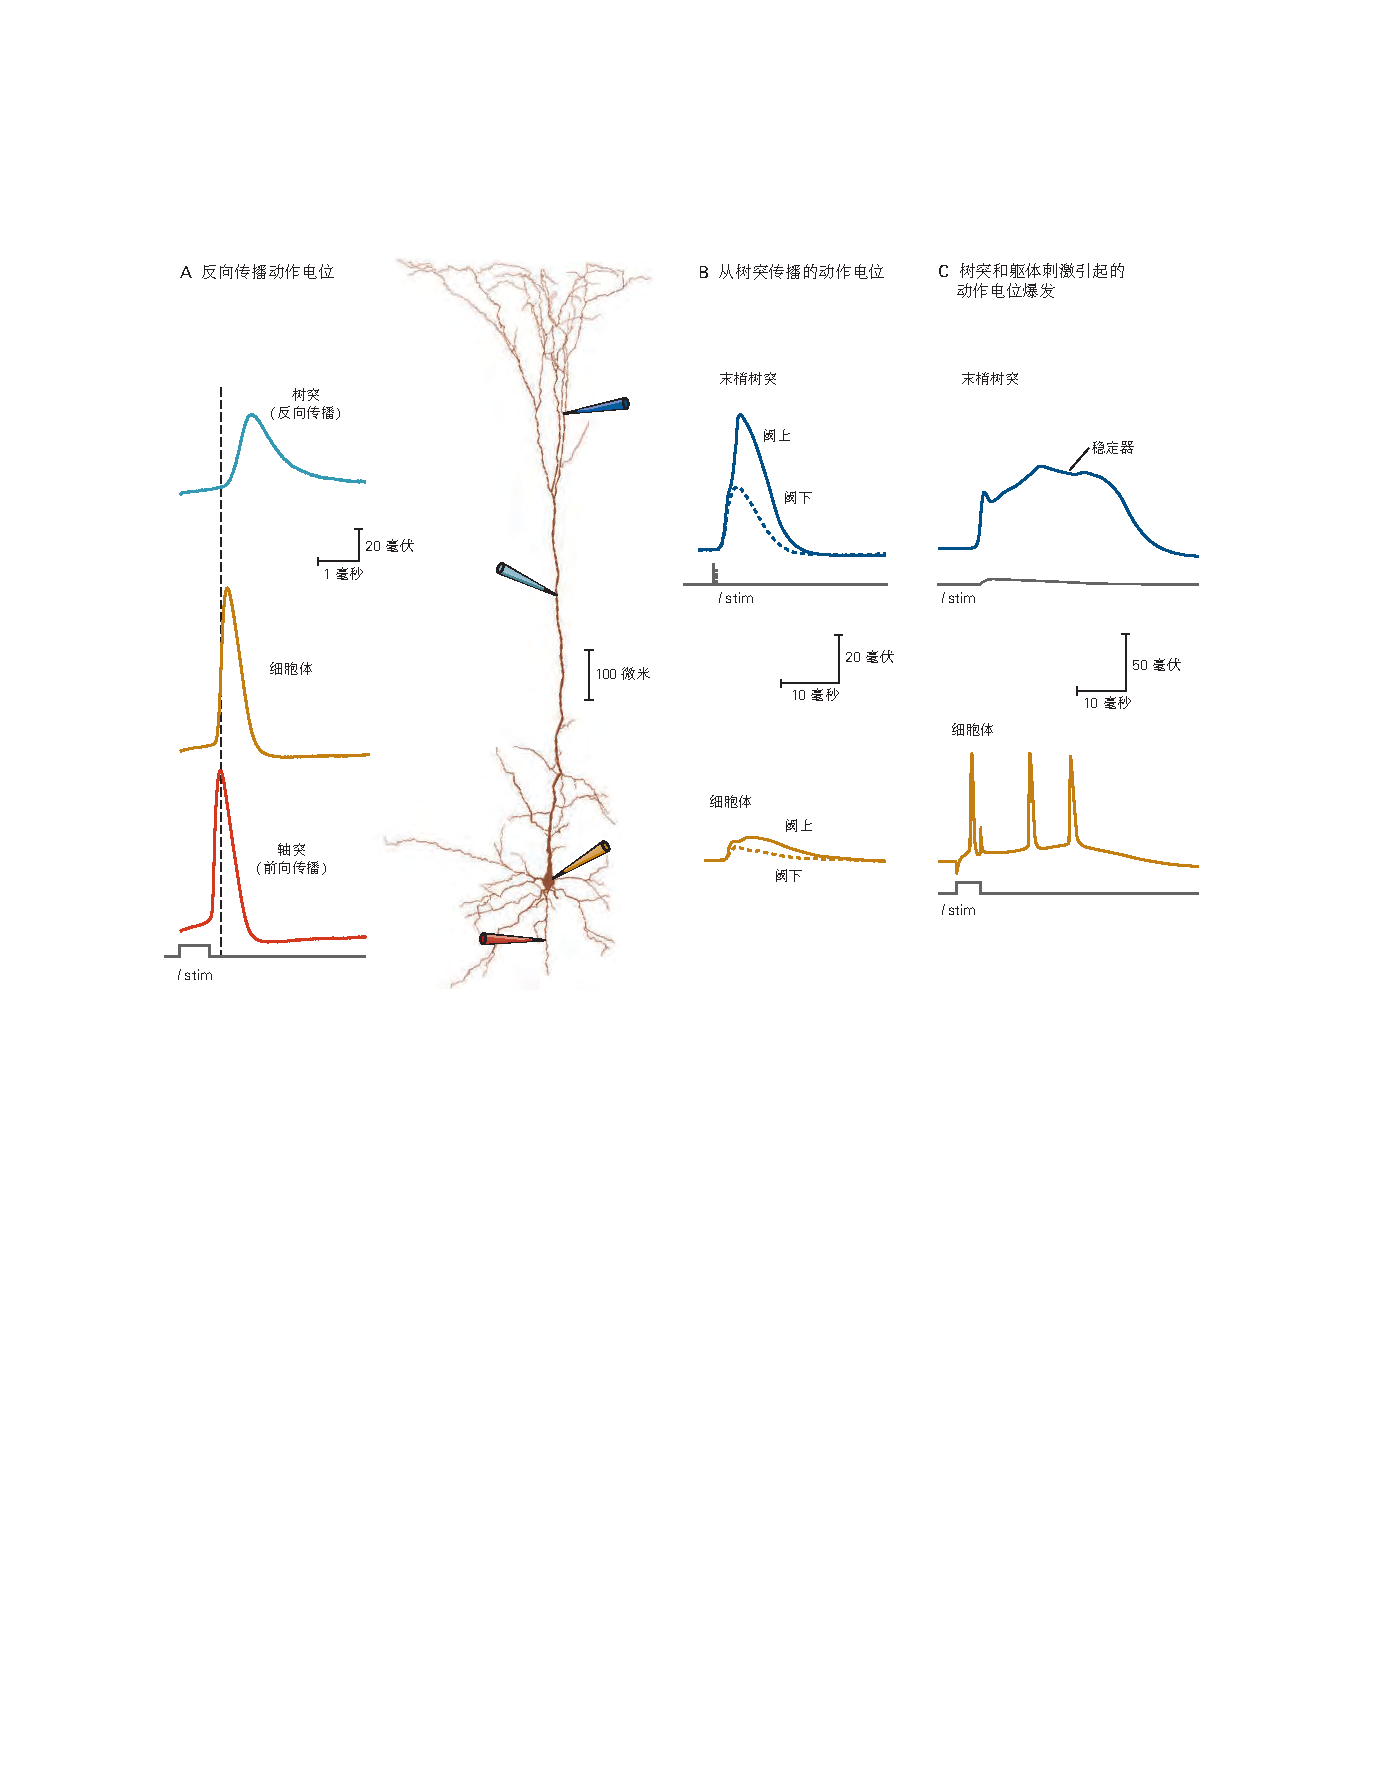
\includegraphics[width=0.95\linewidth]{chap13/fig_13_17}
	\caption{树突的活性特性可以放大突触输入并支持电信号在轴突起始段之间的传播。
		该图说明了一个实验,其中几个电极用于记录膜电压并在轴突、细胞体和树突树的几个位置传递刺激电流。
		记录电极和相应的电压轨迹通过颜色匹配。 还指示了刺激电流脉冲 (I stim)\cite{stuart2016dendrites}。
		\textbf{A.} 在轴突初始段启动的动作电位可以传播到树突。
		这种反向传播取决于树突中电压门控 \ce{Na+} 通道的激活。
		与沿轴突不断再生的非递减动作电位不同,反向传播动作电位的振幅会随着其沿树突传播而降低,这是由于其电压门控 \ce{Na+} 通道密度相对较低。
		\textbf{B.} 树突处的强去极化\textit{兴奋性突触后电位}可以产生传播到细胞体的树突动作电位。
		这种动作电位通常由树突状电压门控 \ce{Ca^2+} 通道产生,并且具有高阈值。
		它们传播相对较慢并且随着距离的增加而衰减,通常无法到达细胞体。
		蓝色实线表示树突响应大去极化电流脉冲而产生的超阈值响应,蓝色虚线表示对较弱电流刺激的亚阈值响应。
		橙色实线和虚线显示了细胞体中记录的相应电压响应。
		\textbf{C.} 将类似弱 EPSC 的亚阈值刺激电流几乎同时注入树突,并在细胞体中注入短暂的强阈上刺激电流(其本身会引起单个体动作电位)触发树突中持久的平台电位和放电 细胞体中的动作电位爆发\cite{larkum1999new}。}
	\label{fig:13_17}
\end{figure}


树突电压门控通道还允许在轴突初始段产生的动作电位向后传播到树突树中(图~\ref{fig:13_17} B)。
这些反向传播动作电位主要由树突状电压门控 \ce{Na+} 通道产生。
虽然这些动作电位的确切作用尚不清楚,但它们可能提供一种时间上精确的机制,通过提供去除 \ce{Mg^2+} 阻滞所需的去极化来增强通过\textit{N-甲基-D-天冬氨酸}受体通道的电流,从而有助于诱导突触可塑性(图~\ref{fig:13_10}) )。


由于其电压依赖性,\textit{N-甲基-D-天冬氨酸}受体能够介导树突中另一种类型的非线性整合。
适度的突触刺激能够激活足够数量的\textit{$\alpha$-氨基-3-羟基-5-甲基异恶唑-4-丙酸}受体以产生中等水平的去极化,从而能够导致 \ce{Mg^2+} 从一部分\textit{N-甲基-D-天冬氨酸}受体中排出。
当这些受体开始将阳离子传导到突触后树突中时,它们会产生进一步的去极化,从而导致更大程度的 \ce{Mg^2+} 解阻,进一步增加\textit{N-甲基-D-天冬氨酸}受体 EPSC 的大小,从而导致更大的去极化。
在某些情况下,这会导致局部再生去极化,称为\textit{N-甲基-D-天冬氨酸}峰值。
这种\textit{N-甲基-D-天冬氨酸}尖峰纯粹是局部事件——它们不能在没有突触刺激的情况下主动传播,因为它们需要释放谷氨酸。
\textit{N-甲基-D-天冬氨酸}峰值与不同形式的突触可塑性和增强突触输入的树突整合有关。


在什么条件下活性电导会影响树突整合?
现在有证据表明,树突可能会根据突触输入的精确时间和强度在被动和主动整合之间切换。
这种转换的一个有趣例子是一些皮层神经元对到达其远端和近端树突的输入作出反应的方式。
在许多神经元中,来自相对较近的神经元的输入到达树突的更近端区域,更靠近细胞体。
来自更远脑区的输入到达树突的远端尖端。
尽管远端树突的兴奋性突触输入通常只在体细胞产生非常小的去极化反应,但由于沿着树突电缆的电子衰减,这些输入与树突更近端区域的兴奋性输入配对时可以显着增强尖峰放电。
因此,近端部位的单个强\textit{兴奋性突触后电位}(或单个短暂的体细胞电流脉冲)通常会在轴突起始段产生单个动作电位,然后可以反向传播到树突中。
然而,当远端刺激与近端刺激配对时,反向传播尖峰与远端\textit{兴奋性突触后电位}相加,触发一种持久类型的树突状尖峰,称为平台电位,这取决于电压门控 \ce{Ca^2+} 通道和\textit{N-甲基-D-天冬氨酸}受体的激活。
当平台电位到达细胞体时,它可以以高达 100 Hz 的速率触发三个或更多尖峰的短暂爆发(图~\ref{fig:13_17} C)。
这些尖峰脉冲被认为提供了一种非常有效的方法来诱导长期突触可塑性并在脉冲传播到突触前末梢时释放递质。


一种更局部化的突触整合形式发生在树突棘中。
尽管一些兴奋性输入发生在树突状轴上,但大脑中接近 95\% 的兴奋性输入终止于棘突,令人惊讶地避免了树突状轴(见图~\ref{fig:13_2})。
虽然棘的功能尚未完全了解,但它们的细颈为各种信号分子从棘头扩散到树突轴提供了屏障。
因此,通过\textit{N-甲基-D-天冬氨酸}受体的相对较小的 \ce{Ca^2+} 电流可导致 [\ce{Ca^2+}] 相对较大的增加,该 [\ce{Ca^2+}] 位于被突触激活的单个脊柱头部(图~\ref{fig:13_18} A)。
此外,由于动作电位可以从细胞体反向传播到树突,因此棘也可以作为整合突触前和突触后活动信息的场所。


\begin{figure}[htbp]
	\centering
	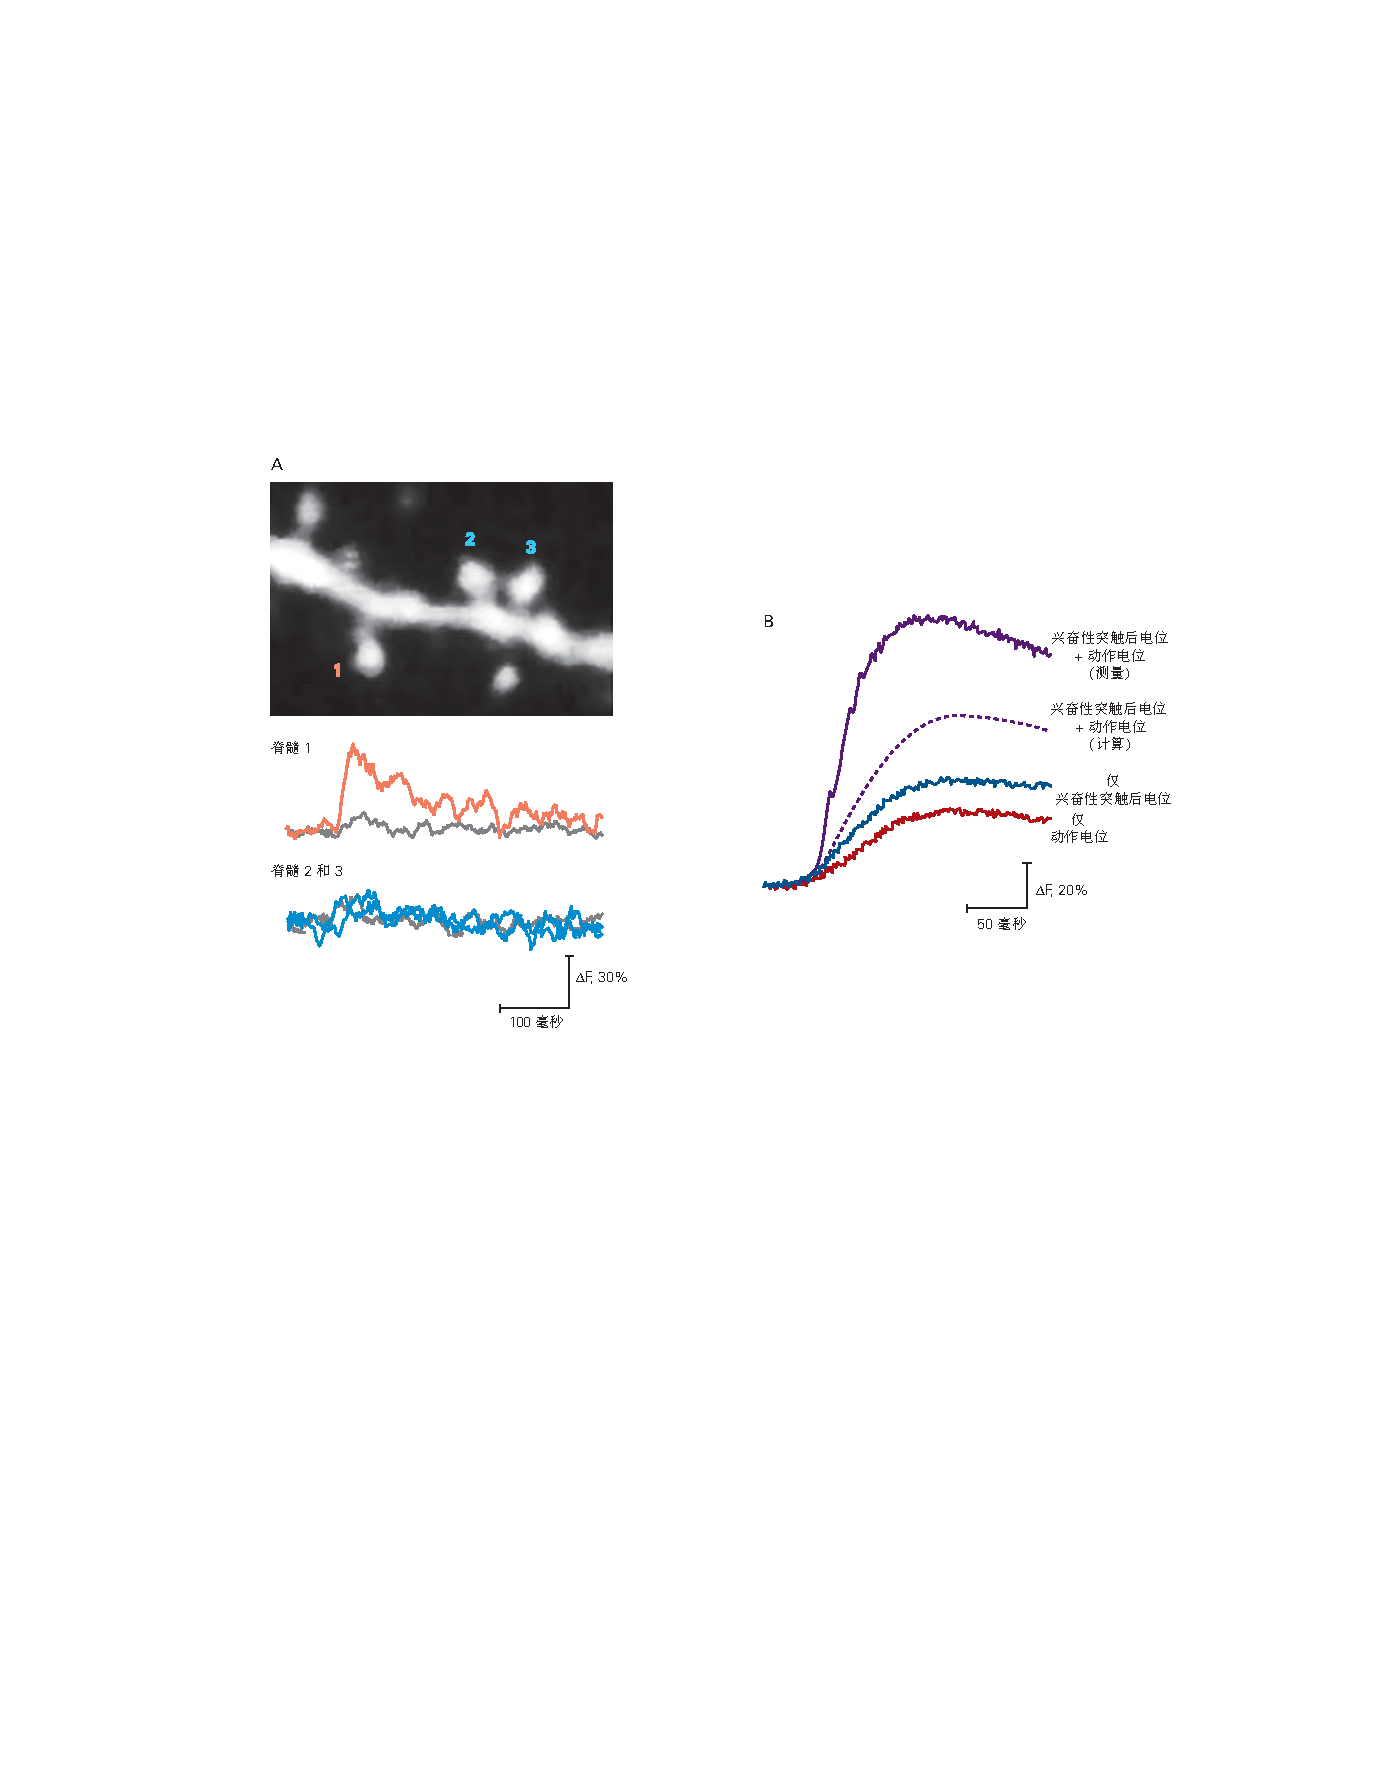
\includegraphics[width=0.4\linewidth]{chap13/fig_13_18}
	\caption{树突棘通过\textit{N-甲基-D-天冬氨酸}受体分隔钙流入。
		\textbf{A.} 这张充满钙敏感染料的海马 CA1 锥体神经元的荧光图像显示了具有多个棘的树突轴的轮廓。
		当染料结合 \ce{Ca^2+} 时,其荧光强度会增加。
		在突触前轴突的细胞外刺激后,这些痕迹绘制了一段时间内的荧光强度。
		脊柱 1 显示响应突触刺激(红色迹线)的荧光 (ΔF) 大量快速增加,反映了通过\textit{N-甲基-D-天冬氨酸}受体的 \ce{Ca^2+} 流入。
		相反,相邻树突轴(灰色迹线)的荧光强度几乎没有变化,表明 \ce{Ca^2+} 积累仅限于脊柱头部。
		脊柱 2 和 3 显示出对突触刺激的荧光几乎没有增加,因为它们的突触前轴突没有被激活\cite{lang2004transient}。 
		\textbf{B.} 当突触刺激与突触后动作电位配对时,脊柱中的钙积累最多。
		同时诱发\textit{兴奋性突触后电位}和反向传播动作电位时生成的 \ce{Ca^2+} 信号大于单独诱发\textit{兴奋性突触后电位}或反向传播动作电位 (AP) 时单个 \ce{Ca^2+} 信号的预期总和\cite{yuste1995dendritic}。}
	\label{fig:13_18}
\end{figure}


事实上,当反向传播动作电位与突触前刺激配对时,脊柱 \ce{Ca^2+} 信号大于来自单独突触刺激或单独动作电位刺激的单个 \ce{Ca^2+} 信号的线性总和。
这种“超线性”特定于激活的脊柱,并且发生是因为动作电位期间的去极化导致 \ce{Mg^2+} 从\textit{N-甲基-D-天冬氨酸}受体通道中排出,使其能够将 \ce{Ca^2+} 传导到脊柱中。
因此,由此产生的 \ce{Ca^2+} 积累在单个突触处提供了输入 (\textit{兴奋性突触后电位}) 和输出(反向传播动作电位)的近乎同时性的生化检测器,这被认为是记忆存储的关键要求(第~\ref{chap:chap34}~章)。


因为细的脊柱颈至少部分地限制了 \ce{Ca^2+} 的升高,从而限制了接收突触输入的脊柱的长期可塑性,因此脊柱还确保突触功能的活动依赖性变化,以及记忆存储,是仅限于被激活的突触。
脊柱实现这种特定于突触的局部学习规则的能力对于神经网络存储有意义信息的能力可能具有根本的重要性(第 ~\ref{chap:chap54}~章)。
最后,在一些棘中,局部突触电位在通过棘颈传播并进入树突时被过滤,从而减小细胞体处\textit{兴奋性突触后电位}的大小。
这种电过滤的调节可以提供另一种控制给定突触电导能够激发细胞体的功效的方法。



\section{亮点}

1. 一个典型的中枢神经元整合了大量的兴奋性和抑制性突触输入。
氨基酸递质谷氨酸负责中枢神经系统中大多数兴奋性突触作用,抑制性氨基酸\textit{$\gamma$-氨基丁酸}和甘氨酸介导抑制性突触作用。 


2. 谷氨酸激活离子型和代谢型受体家族。
三种主要的离子型谷氨酸受体——\textit{$\alpha$-氨基-3-羟基-5-甲基异恶唑-4-丙酸}、\textit{N-甲基-D-天冬氨酸}和红藻氨酸——以激活它们的化学激动剂命名。 


3.离子型谷氨酸受体是由同源基因编码的亚基组成的四聚体。
每个亚基都有一个大的细胞外氨基末端,具有三个跨膜片段和一个大的细胞质尾部。
成孔环在第一和第二跨膜区段之间浸入和浸出膜。 


4. 谷氨酸与所有三种离子型受体的结合打开了一个对 \ce{Na+} 和 \ce{K+} 具有同等渗透性的非选择性阳离子通道。
\textit{N-甲基-D-天冬氨酸}受体通道对 \ce{Ca^2+} 也具有高渗透性。


5. \textit{N-甲基-D-天冬氨酸}受体充当符合检测器。
它通常被滞留在其孔隙中的细胞外 \ce{Mg^2+} 阻断;
它仅在释放谷氨酸并且突触后膜充分去极化以通过静电排斥排出\ce{Mg^2+}离子时才进行。 


6. 在强烈的突触激活过程中,通过\textit{N-甲基-D-天冬氨酸}受体的钙流入可以触发细胞内信号级联,导致长期突触可塑性,这可以加强突触传递数小时至数天,为记忆存储提供潜在机制。 


7. 大脑中的抑制性突触作用是由\textit{$\gamma$-氨基丁酸}与离子型 (\textit{$\gamma$氨基丁酸A}) 和代谢型 (GABAB) 受体的结合介导的。
\textit{$\gamma$氨基丁酸A} 受体是五聚体,其亚基与烟碱\textit{乙酰胆碱}受体的亚基同源。
甘氨酸离子型受体在结构上类似于 \textit{$\gamma$氨基丁酸A} 受体,主要局限于脊髓中的抑制性突触。 


8. \textit{$\gamma$-氨基丁酸}或甘氨酸与其受体的结合会激活 \ce{Cl-} 选择性通道。
在大多数细胞中,\ce{Cl-} 平衡电位略低于静息电位。
结果,抑制性突触作用使细胞膜超极化,远离触发动作电位的阈值。 


9. 神经元是否激发动作电位的决定取决于各种兴奋性和抑制性输入的空间和时间总和,并由轴突起始段所产生的去极化的大小决定,神经元具有最低的区域临界点。 


10. 树突也有电压门控通道,使它们能够在某些情况下激发局部动作电位。
这可以放大局部\textit{兴奋性突触后电位}的大小,从而在细胞体处产生更大的去极化。






